\documentclass[
ngerman, % neue Deutsche Rechtschreibung
headings=normal, % normale Headings
captions=tableheading, % places caption above tables
listof=totoc,
bibliography=totoc,
final
%usegeometry, % Auskommentieren wenn Package geometery verwendet wird
%DEBUGGING
%draft, % entfernen nach abschluss der bearbeitung
%overfullrule, % entfernen nach abschluss der bearbeitung
% Default Values
%oneside, % Einseitige Seitengenerierung
%11pt, % Font size
% a4paper, % paper
]{scrreprt}
\KOMAoptions{%
  DIV=12,
  parskip=half*,
% %BCOR=korrektur, % absoluter Wert der Bindekorrektur
}

% Meta-Daten zu dieser Arbeit ------------------------------------------------------------
\newcommand{\titel}{Evaluation der Reinforcement Learning Algorithmen Sarsa und \mbox{Q-Learning} am Beispiel eines Strategiespiels\xspace}
\newcommand{\art}{Bachelorarbeit\xspace}
\newcommand{\studiengang}{Wirtschaftsinformatik B.Sc. dual}

\newcommand{\autor}{Jonas Bingel}
\newcommand{\strasseAutor}{\censor{Musterstr. 00}}
\newcommand{\stadtAutor}{\censor{65000} Wiesbaden}
\newcommand{\matrikelnr}{\censor{123456}}

\newcommand{\unternehmen}{Unternehmen}
\newcommand{\datumAblaufSperrvermerk}{01.01.1970}

\newcommand{\betreuer}{Prof. Dr. Frank Mehler}
\newcommand{\datumAbgabe}{28.02.2022}
\newcommand{\ort}{Wiesbaden}
\newcommand{\logo}{logo_hsmz.png}

\usepackage[utf8]{inputenc}
\usepackage[T1]{fontenc}
\usepackage{babel}
\usepackage{lmodern}
\usepackage{xspace} % Leerzeichen hinter parameterlosen Makros nicht als Endzeichen interpretieren
\usepackage{graphicx}
\usepackage{pdfpages}
\includepdfset{scale=0.7, frame, pagecommand={\thispagestyle{plain}}}
\graphicspath{{04_Artefakte/01_Abbildungen/}}
\usepackage{caption}
\usepackage{subcaption} % https://www.ctan.org/pkg/subcaption

\usepackage{tabularx}
\usepackage{booktabs}
\usepackage[longtable]{multirow}
\usepackage{longtable}

\usepackage{amsmath}
\usepackage{amsfonts}
\usepackage{bbm}

\usepackage{xcolor}
%\usepackage{chngcntr} % fortlaufende Nummerierung von Fußnoten

\usepackage[colorinlistoftodos, disable]{todonotes} % to disable todos use option disable, alternatively use obeyDraft or obeyFinal
\usepackage{blindtext}

\usepackage{microtype} % auskommentieren moeglich, wenn Typografie nicht zufriedenstellend

\usepackage[bottom]{footmisc} % https://golatex.de/viewtopic.php?f=21&t=24052
% Verlinkung und PDF Bookmarks https://tex.stackexchange.com/a/83051
\usepackage[nospace]{varioref}
% extensions keep all links black, only urls are blue: https://tex.stackexchange.com/a/401885/220502
\usepackage[hidelinks, colorlinks, allcolors=., urlcolor=blue]{hyperref}
\usepackage{bookmark}
\hypersetup{
    pdftitle={\titel},
    pdfauthor={\autor},
    pdfcreator={\autor},
    pdfsubject={\titel},
    pdfkeywords={\titel},
}
\usepackage{cleveref}

% Literaturverzeichnis und Quellenverwaltung mittels biblatex
\usepackage[%
backend=biber,
style=ieee,
dashed=false,
% APA style
%sortlocale=auto,
%sorting=nyt,
%style=apa
]{biblatex}


% Verwalten von Abkuerzungen und einem Abkuerzungsverzeichnis
\usepackage[printonlyused]{acronym} % https://www.ctan.org/pkg/acronym


% Packages for forcing floats https://robjhyndman.com/hyndsight/latex-floats/
\usepackage{afterpage}
\usepackage[section]{placeins}
\usepackage{censor}


% Erstellen eines Symbolverzeichnisses
\usepackage[intoc, german, stdsubgroups]{nomencl} % https://www.ctan.org/pkg/nomencl
\usepackage{siunitx}
\newcommand{\nomunit}[1]{%
    \renewcommand{\nomentryend}{\hspace*{\fill}\si{#1}}}
\makenomenclature

\usepackage[newfloat, cache]{minted} % https://www.ctan.org/pkg/minted
\SetupFloatingEnvironment{listing}{name=Listing, placement=b}
\SetupFloatingEnvironment{listing}{listname={Listingverzeichnis}}
\setminted[java]{linenos, fontsize=\footnotesize, frame=lines, breaklines, breakbefore={.}}
\usemintedstyle{borland}
% new environment for listings longer than one page; https://tex.stackexchange.com/a/53540
\newenvironment{longlisting}{\captionsetup{type=listing}}{}
\usepackage{csquotes}


% Darstellung von Algorithmen und Pseudocode
% do NOT use option naturalnames if you compile with pdflatex and use hyperref
\usepackage[linesnumbered, commentsnumbered, ruled]{algorithm2e} 
\renewcommand{\listalgorithmcfname}{Algorithmusverzeichnis}
\addtotoclist[float]{loa}
\renewcommand\listofalgorithms{\listoftoc[{\listalgorithmcfname}]{loa}}
%\SetAlFnt{\small \normalfont \sffamily} 
\SetAlFnt{\footnotesize} 


% Erstellung neuer Verzeichnisse; Code weitgehend von Markus Kohm und komascript.de 
\DeclareNewTOC[%
  owner=anhang,
  listname={Anhangsverzeichnis},% Titel des Verzeichnisses
]{atoc}

\DeclareNewTOC[%
  type=equation,
  listname={Formelverzeichnis},
  tocentrynumwidth=2.3em,
]{loe}

\makeatletter
\renewcommand\@pnumwidth{2em} % vermeiden von overful hbox im Inhaltsverzeichnis

\AfterTOCHead[atoc]{\let\if@dynlist\if@tocleft}
\newcommand*{\useappendixtocs}{%
  \renewcommand*{\ext@toc}{atoc}%
  \scr@ifundefinedorrelax{hypersetup}{}{% damit es auch ohne hyperref funktioniert
    \hypersetup{bookmarkstype=atoc}%
  }%
}
\newcommand*{\usestandardtocs}{%
  \renewcommand*{\ext@toc}{toc}%
  \scr@ifundefinedorrelax{hypersetup}{}{% damit es auch ohne hyperref funktioniert
    \hypersetup{bookmarkstype=toc}%
  }%
  \renewcommand*{\ext@figure}{lof}%
  \renewcommand*{\ext@table}{lot}%
}
\scr@ifundefinedorrelax{ext@toc}{%
  \newcommand*{\ext@toc}{toc}
  \renewcommand{\addtocentrydefault}[3]{%
    \expandafter\tocbasic@addxcontentsline\expandafter{\ext@toc}{#1}{#2}{#3}%
  }
}{}
\newcommand*{\@currententry}{}
% Zwei amsmath-Anweisungen ändern:
\g@addto@macro\make@display@tag{\set@currententry}%
\def\tagform@#1{\maketag@@@{(\ignorespaces#1\unskip\@@italiccorr)}%
  \set@currententry}
\newcommand*{\set@currententry}{%
  \typeout{set current entry}%
  \ifx\@currententry\@empty\else
    \addcontentsline{loe}{equation}{\protect\numberline{\@currentlabel}%
      \@currententry}%
    \global\let\@currententry\@empty
  \fi
}
% Neue Benutzeranweisung
\newcommand*{\equationentry}[1]{%
  \gdef\@currententry{#1}%
}

\makeatother

\usepackage{xpatch}
\xapptocmd\appendix{%
  \useappendixtocs
  \pdfbookmark{Anhangsverzeichnis}{anhangsverzeichnis}
  \listofatocs
  \addcontentsline{toc}{chapter}{Anhangsverzeichnis}
  \bookmarksetupnext{level=-1}
}{}{}

% Pakete, die fuer Informatik Sinn ergeben koennten
% \usepackage{bytefield} % illustration of fields of data https://www.ctan.org/pkg/bytefield


% Uebersetzung fuer Eintraege im Abkuerzungsverzeichnis - Code uebernommen von https://tex.stackexchange.com/a/135507
\makeatletter
\newcommand{\acroforeign}[1]{}

% patch the environment to print the foreign definition:
\AtBeginEnvironment{acronym}{%
  \def\acroforeign#1{ (#1)}%
}

% patch the acronym definition to safe the foreign definition:
\expandafter\patchcmd\csname AC@\AC@prefix{}@acro\endcsname
  {\begingroup}
  {\begingroup\def\acroforeign##1{\csdef{ac@#1@foreign}{##1, }}}
  {}
  {\fail}

% %   renew the first output to include the foreign definition if given:
\renewcommand*{\@acf}[2][\AC@linebreakpenalty]{%
  \ifAC@footnote
    \acsfont{\csname ac@#2@foreign\endcsname\AC@acs{#2}}%
    \footnote{\AC@placelabel{#2}\AC@acl{#2}{}}%
  \else
    \acffont{%
      \AC@placelabel{#2}\AC@acl{#2}%
      \nolinebreak[#1] %
      \acfsfont{(\acsfont{\csname ac@#2@foreign\endcsname\AC@acs{#2}})}%
    }%
  \fi
  \ifAC@starred\else\AC@logged{#2}\fi
}
\makeatother

% Adjusting the width that is reserved for the  pagenumber in listings
% https://projekte.dante.de/DanteFAQ/Verzeichnisse#2
% https://de.comp.text.tex.narkive.com/fAP3Znev/overfull-hbox-im-inhaltsverzeichnis
\makeatletter
\AtBeginDocument{
\newlength{\mylen}
\setlength{\mylen}{\widthof{XXIII}}
\renewcommand*\@pnumwidth{\the\mylen}
}
\makeatother
% Generelle QoL Anweisungen ------------------------------------------------------------

% Befehle zu Abkuerzungen --------------------------------------------------------------
% Die Anweisung \, erzeugt einen kurzen Abstand und wird bei Abkuerzungen oder zwischen Zahlen und Masseinheiten verwendet
\newcommand{\bs}{$\backslash$\xspace}
\newcommand{\ua}{\mbox{u.\,a.}\xspace}
\newcommand{\oa}{\mbox{o.\,a.}\xspace}
\newcommand{\bspw}{bspw.\xspace}
\newcommand{\bzw}{bzw.\xspace}
\newcommand{\ca}{ca.\xspace}
\newcommand{\dahe}{\mbox{d.\,h.}\xspace}
\newcommand{\etc}{etc.\xspace}
\newcommand{\eur}[1]{\mbox{#1\,\texteuro}\xspace}
\newcommand{\evtl}{evtl.\xspace}
\newcommand{\ggfs}{ggfs.\xspace}
\newcommand{\Ggfs}{Ggfs.\xspace}
\newcommand{\gqq}[1]{\glqq{}#1\grqq{}}
\newcommand{\idR}{i.d.R.\xspace}
\newcommand{\inkl}{inkl.\xspace}
\newcommand{\exkl}{exkl.\xspace}
\newcommand{\insb}{insb.\xspace}
\newcommand{\usw}{usw.\xspace}
\newcommand{\Vgl}{Vgl.\xspace}
\newcommand{\sogn}{sogn.\xspace}
\newcommand{\zB}{\mbox{z.\,B.}\xspace}
\newcommand{\engl}{engl.\xspace}
\newcommand{\dt}{dt.\xspace}

\newcommand{\splay}{Self-play\xspace}
\newcommand{\qlearning}{Q-Learning\xspace}
\newcommand{\bothAlgs}{Q-Learning und Sarsa\xspace}
\newcommand{\sarsa}{Sarsa\xspace}
\newcommand{\expertplay}{Expert Play\xspace}
\newcommand{\qtable}{Q-Tabelle\xspace}
\newcommand{\wtable}{W-Tabelle\xspace}
\newcommand{\qValue}{Q-Value\xspace}
\newcommand{\qValues}{Q-Values\xspace}
\newcommand{\wValue}{W-Value\xspace}
\newcommand{\wValues}{W-Values\xspace}
\newcommand{\satuple}{SA Tupel\xspace}
\newcommand{\ttt}{Tic-Tac-Toe\xspace}
\newcommand{\statevalueFunktion}{State-Value Funktion\xspace}
\newcommand{\actionValueFunktion}{Action-Value Funktion\xspace}
\newcommand{\afterStateVFunction}{Afterstate-Value Funktion\xspace}
\newcommand{\qFunction}{Q-Funktion\xspace}
\newcommand{\afterstateTable}{Afterstate-Tabelle\xspace}




% Custom Anweisungen ------------------------------------------------------------------
\newcommand\includepdfWithChapter[4]{%
\includepdf[pages={#1}, pagecommand={\chapter{#3}}]{#4}
\includepdf[pages={#2}]{#4}
}




% Typesetting options

\widowpenalty=10000     % Hurenkinder
\clubpenalty=10000      % Schusterjungen

\addbibresource{zotero.bib}
%\nocite{*} % TODO entfernen nur zum draften
\newcounter{romanConsecutive}

\begin{document}
\listoftodos





\pagestyle{empty}
\renewcommand*{\chapterpagestyle}{empty}
%\pdfbookmark{Sperrvermerk}{sperrvermerk}
\addchap*{Sperrvermerk}
Die vorliegende \art mit dem Titel \titel enth"alt interne und vertrauliche Daten des Unternehmens/der Einrichtung \unternehmen.

Die \art darf nur den Gutachtern (insbesondere Erst- und Zweitgutachtern), den Mitgliedern der Prüfungsorgane (einschließlich Beisitzer \& Plagiatskontrolle) sowie den in einem eventuellen Rechtschutzverfahren Betrauten zug"anglich gemacht werden.

Im "Ubrigen ist eine Ver"offentlichtung und Vervielf"altigung der Abschlussarbeit -- auch in Auszügen -- nicht gestattet. Vorbehaltlich der Vorschriften zum Pr"ufungsverfahren und der Pr"ufung bedarf eine Einsichtnahme in die Arbeit durch Dritte einer ausdr"ucklichen Genehmigung der Verfasserin/des Verfassers sowie des \oa Unternehmens.

Diese Geheimhaltungsverpflichtung gilt bis zum Ablauf des \datumAblaufSperrvermerk.

\begin{titlepage}

\begin{minipage}{\textwidth}
		\noindent \hfill \includegraphics{\logo}
\end{minipage}
\vspace{6em}

\begin{center}
    {\huge \art}
    
    {\Large Studiengang \studiengang}
    
    \vspace{4em}
    
    \textbf{{\Large \titel}}
    
    \vspace{4em}
    
    Hochschule Mainz
    
    University of Applied Sciences

    Fachbereich Wirtschaft
    
    \vspace{6em}

	\begin{minipage}{\textwidth}
		\begin{tabbing}
		
		Vorgelegt von:  \hspace*{2em}\= \autor \\
		\> \strasseAutor \\
        \> \stadtAutor \\
        \> Matrikel-Nr. \matrikelnr \\
        Vorgelegt bei: \> \betreuer \\
        Eingereicht am: \> \datumAbgabe
		\end{tabbing}

	\end{minipage}
\end{center}
\end{titlepage}

\pdfbookmark{Erkl"arung}{erklaerung}
\addchap*{Erkl"arung}
Hiermit erkl"are ich, dass ich die vorliegende \art
\begin{quote}
\textbf{\titel}   
\end{quote}

selbstst"andig und ohne fremde Hilfe angefertigt habe. 
Ich habe dabei nur die in der Arbeit angegebenen Quellen und Hilfsmittel benutzt.

Zudem versichere ich, dass ich weder diese noch inhaltlich verwandte Arbeiten als Pr"ufungsleistung in anderen F"achern eingereicht habe oder einreichen werde.

\vspace{1.5cm}
% \begin{figure}[h]
%     \hspace{9cm}
%     \includegraphics[scale=0.2]{04_Artefakte/01_Abbildungen/signature.png}
% \end{figure}
\ort, den \datumAbgabe \hfill \autor 



\pdfbookmark{Management Summary}{summary}
\addchap*{Management Summary}
Die vorliegende Bachelorarbeit befasst sich mit Reinforcement Learning, das ein Teilgebiet des Machine Learning ist. 
Reinforcement Learning und die zugehörigen Methoden zur Lösung sequenzieller Entscheidungsprobleme werden erklärt und von den anderen Teilgebieten des Machine Learning abgegrenzt.
Der Fokus der Arbeit liegt auf dem Teilgebiet des Temporal-Difference Learning und den Algorithmen Q-Learning und Sarsa.
Die Arbeit erläutert das Konzept von Temporal-Difference Learning. Basierend darauf werden Q-Learning und Sarsa erklärt und miteinander verglichen.
Zur weiteren Evaluation der Algorithmen werden diese für das Strategiespiel Tic-Tac-Toe in Java implementiert.
Es wird untersucht, ob beide Algorithmen das Spiel durch Spiele gegen sich selbst erlernen können und welche Auswirkungen verschiedene Hyperparameter auf das Training haben.
Die trainierten Agenten werden auf Basis der Rate optimaler Aktionen während des Trainings und der erreichten Spielstärke verglichen.
Die Auswertung zeigt, dass Q-Learning im Durchschnitt schneller konvergiert und eine höhere Spielstärke erreicht als Sarsa.


\pagestyle{plain}
\renewcommand*{\chapterpagestyle}{plain}
\pagenumbering{Roman}
% Inhaltsverzeichnis ----------------------------------------------------------------------
\pdfbookmark{Inhaltsverzeichnis}{inhaltsverzeichnis}
\tableofcontents

% Abbildungsverzeichnis -------------------------------------------------------------------
\listoffigures

% Tabellenverzeichnis ---------------------------------------------------------------------
\listoftables

% Abkuerzungsverzeichnis ------------------------------------------------------------------

\newcommand{\abksvz}{Abk"urzungsverzeichnis}
\chapter*{\abksvz}
\addchaptertocentry{}{\abksvz}
\begin{acronym}
	\acro{MDP}{Markov Decision Process \acroforeign{\dt Markov-Entscheidungsprozess}}
	\acro{ML}{Machine Learning \acroforeign{\dt Maschinelles Lernen}}
	\acro{RL}{Reinforcement Learning \acroforeign{\dt. bestärkendes Lernen}}
	\acro{SA Tupel}{State-Action Tupel \acroforeign{\dt Zustand-Aktion Tupel}}
	\acro{TD}{Temporal-Difference}
	\acro{TDL}{Temporal-Difference Learning}
	\acro{TTT}{\ttt}
\end{acronym}

% Symbolverzeichnis -----------------------------------------------------------------------
\printnomenclature

% Formelverzeichnis -----------------------------------------------------------------------
\listofequations

% Listingverzeichnis ----------------------------------------------------------------------
\listoflistings

% Algorithmenverzeichnis ------------------------------------------------------------------
\listofalgorithms

\nomenclature[aa]{$\mathbbm{E}$}{Erwartungswert}
\nomenclature[ab]{$\mathbbm{1}_{prädikat}$}{Indikatorfunktion, 1 wenn das Prädikat wahr ist, sonst 0}

\nomenclature[ac]{$s,s'$}{Zustände in einem \acs{MDP}, $s'$ ist der Folgezustand}
\nomenclature[ad]{$A(s)$}{Menge aller möglichen Aktionen in einem Zustand $s$}
\nomenclature[ae]{$a$}{eine Aktion in einem \acs{MDP}}
\nomenclature[af]{$r$}{ein Reward in einem \acs{MDP}}

\nomenclature[ag]{$t$}{diskreter Zeitschritt}
\nomenclature[ah]{$T$}{letzter Zeitschritt einer Episode}

\nomenclature[ai]{$S$}{Menge aller Zustände ohne Terminalzustände}
\nomenclature[aj]{$S^+$}{Menge aller Zustände \inkl Terminalzustände}
\nomenclature[ak]Y{Menge aller Afterstates}
\nomenclature[al]y{ein Afterstate}
\nomenclature[am]w{\wValue eines Afterstates}
\nomenclature[an]{$S_t$}{Zustand der Umgebung zum Zeitschritt $t$}
\nomenclature[as]{$S_T$}{Terminalzustand}
\nomenclature[at]{$A_t$}{Aktion, die Agent im  Zeitschritt $t$ wählt}
\nomenclature[au]{$R_t$}{Reward, der im  Zeitschritt $t$ ausgegeben wird}
\nomenclature[av]{$G_t$}{Return, kumulierter Reward nach Zeitschritt $t$}

\nomenclature[aw]{$v_\pi$}{State-Value Funktion zur Policy $\pi$}
\nomenclature[ax]{$v_*$}{optimale State-Value Funktion}
\nomenclature[ay]{$V$}{Schätzwert für die State-Value Funktion}

\nomenclature[az]{$q_\pi$}{Action-Value Funktion zur Policy $\pi$}
\nomenclature[az1]{$q_*$}{optimale Action-Value Funktion}
\nomenclature[az2]{$Q$}{Schätzwert für die Action-Value Funktion}


\nomenclature[az3]{$B_G$}{Bitboard einer Spielfeldkonstellation, das Symbole nicht unterscheidet}
\nomenclature[az4]{$B_X$}{Bitboard des Symbols X}
\nomenclature[az5]{$B_O$}{Bitboard des Symbols O}
\nomenclature[az6]{$B_s$}{Bitboard des Zustands $s$}


\nomenclature[gp]{$\pi$}{eine Policy}
\nomenclature[gp1]{$\pi_*$}{optimale Policy}
\nomenclature[ga]{$\alpha$}{Lernrate}
\nomenclature[gc]{$\gamma$}{Diskontierungsfaktor}
\nomenclature[gd]{$\delta_t$}{Temporal-Difference Error zum Zeitschritt $t$}
\nomenclature[ge]{$\epsilon$}{Explorationswahrscheinlichkeit}




\setcounter{romanConsecutive}{\value{page}}
\pagenumbering{arabic}
\chapter{Einleitung}
\section{Motivation}
Ein zentrales Teilgebiet Künstlicher Intelligenz ist \ac{ML}, das sich mit Methoden befasst, um Computer aus Erfahrungen, in Form von Trainingsdaten, lernen zu lassen \cite[S. 178]{ertelIntroductionArtificialIntelligence2017}, \cite[S. 524]{russellArtificialIntelligenceModern2021}. 
Jedoch ist es bei interaktiven Anwendungen nicht praktikabel repr"asentative Trainingsdaten für alle Situationen zu erhalten oder die korrekte Entscheidung ist nicht bekannt \cite[S. 24]{suttonReinforcementLearningIntroduction2018}.  
Zudem sind Entscheidungen oft sequenziell und gegebenenfalls muss die Entscheidung getroffen werden auf eine direkte Belohnung zu verzichten, um später eine größere Belohnung zu erhalten \cite[S. 1]{vanderreeReinforcementLearningGame2013}. 

\ac{RL} ist das Teilgebiet von \ac{ML} das sich mit der Erstellung von Agenten beschäftigt, die sequenziell Entscheidungen treffen, um einen Gesamtgewinn zu maximieren \cite[S. 1]{vanderreeReinforcementLearningGame2013}, \cite[S. 1]{suttonReinforcementLearningIntroduction2018}.  
Dafür interagiert ein Agent mit seiner Umgebung (\engl Environment), um Erfahrungen zu sammeln und aus diesen, ohne zusätzlich eingebrachtes Wissen zu lernen. 
Aufgrund dieser Eigenschaft ist \ac{RL} das Teilgebiet von \ac{ML}, das dem menschlichen Lernen am nächsten ist. \cite[S. 4]{suttonReinforcementLearningIntroduction2018}

Zu einer Anwendung und Evaluation von \ac{RL} Algorithmen eigenen sich (Strategie-)spiele, insbesondere wegen des sequenziellen Aufbaus, klar definierten Umgebung und der Reproduzierbarkeit \cite[S. 1]{vanderreeReinforcementLearningGame2013}.
Beispielsweise wurden in \cite{tesauroTemporalDifferenceLearning1992a} und \cite{vanderreeReinforcementLearningGame2013} für die Spiele Backgammon und Othello \ac{RL} Agenten trainiert, die allein durch \splay eine hohe Spielstärke erreichen. 
Beim \splay spielt ein Agent zum Training nur gegen sich selbst und erhält kein externes Wissen. 
Externes Wissen könnte beispielsweise bereitgestellt werden in Form von Expert Play, d.h. Gegnern, die optimalen Spielstrategien folgen und so auf Experten-Niveau spielen \cite[S. 561]{szitaReinforcementLearningGames2012}. 
In beiden Beispielen wurden Algorithmen aus dem \ac{RL} Teilbereich des \ac{TDL} verwendet. 
Zwei richtungsweisende und verbreitete \ac{TDL} Algorithmen sind \qlearning und \sarsa, die eng miteinander verwandt sind \cite[S. 138]{suttonReinforcementLearningIntroduction2018}, \cite[S. 1]{vanderreeReinforcementLearningGame2013}, \cite[S. 1]{samsudenReviewPaperImplementing2019}.

In der vorliegenden Arbeit soll das simple Strategiespiel \ac{TTT} zur Evaluation dieser Algorithmen genutzt werden, das sich aufgrund verschiedener Aspekte dafür eignet. 
Erstens ist \ac{TTT} ein simples und bekanntes Spiel und dadurch ein anschauliches Beispiel \cite[S. 6]{allisSearchingSolutionsGames1994}. 
Zweitens ist \ac{TTT} ein gelöstes Spiel mit optimalen Strategien, was eine Evaluation der Agenten ermöglicht \cite[S. 533ff.]{crowleyFlexibleStrategyUse1993}.
Drittens, besitzt \ac{TTT} einen diskreten und kleinen Zustands- sowie Aktionsraum, sodass Agenten schnell trainiert werden können \cite[S. 3]{block-berlitzm.ProInformatikFunktionaleProgrammierung2009}. 
Außerdem können dieselben Spielzustände durch mehrere Spielabfolgen erreicht werden. 
Dies ermöglicht eine Evaluation des Konzepts der Afterstates (dt. Folgezustände), das die gesammelte Erfahrung effektiver nutzen soll. \cite[S. 136f.]{suttonReinforcementLearningIntroduction2018}

\section{Ziele und Forschungsfragen}
\label{sec:forschungsfragen}
Die vorliegende Arbeit verfolgt zwei zentrale Ziele. Zum einen die Erklärung der \ac{RL} Algorithmen \qlearning und \sarsa sowie die Erarbeitung von deren Unterschieden.
Zum anderen die Anwendung und Evaluation der beiden Algorithmen am Beispiel des  Strategiespiels \ttt. 
Die zentrale Forschungsfrage für das zweite Ziel ist, ob die beiden Algorithmen durch \splay eine hohe Spielstärke erreichen und optimale Spielstrategien bzw. Expert Play erlernen.
Unter diese Forschungsfrage gliedern sich die folgenden weiteren Forschungsfragen:
\begin{itemize}
    \item Eine Abschätzung für die Anzahl der Trainingsepisoden, die  ungefähr benötigt werden, um Expert Play in \ac{TTT} durch Self-play zu erlernen?
    \item Welche Auswirkung hat die Verwendung des Konzepts der Afterstates auf das Konvergenzverhalten und Spielstärke der Agenten?
    \item Was sind die besten Hyperparameter für \bothAlgs?
    \item Wie unterscheiden sich \bothAlgs hinsichtlich ihrer Konvergenz?
    \item Welcher Agent erreicht eine bessere Spielstärke, wenn beide Algorithmen mit ihren optimalen Hyperparametern trainiert werden?
    \item Was ist aus Sicht der Agenten die optimale erste Aktion?
\end{itemize}

\section{Aufbau der Arbeit}
Die vorliegende Bachelorarbeit gliedert sich inklusive dieser Einleitung in sechs Kapitel. 
Kapitel 2 dient der Darstellung der Grundlagen, die notwendig sind, um die Algorithmen \bothAlgs zu verstehen und auf \ac{TTT} anwenden und evaluieren zu können. 
Dazu werden die Bestandteile von \ac{RL} und das zu implementierende Spiel erklärt und die beiden Algorithmen verglichen. 
Kapitel 3 beschreibt die Methodik und Anwendung der Algorithmen auf \ac{TTT} sowie die Kodierung des Spiels selbst. 
Anschließend wird der gewählte Trainingsaufbau der Agenten und die Evaluation mit den zugehörigen Metriken vorgestellt. 
In Kapitel 4 wird die gewählte Architektur sowie die Implementierung in Java vorgestellt. 
Kapitel 5 diskutiert die Ergebnisse der Evaluation der Algorithmen und vergleicht diese. 
Anschließend werden auf Basis der gesammelten Erkenntnisse die Forschungsfragen beantwortet. 
Zum Schluss wird in Kapitel 6 eine Zusammenfassung der Ergebnisse vorgenommen und der Inhalt der Arbeit wird kritisch betrachtet, bevor ein Ausblick für künftige Arbeiten gegeben wird.


 

\chapter{Grundlagen}
Das Kapitel behandelt zuerst die Grundlagen von Reinforcement Learning.
Basierend darauf werden das Konzept des Temporal-Difference Learning und die Algorithmen Q-Learning und Sarsa erklärt.
Anschließend wird der Minimax-Algorithmus erläutert, der für die Evaluation der Agenten in der Auswertung genutzt wird.
Abschließend wird das Strategiespiel Tic-Tac-Toe erklärt.
\section{Reinforcement Learning}
Zunächst wird der Begriff Reinforcement Learning erklärt und von den anderen Teilgebieten des Machine Learning abgegrenzt.
Anschließend werden die zu lösenden Probleme und dafür genutzten Methoden formalisiert.

\subsection{Begriffserklärung und Abgrenzung}
\label{begriffserklaerung}
\acl{RL} (\ac{RL}) ist das Teilgebiet des \acl{ML}, das sich mit der Lösung von Entscheidungsproblemen beschäftigt \cite[S. 1]{suttonReinforcementLearningIntroduction2018}, \cite[S. 1]{vanderreeReinforcementLearningGame2013}.
\ac{RL} basiert auf der sogenannten \gqq{Reward Hypothese}, nach der jedes sequentielle Entscheidungsproblem als Optimierungsproblem beschrieben werden kann, bei dem der kumulierte Reward (\dt Belohnung) aller getroffenen Entscheidungen maximiert werden soll \cite[S. 53]{suttonReinforcementLearningIntroduction2018}, \cite[S. 24]{kontesg.SeminarReinforcementLearning2021}.

Das Ziel der \ac{RL} Methoden ist einen Agent zu trainieren, der eine Abbildung von Situationen auf die jeweils optimale Aktion lernt und so den Gesamtreward maximiert. 
Dem Agent wird nicht mitgeteilt, was die optimale Aktion in einer Situation ist. 
Stattdessen ist das grundlegende Paradigma von \ac{RL} Methoden, dass ein Agent mit seiner Umgebung interagiert und Erfahrung sammelt. 
Der Agent muss durch \gqq{trial and error} lernen, welche Aktionen in einer Situation gut sind und welche mit dem größten Reward verbunden ist. \cite[S. 1ff.]{suttonReinforcementLearningIntroduction2018}
Ein Beispiel der realen Welt sind Kinder, die laufen lernen. Dies erfolgt ohne Instruktionen, sondern nur durch \gqq{trial and error}. 
Richtige Aktionen werden belohnt durch Vorwärtskommen, während falsche Aktionen durch Fallen bestraft, \dahe negativ belohnt, werden. \cite[S. 289]{ertelIntroductionArtificialIntelligence2017}

\ac{RL} unterscheidet sich somit von den anderen Teilgebieten des \ac{ML}. Beim Supervised Learning (\dt Überwachtes Lernen) lernt ein Agent basierend auf einem gelabelten Trainingsdatensatz, die Abbildung einer Inputmenge auf einen Output. Ein Supervisor gibt dem Agenten instruktives Feedback, ob die beste Aktion gewählt wurde und was diese ist \cite[S. 289f.]{ertelIntroductionArtificialIntelligence2017}, \cite[S. 2]{suttonReinforcementLearningIntroduction2018}.

Ein \ac{RL} Agent muss hingegen seine Daten selbst durch Interaktion mit der Umgebung sammeln. 
Da der Agent seine Aktionen selbst wählt und seine Umgebung dadurch aktiv beeinflussen kann, sind die Daten stochastisch abhängig von den Aktionen, die der Agent zuvor getroffen hat. \cite[S. 16]{kontesg.SeminarReinforcementLearning2021} 
Zudem kann der \ac{RL} Agent kein instruktives Feedback erhalten, da sequenzielle Entscheidungsprobleme gelöst werden sollen und die Bewertung einzelner Aktionen gegebenenfalls nicht bekannt ist. 
Erst nach Erreichen \bzw Nicht-Erreichen des Ziels können die Aktionen bewertet und der Agent durch ein evaluatives Feedback belohnt werden. \cite[S. 17]{suttonReinforcementLearningIntroduction2018}
Dieses Problem des verzögerten Rewards ist ein weiteres Alleinstellungsmerkmal von \ac{RL} und bekannt als \gqq{Credit Assignment Problem} \cite[S. 17]{suttonReinforcementLearningIntroduction2018}.
Jedoch ermöglicht es die Anwendung von \ac{RL} auf Probleme, bei denen die optimale Strategie nicht bekannt ist. \cite[S. 2]{suttonReinforcementLearningIntroduction2018}, \cite[S. 16]{kontesg.SeminarReinforcementLearning2021}
Zudem unterscheidet sich \ac{RL} vom Unsupervised Learning (\dt Unüberwachtes Lernen).
Dieses verwendet zwar ebenfalls ungelabelte Daten, aber versucht darin Strukturen zu finden und somit andere Probleme zu lösen \cite[2]{suttonReinforcementLearningIntroduction2018}.

\subsection{Formalisierung des Reinforcement Learning Problems}
\label{formalisierung}

Eine Formalisierung des \ac{RL} Problems bedeutet eine Formalisierung der Reward Hypothese. 
Wie in \cref{begriffserklaerung} beschrieben, interagiert ein Agent mit seiner Umgebung. 
Alles außerhalb der direkten Kontrolle des Agenten wird zur Umgebung gezählt. 
Diese Trennung zwischen Agent und Umgebung wird als Agent-Umgebung-Schnittstelle bezeichnet. \cite[S. 47]{suttonReinforcementLearningIntroduction2018} 
Der Agent interagiert mit seiner Umgebung in diskreten Zeitschritten $t$. 
Man unterscheidet zwischen episodischen Problemen, die zu einem Zeitschritt $T$ enden und Problemen unendlicher Zeitdauer, die kein definiertes Ende haben \cite[S. 11]{suttonReinforcementLearningIntroduction2018}.\footnote{Probleme unendlicher Zeitdauer werden im Englischen als \gqq{continuous} bezeichnet \cite[S. 11]{suttonReinforcementLearningIntroduction2018}} 
Die Folge der Zeitschritte $t,t+1,...T$ wird als Episode bezeichnet \cite[S. 54]{suttonReinforcementLearningIntroduction2018}. 

Die Interaktion kann auf drei Signale reduziert werden, wie \cref{fig:rl_agent_environment_interaction} zeigt. 
In jedem diskreten Zeitschritt $t$ erhält der Agent den aktuellen Zustand $S_t \in S$ der Umgebung. 
Auf Basis dieser Beobachtung wählt der Agent eine Aktion $A_t \in A$. 
Im nächsten Zeitschritt erfährt der Agent, wie die Umgebung auf seine Aktion reagiert durch ein Tupel $(S_{t+1}; R_{t+1})$. 
Dies umfasst den neuen Zustand, in dem sich der Agent befindet und den Reward. 
Der letzte Zustand einer Episode $S_T$ wird als Terminalzustand bezeichnet. 
Der Reward ist definiert als $R_{t+1} \in \mathbb{R}$ und kann somit positiv oder negativ sein, um eine Belohnung und Bestrafung zu modellieren. \cite[S. 47 ff.]{suttonReinforcementLearningIntroduction2018}

\begin{figure}[h]
    \centering
    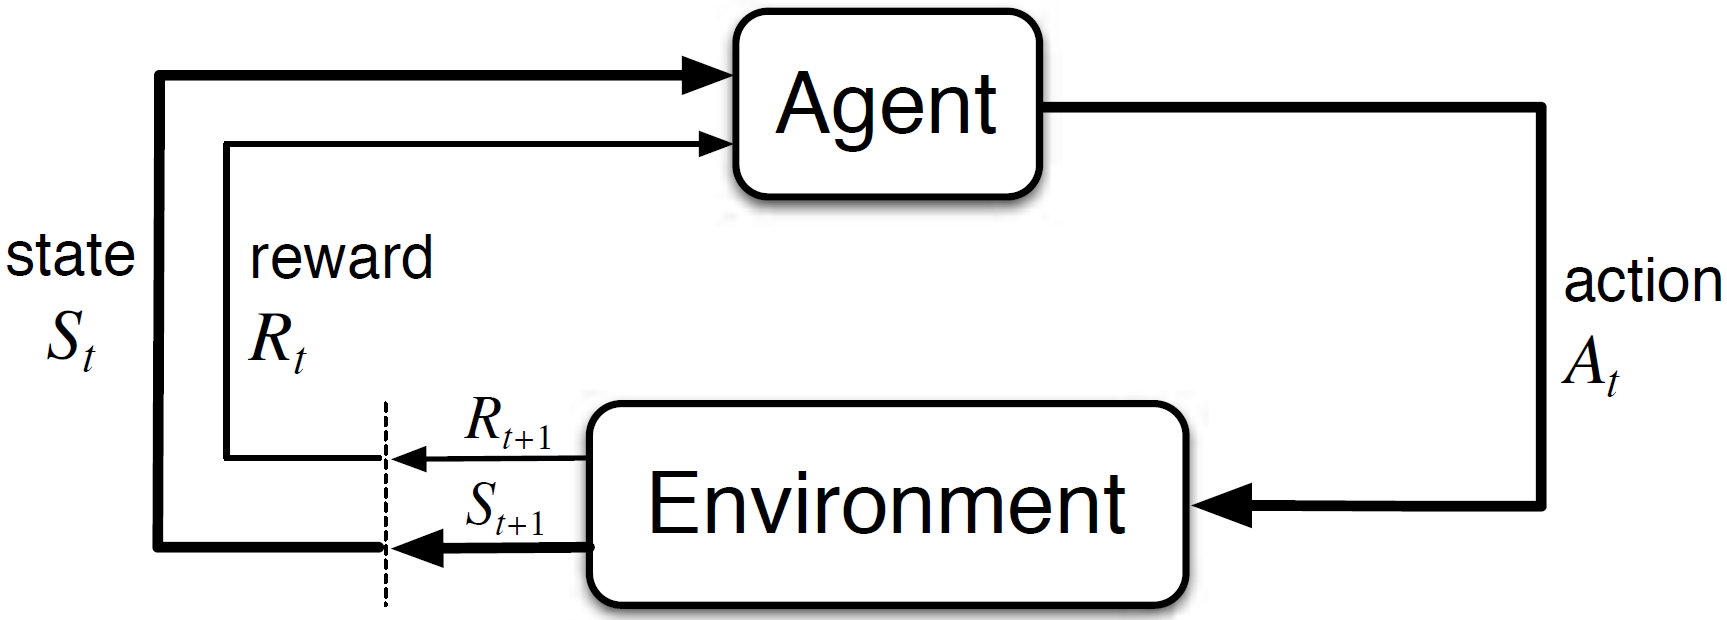
\includegraphics[scale=0.2]{04_Artefakte/01_Abbildungen/rl/rl_agent_environment_interaction.png}
    \caption[Modell der Interaktion zwischen Agent und Umgebung in einem \acs{MDP}]{Modell der Interaktion zwischen Agent und Umgebung (\engl Environment) in einem \acs{MDP} \protect\footnotemark}
    \label{fig:rl_agent_environment_interaction}
\end{figure}
\footnotetext{Abbildung entnommen aus \cite[S. 47]{suttonReinforcementLearningIntroduction2018}}

Zur Modellierung der Umgebung und deren Dynamik können \ac{MDP} genutzt werden. \ac{MDP} basieren auf  Markov Ketten und gehören zum Gebiet der mathematischen Optimierung. Ein \ac{MDP} ist definiert als ein Tupel $(S,A,p,r)$ \cite[S. 47ff.]{suttonReinforcementLearningIntroduction2018}, \cite[S. 5]{kontesg.SeminarReinforcementLearning2021}:
\begin{itemize}
    \item $S$ = Menge von Zuständen $s$
    \item $A$ = Menge möglicher Aktionen $a$
    \item $p(s' \mid s,a) = Pr(S_{t+1}=s' \mid S_{t}=s, A_{t}=a)$ für das gilt: $\sum_{a\in A}p(s'\mid s,a) =1$ \\ State-Transition Probability 
    \item $r(s,a) \rightarrow \mathbb{R}$ Rewardfunktion
\end{itemize}

Die Dynamik der Zustandsübergänge wird modelliert durch die State-Transition Probability $p$ (\dt Zustandsübergangs Wahrscheinlichkeit). 
Sie beschreibt die Wahrscheinlichkeit, bei Wahl von Aktion $a$ im Zustand $s$ in den Folgezustand $s'$ überzugehen.
Die State-Transition Probability ist als Wahrscheinlichkeitsverteilung definiert, da die Zustandsübergänge nicht deterministisch sein können. 
%Die Wahl von Aktion $a$ in Zustand $s$ kann in unterschiedlichen Folgezuständen $s'$ resultieren. 
%Die einzige Ausnahme sind Terminalzustände $S_T$, die per Definition ihr eigener Folgezustand sind \cite[S. S. 47]{suttonReinforcementLearningIntroduction2018}: $p(s \mid s,a)=1, \forall a \in A \mid S_T =s$

Zudem definiert die State-Transition Probability, dass der Folgezustand $s'$ nur vom Zustands $s$ und der darin gewählten Aktion $a$ abhängig ist. 
Zuvor besuchte Zustände oder gewählte Aktionen müssen zur Berechnung des Folgezustands nicht bekannt sein und sind implizit im Zustand $s$ enthalten. Dies wird als Markov Eigenschaft bezeichnet und ist Voraussetzung dafür, dass ein Problem als ein \ac{MDP} formuliert werden kann. \cite[S. 66]{suttonLearningPredictMethods1988}

Nach jeder Aktion des Agenten verteilt die Umgebung abhängig vom aktuellen Zustand einen Reward gemäß der Rewardfunktion. 
Die Rewardfunktion definiert das Ziel, das der Agent erreichen soll, da dieser den kumulierten Reward maximiert.
Der kumulierte Reward, den der Agent ausgehend vom Zeitschritt $t$ erhält, wird als Return $G_t$ bezeichnet. 
Für episodische Probleme ist der Return definiert als \cite[S. 54]{suttonReinforcementLearningIntroduction2018}:

\begin{equation}
    \label{eq:return_episodic}
    \equationentry{Berechnung Return $G_t$ für episodische Probleme}
    G_t=R_{t+1}+R_{t+2}+...+R_T
\end{equation}

Für Markov-Prozesse mit einer unendlichen Dauer. \dahe eine diskrete, unendliche Markov-Kette, ist $G_t$ eine unendliche Reihe, für die zur Berechnung ein Diskontierungsfaktor  $0 \le \gamma \le 1$ notwendig ist
Der Diskontierungfaktor kann auch auf episodische Probleme angewandt werden, um das Verhalten des Agenten zu beeinflussen. 
Für $\gamma=0$ beträgt $G_t= R_{t+1}$, sodass der Agent nur den direkten Reward maximiert. 
Hingegen beachtet der Agenten die späteren Rewards mit steigendem $\gamma$ mehr. \cite[S. 55f.]{suttonReinforcementLearningIntroduction2018}

\begin{equation}
    \label{eq:return_continuous}
    \equationentry{Berechnung Return $G_t$ für Probleme unendlicher Zeitdauer}
    G_t=R_{t+1}+\gamma R_{t+2}+\gamma^2R_{t+3} + \dots =\sum_{k=0}^{\infty}\gamma^{k}R_{t+k+1}
\end{equation}

Da ein Return $G_t$ den darauf folgenden Return $G_{t+1}$ enthält, kann \cref{eq:return_continuous} umgeformt werden in \cref{eq:return_nextstate}, um diese Beziehung zu verdeutlichen. Diese Beziehung aufeinander folgender Returns ist die Basis vieler \ac{RL} Methoden. \cite[S. 54 f.]{suttonReinforcementLearningIntroduction2018}

\begin{equation}
    \label{eq:return_nextstate}
    \equationentry{Beziehung aufeinander folgender Returns}
     G_t= R_{t+1}+\gamma R_{t+2}+\gamma^2R_{t+3} +\dots = R_{t+1}+\gamma(R_{t+2}+\gamma R_{t+3} +  \dots) = R_{t+1}+\gamma G_{t+1}
\end{equation}

 
Ein Beispiel für ein \ac{RL} Problem, das als \ac{MDP} modelliert werden kann, ist die sogenannte \gqq{Gridworld} in \cref{fig:gridworld_blank}. 
Der Agent startet im Feld $C1$ und soll lernen das Feld A4 zu erreichen. 
Der Zustandsraum sind die einzelnen Felder, die der Agent betreten kann. 
Das Feld B2 repräsentiert ein Hindernis und zählt nicht zum Zustandsraum. 
Die Felder A4 und B4 sind Terminalzustände. 
In jedem Zustand wählt der Agent als Aktion eine Himmelsrichtung, in der er sich bewegen möchte. Somit umfasst der Aktionsraum für jeden Zustand: Norden, Westen, Süden und Osten. 
Bei einer Bewegung in Richtung Wand oder dem Hindernis B2 verbleibt der Agent im gleichen Feld. 
Die Zustandsübergänge sind nicht deterministisch. 
Wählt der Agent eine Richtung aus, bewegt er sich nur mit einer Wahrscheinlichkeit von 80\% dorthin. 
Es besteht eine Wahrscheinlichkeit von je 10\%, dass sich der Agent in eine der angrenzenden Richtungen bewegt. 
Die Rewardfunktion definiert das Ziel des Agenten. 
Erreicht der Agent das Feld A4 erhält er einen Reward von $+1$. 
Hingegen erhält er im Agent beim Erreichen des Feldes B4 eine Bestrafung von $-1$. 
Der direkt Reward für jeden anderen Zustandsübergang des Agenten beträgt $-0,1$.
Da der Agent den Return maximiert, versucht er dadurch das Ziel in möglichst wenigen Zustandsübergängen zu erreichen. \cite[S. 10 ff.]{kontesg.SeminarReinforcementLearning2021}

\begin{figure}
    \centering
    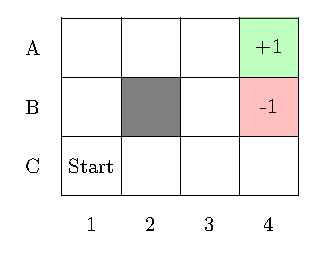
\includegraphics{gridworld/gridworld_blank.pdf}
    \caption[Aufbau des \gqq{Gridworld} Problems]{Aufbau des \gqq{Gridworld} Problems. Agent startet im Feld C1. Die Felder A4 und B4 sind Terminalzustände. B2 ist ein Hindernis.\protect\footnotemark}
    \label{fig:gridworld_blank}
\end{figure}
\footnotetext{eigene Darstellung in Anlehnung an \cite[S. 10ff.]{kontesg.SeminarReinforcementLearning2021}}

\subsection{Policy und State-Value Funktion}
\label{sec:policy_statevalue}

Der Return $G_t$ ist abhängig von den Aktionen, die der Agent in jedem Zustand wählt. 
Die Strategie, nach der Aktionen gewählt werden, wird als Policy $\pi$ bezeichnet.
Eine Policy $\pi$ ist eine Funktion $\pi(a \mid s)$, die für alle Zustände $s \in S$ die Wahrscheinlichkeit definiert, dass der Agent eine Aktion $a \in A$ wählt. 
Somit beschreibt eine Policy das Verhalten eines Agenten in jedem Zustand. 
Eine Policy kann stochastisch $\pi(a \mid s)$ oder deterministisch $\pi (s)$ sein. \cite[S. 58]{suttonReinforcementLearningIntroduction2018}

Auf der Basis einer Policy kann jedem Zustand ein Wert zugewiesen werden, der als State-Value (\dt Zustandswert) bezeichnet wird. 
Der State-Value ist der Erwartungswert des Return $G_t$, wenn der Agent im Zustand $s$ der Policy $\pi$ bis zum Ende der Episode folgt. 
Diese Abbildung von Zustand auf State-Value ist die State-Value Funktion:

\begin{equation}
    \label{eq:statevalue_function}
    \equationentry{Definition State-Value Funktion}
    v_{\pi}(s)=\mathbb{E}[G_t|S_t=s]
\end{equation}

Die State-Value Funktion kann mittels \cref{eq:return_nextstate} als Return aufeinander folgender Zeitschritte und somit aufeinander folgender State-Value Funktionen umgeformt werden:

\begin{equation}
    \label{eq:statevalue_relation}
    \equationentry{Beziehung zwischen State-Value Funktionen aufeinander folgender Zeitschritte}
    v_{\pi}(s)=\mathbb{E}_\pi[G_t|S_t=s] = \mathbb{E}_\pi[R_{t+1}+\gamma G_{t+1}]= R_{t+1} + \gamma \mathbb{E}[G_{t+1} \mid S_{t+1}=s']=R_{t+1}+v_\pi(s')
\end{equation}

\cref{fig:gridworld_policy_statevalue} zeigt für das Beispiel Gridworld eine mögliche deterministische Policy und die dazugehörige Zuweisung von State-Values. Ein Pfeil symbolisiert die Aktion, die der Agent gemäß Policy im jedem Zustand wählt. Zur Berechnung der State-Values wurde die oben beschriebene Rewardfunktion und ein Diskontierungsfaktor $\gamma=0,9$ verwendet.


\begin{figure}
    \centering
    \begin{subfigure}[b]{0.45\textwidth}
      \centering
      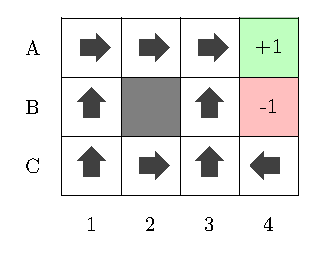
\includegraphics[]{gridworld/gridworld_policy.pdf}
      \caption{Mögliche Policy $\pi$}
      \label{fig:gridworld_policy}
    \end{subfigure}
    \begin{subfigure}[b]{0.45\textwidth}
      \centering
      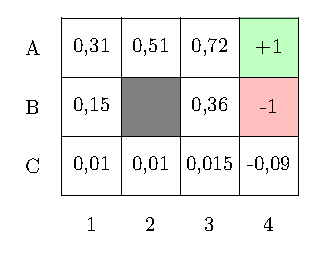
\includegraphics[]{gridworld/gridworld_statevalues.pdf}
      \caption{State-Values zur Policy $\pi$ aus (a)}
      \label{fig:gridworld_statevalues}
    \end{subfigure}
    \caption[Policy und State-Value für das Beispiel Gridworld]{Policy und State-Value für das Beispiel Gridworld\protect\footnotemark}
    \label{fig:gridworld_policy_statevalue}
    
\end{figure}
\footnotetext{eigene Darstellung in Anlehnung an \cite[S. 75.]{kontesg.SeminarReinforcementLearning2021}}

Die State-Value Funktion ermöglicht den Vergleich von Policies.
Eine Policy $\pi$ ist besser als eine andere Policy $\pi'$ wenn ihre zugehörige State-Value Funktion für alle Zustände $s$ einen größeren Wert hat, als die Policy $\pi'$: $v_\pi(s) \ge v_{\pi'}(s) \forall s \in S$

Es kann mindestens eine Policy geben, die besser als alle anderen Policies oder gleich gut ist.
Diese Policy wird als optimale Policy $\pi_*$ bezeichnet und die zugehörige Value Funktion als optimale State-Value Funktion $v_*$. \cite[S. 61 ff.]{suttonReinforcementLearningIntroduction2018}
Eine Policy ist optimal, wenn der Return $G_t$ für jeden Zustand $s \in S$ den maximal möglichen Wert annimmt.
Somit ist die optimale Policy $\pi_*$ die Lösung für den \ac{MDP} und das darin formulierte \ac{RL} Problem \cite[S. 62 ff.]{suttonReinforcementLearningIntroduction2018}.
Ist für einen \ac{MDP} das Tupel $(S,A,p,r)$ gegeben, kann die optimale Policy durch Dynamic Programming ermittelt werden. Beim Dynamic Programming wird ein Gleichungssystem aufgestellt und durch iteratives Verbessern der Policy und State-Value Funktion gelöst.\cite[S. 73ff.]{suttonReinforcementLearningIntroduction2018} 
\section{Temporal-Difference Learning}
Dieser Abschnitt behandelt das \ac{RL} Teilgebiet des \acl{TDL} (\ac{TDL}).
Zunächst wird das Konzept von \ac{TDL} am Beispiel von \ac{TD} Prediction erklärt. 
Anschließend werden die darauf basierenden \ac{TD} Algorihtmen \bothAlgs vorgestellt und miteinander verglichen.

\subsection{Temporal-Difference Prediction}
\label{sec:td_prediction}

Wenn ein \ac{RL} Problem als ein \ac{MDP} beschrieben werden kann, aber die State-Transition Probability oder die Rewardfunktion nicht bekannt sind, kann kein Modell der Umgebung erstellt werden. 
Folglich lassen sich diese \ac{RL} Probleme nicht mittels Dynamic Programming lösen. 
\ac{TDL} ist ein Teilgebiet von \ac{RL}, das Methoden definiert, die kein Modell der Umgebung und ihrer Dynamik benötigen. 
Stattdessen lernen \ac{TD} Methoden direkt durch Interaktion mit der Umgebung.
\ac{TDL} gilt daher als einer der zentralen Meilensteine von \ac{RL} und \ac{TD} Methoden werden als modellfreies RL bezeichnet \cite[S. 119]{suttonReinforcementLearningIntroduction2018}.
Die Voraussetzung zur Anwendung von \ac{TDL} ist, dass der Agent wie in \cref{formalisierung} beschrieben mit der Umgebung gemäß einer Policy $\pi$ interagieren kann \cite[S.88, S. 94]{kontesg.SeminarReinforcementLearning2021}. 

Von der Umgebung erhält der Agent seinen aktuellen Zustand $S_t$ und nach einer Aktion $A_t$ im nächsten Zeitschritt den Folgezustand $S_{t+1}$ und Reward $R_{t+1}$. 
Das Tupel $(S_t, A_t, S_{t+1}, R_{t+1})$ ist ein Sample (\dt Probe) von der Umgebung. 
Auf Basis der Samples schätzt \ac{TD} Prediction die zur Policy $\pi$ zugehörige State-Value Funktion $v_\pi$.
Der Schätzwert der State-Value-Funktion $V$ wird zu Beginn für jeden Zustand willkürlich initialisiert. \cite[S. 120f.]{suttonReinforcementLearningIntroduction2018}

Das Schätzen der State-Value Funktion durch Interaktion ist möglich aufgrund der in \cref{eq:statevalue_relation} definierten Beziehung zwischen State-Values aufeinander folgender Zeitschritte. 
Nach dieser Gleichung ist der exakte Wert der State-Value Funktion unter Policy $\pi$ eines Zustands $S_t$ der direkte Reward $R_{t+1}$ und der State-Value des Folgezustands $S_{t+1}$. \cite[S. 120f.]{suttonReinforcementLearningIntroduction2018}

\begin{equation}
    \equationentry{Beziehung zwischen State-Value Funktionen}
    v_{\pi}(S_t)= R_{t+1}+v_\pi(S_{t+1})
\end{equation}

Da in einem Sample der Zustand, Reward und Folgezustand enthalten sind, kann der State-Value für den Zustand $S_t$ auf Basis des darauffolgenden Zeitschritts geschätzt werden. 
Dieser Schätzwert für $V(S_t)$ wird als \ac{TD} Target bezeichnet. \cite[S. 120f.]{suttonReinforcementLearningIntroduction2018}

\begin{equation}
    \label{eq:td_target}
    \equationentry{Temporal-Difference Target}
    V(S_t)= R_{t+1}+\gamma V(S_{t+1})
\end{equation}

Da das \ac{TD} Target den Reward aus der Umgebung enthält, ist es ein besserer Schätzwert für $S_t$ als der willkürlich initialisierte Schätzwert $V(S_t)$. 
Die Differenz zwischen beiden Schätzwerten wird als \ac{TD} Error $\delta_t$ bezeichnet. 
Der \ac{TD} Error beschreibt den Unterschied zwischen zwischen dem alten und neuen Schätzwert und somit wie gut die alte Schätzung war. \cite[S. 120f.]{suttonReinforcementLearningIntroduction2018}

\begin{equation}
    \label{eq:td_error}
    \equationentry{Temporal-Difference Error}
    \delta_t = R_{t+1} + \gamma V(S_{t+1}) - V(S_t)
\end{equation}

Da das \ac{TD} Target ein besserer Schätzwert für $S_t$ ist, muss der Schätzwert $V(S_t)$ in Richtung des \ac{TD} Target korrigiert werden. 
Diese Aktualisierung ist das \ac{TD} Update und ein exponentiell geglätteter Mittelwert. \cite[S. 33]{suttonReinforcementLearningIntroduction2018}
\cref{eq:td_update} zeigt die Formel für das \ac{TD} Update. 
Im \ac{TD} Update wird der alte Schätzwert gemäß einer Lernrate $\alpha$ aktualisiert, die die Gewichtung des \ac{TD} Error festlegt. \cite[S. 120]{suttonReinforcementLearningIntroduction2018}

\begin{equation}
    \label{eq:td_update}
    \equationentry{Temporal-Difference Update}
    V(S_t) \leftarrow V(S_t) + \alpha [R_t+\gamma V(S_{t+1}) -V(S_t)]
\end{equation}

Um die State-Value Funktion für alle Zustände $S$ zu schätzen, interagiert der Agent wiederholt über mehrere Episoden mit der Umgebung. 
Nach jedem Zeitschritt führt der Agent für den im vorherigen Zeitschritten besuchten Zustand das \ac{TD} Update durch. 
Dieser Ablauf bildet die Grundlage für alle \ac{TD} Methoden. \cite[S. 121]{suttonReinforcementLearningIntroduction2018}
In \cite{suttonLearningPredictMethods1988} und \cite{watkinsQlearning1992} wurde bewiesen, dass \ac{TD} Prediction zur wirklichen State-Value Funktion $v_\pi$ konvergiert. 
Dafür müssen zwei Bedingungen erfüllt werden. 
Zum einen müssen alle Zustände hinreichend oft besucht werden. 
Zum anderen muss die im \ac{TD} Update genutzte Lernrate $\alpha$ hinreichend klein sein oder im Laufe des Trainings abnehmen. \cite[S. 33, S. 124]{suttonReinforcementLearningIntroduction2018}, \cite[S. 285 f.]{watkinsQlearning1992}

Am Beispiel von Gridworld aus \cref{sec:policy_statevalue} soll das \ac{TD} Update durchgeführt werden. 
Die Rewardfunktion und State-Transition Probability sind unverändert, dem Agenten jedoch nicht bekannt. 
In \cref{fig:gridworld_tdl} wird die zu untersuchende Policy dargestellt.
Die State-Values aller Zustände werden mit 0 initialisiert. 
Der blaue Pfeil zeigt die Zustandsübergänge des Agenten in der ersten Episode. 
Rechts neben der Abbildung ist das \ac{TD} Update mit Lernrate $\alpha=0,1$ und Diskontierungsfaktor $\gamma=0,9$ für den Zustand A3. 
Das \ac{TD} Update wird im darauf folgenden Zeitschritt durchgeführt und somit nachdem der Agent das Ziel A4 erreicht hat.

\begin{figure}
   \begin{minipage}[c]{.5\textwidth}
   \centering
    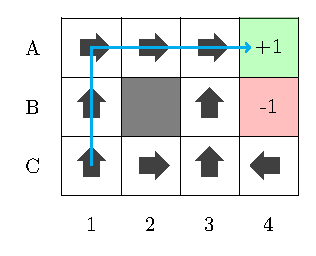
\includegraphics[]{gridworld/gridworld_tdl.pdf}
   \end{minipage}%
   \begin{minipage}[c]{.5\textwidth}
    $V(A3) \leftarrow V(A3)+ \alpha[R+\gamma V(A4)-V(A3)]\\
V(A3) = 0+0,1[-0,1+0,9 \cdot 1-0]=0,1$
   \end{minipage}
   \caption[\acs{TD} Update am Beispiel von Gridworld]{\acs{TD} Update am Beispiel von Gridworld. Der blaue Pfad zeigt den Pfad es Agenten in der ersten Episode. Rechts wird das \ac{TD} Update für den Zustand A3 berechnet. \protect\footnotemark}
   \label{fig:gridworld_tdl}
\end{figure}
\footnotetext{eigene Darstellung in Anlehnung an \cite[S. 99]{kontesg.SeminarReinforcementLearning2021}}
\subsection{\sarsa}
Der \ac{TD} Algorithmus Sarsa verwendet das Konzept von \ac{TD} Prediction, um die optimale Policy $\pi_*$ zu ermitteln. 
Statt der State-Value Funktion $v_\pi$ approximiert Sarsa die Action-Value Funktion $q_\pi$. 
Der Schätzwert der Action-Value Funktion $q_\pi$ ist $Q$. \cite[S. S. 129]{suttonReinforcementLearningIntroduction2018}
Die Action-Value Funktion $q_\pi(s,a)$ weist \ac{SA Tupel} einen \qValue zu. 
Der \qValue ist der kumulierte Reward, den der Agent erwarten kann, wenn er im Zustand $s$ die Aktion $a$ wählt und danach der Policy $\pi$ folgt. 
Für die Action-Value Funktion gilt daher auch die Beziehung aufeinander folgender Returns, sodass das \ac{TD} Update wie folgt formuliert werden kann \cite[S. 129f.]{suttonReinforcementLearningIntroduction2018}:

\begin{equation}
    \label{eq:sarsa_update}
    \equationentry{TD Update Sarsa}
    Q(S_t,A_t) \leftarrow Q(S_t,A_t) +\alpha[R_{t+1} + \gamma Q(S_{t+1},A_{t+1})-Q(S_t,A_t)]
\end{equation}

Um das Update durchführen benötigt Sarsa das Tupel $(S_t,A_t,R_{t+1},S_{t+1},A_{t+1})$, was der Ursprung für den Namen des Algorithmus ist. 
Auf Basis der Update-Regel kann Sarsa eine Schätzung $Q$ der Action-Value Funktion zur Policy $\pi$ aufstellen, nach der Sarsa mit der Umgebung interagiert. \cite[S. 129f.]{suttonReinforcementLearningIntroduction2018}
Der Agent verwaltet die Abbildung von \ac{SA Tupel} auf ihren geschätzten \qValue in einer \qtable. 
Mittels dieser kann Sarsa für jeden Zustand die Aktion ermitteln, die im höchsten \qValue resultiert.
Da Sarsa die \qValues mit jeder neuen Episode aktualisiert, kann Sarsa zur Interaktion mit der Umgebung einer Greedy-Policy folgen.
Bei einer Greedy-Policy wird immer die Aktion gewählt, die den höchsten \qValue hat.\footnote{Gibt es mehrere Aktionen mit dem höchsten\qValue, wird willkürlich eine der Aktionen gewählt}
Dadurch wird iterativ die Action-Value Funktion verbessert und die Policy nähert sich optimalen Policy $\pi_*$. \cite[S. 129f.]{suttonReinforcementLearningIntroduction2018}

Würde Sarsa ausschließlich gemäß einer Greedy-Policy mit der Umgebung interagieren, könnte der Agent in lokalen Maxima verweilen und würde nicht die optimale Policy lernen. 
Eine mögliche Lösung ist die $\epsilon$-greedy-Policy. 
Die $\epsilon$-greedy-Policy wählt mit einer Wahrscheinlichkeit von $\epsilon$ eine zufällige Aktion und $1-\epsilon$ die Aktion mit dem höchsten \qValue.
Der Hyperparameter $\epsilon$ ist die Explorationswahrscheinlichkeit. \cite[S. 28f.]{suttonReinforcementLearningIntroduction2018}

Damit Sarsa zur optimalen Policy $\pi_*$ konvergiert, muss neben den Konvergenzbedingungen von TD Prediction das Epsilon während dem Training gegen 0 konvergieren \cite[S. 129]{suttonReinforcementLearningIntroduction2018}. 
Bei der Wahl der Explorationswahrscheinlichkeit $\epsilon$ muss eine Balance zwischen Exploration und Exploitation, \dahe Ausnutzung der Aktionen mit höchsten \qValue, ermittelt werden. 
Das Abwägen beider Aspekte wird als Explorations-Exploitations-Dilemma bezeichnet \cite[S. 3]{suttonReinforcementLearningIntroduction2018}.

Der Ablauf des Sarsa Algorithmus ist als Pseudocode formuliert in Algorithmus \ref{algo_sarsa}.\footnote{eigene Darstellung in Anlehnung an \cite[S. 130]{suttonReinforcementLearningIntroduction2018}}

{\centering
\begin{minipage}{0.7\textwidth}
\begin{algorithm}[H]
\SetAlgoLined
\DontPrintSemicolon
\SetKwInput{kwAlgorithmParam}{Algorithm parameters}
\kwAlgorithmParam{step size $\alpha \in (0;1]$, small $\epsilon > 0$}
Initialize $Q(s,a)$, for all $s \in S^+, a \in A(s)$, arbitrarily except that $Q(terminal,\cdot)=0$\;
\BlankLine
\ForEach{episode}{
    Initialize $S$\;
    Choose $A$ from $S$ using policy derived from $Q$ (e.g., $\epsilon$-greedy)\;
    \ForEach{step of episode}{
        Take action $A$, observe $R$, $S'$\;
        Choose $A'$ from $S'$ using policy derived from $Q$ (e.g., $\epsilon$-greedy)\;
        $Q(S,A) \leftarrow Q(S,A) + \alpha[R+\gamma Q(S',A')-Q(S,A)]$\;
        $S \leftarrow S'; A \leftarrow A';$
    }
}
\caption{Sarsa}
\label{algo_sarsa}
\end{algorithm}
\end{minipage}
\par
}
\subsection{\qlearning}
Q-Learning lernt ebenfalls die optimale Policy durch Schätzung der Action-Value Funktion. 
Im Gegensatz zu Sarsa approximiert Q-Learning jedoch direkt die optimale Action-Value Funktion $q_*$ und somit die optimale Policy $\pi_*$.
Dafür nutzt Q-Learning bei der Aktualisierung seines Schätzwertes $Q(S_t,A_t)$ immer die Aktion $a$ des Folgezustands $S_{t+1}$, die den maximalen $Q$-Value hat.   
Dies ist  unabhängig davon welche Aktion $A_{t+1}$ der Agent schlussendlich ausführt.  \cite[S. 177]{watkinsLearningDelayedRewards1989} 
Das Update für Q-Learning kann daher wie in \cref{eq:ql_update} formuliert werden\cite[S. 131]{suttonReinforcementLearningIntroduction2018}.

\begin{equation}
    \label{eq:ql_update}
    \equationentry{TD Update Sarsa}
    Q(S_t,A_t)\leftarrow Q(S_t,A_t)+\alpha[R_{t+1}+\gamma\max_aQ(S_{t+1},a)-Q(S_t,A_t)]
\end{equation}

Die Policy $\pi$, die zur Interaktion mit der Umgebung genutzt wird, ist jedoch dennoch wichtig, da sie entscheidet welche Samples der Agent erhält. 
Da für die Aktualisierung jedoch immer der maximale Q-Value genutzt wird, ist eine Abnahme der Explorationswahrscheinlichkeit bei Nutzung von $\epsilon$-greedy keine Bedingung für die Konvergenz zur optimalen Policy \cite[S. 131f.]{suttonReinforcementLearningIntroduction2018}.
Wenn die Konvergenzbedingungen von \ac{TD} Prediction eingehalten werden, ist Q-Learning garantiert zur optimalen Policy $\pi_*$ zu konvergieren \cite[S. 286]{watkinsQlearning1992}.

Der Ablauf des Q-Learning Algorithmus ist als Pseudocode formuliert in Algorithmus \ref{algo_qlearning}.\footnote{eigene Darstellung in Anlehnung an \cite[S. 131]{suttonReinforcementLearningIntroduction2018}}

{\centering
\begin{minipage}{0.7\textwidth}
\begin{algorithm}[H]
\SetAlgoLined
\DontPrintSemicolon
\SetKwInput{kwAlgorithmParam}{Algorithm parameters}

\kwAlgorithmParam{step size $\alpha \in (0;1]$, small $\epsilon > 0$}
Initialize $Q(s,a)$, for all $s \in S^+, a \in A(s)$, arbitrarily except that $Q(terminal,\cdot)=0$\;
\BlankLine
\ForEach{episode}{
    Initialize $S$\;
    \ForEach{step of episode}{
        Choose $A$ from $S$ using policy derived from $Q$ (e.g., $\epsilon$-greedy)\;
        Take action $A$, observe $R$, $S'$\;
        $Q(S,A) \leftarrow Q(S,A) + \alpha[R+\gamma \max_{a} Q(S',a)-Q(S,A)]$\;
        $S \leftarrow S'$
    }
}
\caption{Q-Learning}
\label{algo_qlearning}
\end{algorithm}
\end{minipage}
\par
}



\subsection{Vergleich von \bothAlgs}
\label{chap:vergleich}

Die Algorithmen \bothAlgs haben zwei zentrale Unterschiede. 
Zum einen die Aktion des Folgezustands und somit der Q-Value, der für das Update genutzt wird. 
Zum anderen der Zeitpunkt, zu dem das Update durchgeführt wird \cite{IrelandComparisonThereFundamental}. 
Sarsa nutzt für das Update die Aktion, die es gemäß seiner Policy auswählt. 
Hingegen nutzt Q-Learning für das Update immer die Aktion mit dem höchsten Q-Value, auch wenn es gemäß Policy eine andere Aktion ausführt. 
Aufgrund dessen wird Sarsa als ein On-Policy und Q-Learning als ein Off-Policy Algorithmus klassifiziert \cite[S. 132]{suttonReinforcementLearningIntroduction2018}.

Zur Veranschaulichung des Unterschiedes wird das Update von Sarsa und Q-Learning am Beispiel von Gridworld erklärt. 
\cref{fig:gridworld_sample} zeigt die $\epsilon$-greedy-Policy, nach der beide Agent mit der Umgebung interagieren. 
Die State-Transition Probability und Rewardfunktion sind unverändert, aber den Agenten nicht bekannt.
Es gilt $\gamma=0,9$ und $\alpha=0,1$.
Der blaue Pfeil zeigt den Pfad einer Episode für beide Agenten. 
\cref{tab:tdlexample} enthält einen Ausschnitt einer willkürlich gefüllten Q-Tabelle für die Zustände C1 und C2.

\begin{minipage}{\textwidth}
  \begin{minipage}[b]{0.49\textwidth}
    \centering
    \captionsetup{type=figure}
    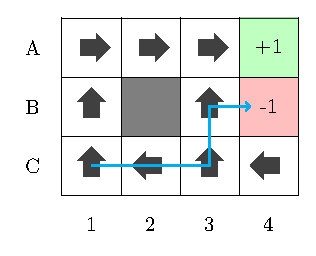
\includegraphics[]{gridworld/gridworld_sample.pdf}
    \captionof{figure}[Sample Episode für Gridworld]{Sample Episode für Gridworld\protect\footnotemark}
    \label{fig:gridworld_sample}
  \end{minipage}
  \hfill
  \begin{minipage}[b]{0.49\textwidth}
    \centering
    \captionsetup{type=table}
    % \begin{table}
\begin{tabular}{llr}
\toprule
Zustand $S$ & Aktion $A$    & $Q(S,A)$ \\ \midrule
C1          & Norden        & 10,5     \\
            & Westen        & 5,0      \\
            & Süden         & 8,7      \\
            & Osten         & 0,1      \\ \cmidrule{1-3}
C2          & Norden        & 8,2      \\ 
            & Westen        & -2,0     \\
            & Osten         & 9,8      \\
            & Süden         & 6,5      \\ \bottomrule
\end{tabular}
% \end{table}
% \begin{table}
% \centering
% \caption{\qtable mit Beispieleinträgen für Gridworld}
% \label{tab:qtable_tdl_example}

% \begin{tabular}{llr}
% \toprule
% Zustand $S$ & Aktion $A$    & $Q(S,A)$ \\ \midrule
% C1          & Norden        & 10,5     \\
%             & Westen        & 5,0      \\
%             & Süden         & 8,7      \\
%             & Osten         & 0,1      \\ \cmidrule{1-3}
% C2          & Norden        & 8,2      \\ 
%             & Westen        & -2,0     \\
%             & Osten         & 9,8      \\
%             & Süden         & 6,5      \\
% $\vdots$    & $\vdots$      & $\vdots$ \\ \bottomrule
% \end{tabular}
% \end{table}
    \captionof{table}{Willkürlich gefüllte \qtable für Gridworld}
    \label{tab:tdlexample}
    \end{minipage}
\end{minipage}
\footnotetext{eigene Darstellung in Anlehnung an \cite[S. 127]{kontesg.SeminarReinforcementLearning2021}}

Im Zustand C1 wählt der Agent die Greedy-Aktion “Norden”. Wegen der Transposition-Probability wechselt der Agent jedoch in den Zustand C2. Im Zustand C2 ist die Greedy-Aktion “Osten”. Der Agent wählt aufgrund von $\epsilon$-greedy zufällig die Aktion “Westen”. Das Sample $(S_t,A_t,R_{t+1},S_{t+1},A_{t+1})$ der Umgebung ist somit: $(C1;N;-0,1;C2;W)$ 

Der Sarsa-Agent führt das Update in \cref{eq:sarsa_update_example} durch. Hingegen wählt der Q-Learning Agent für den Folgezustand die Aktion mit höchstem Q-Value $Q(C2,Osten)=9,8$ führt daher das Update aus \cref{eq:ql_update_example} durch.

\begin{equation}
    \label{eq:sarsa_update_example}
    \equationentry{Beispiel TD Update Sarsa}
    \begin{split}
    Q(C1,N) & =Q(C1,N)+\alpha[-0,01+0,09Q(C2, W)-Q(C1,N)] \\
    Q(C1,N) & =10,5+0,1[-0,1+0.9(-2,0)-10.5]=9,26
    \end{split}
\end{equation}

\begin{equation}
    \label{eq:ql_update_example}
    \equationentry{Beispiel TD Update Q-Learning}
    \begin{split}
        Q(C1,N) &=Q(C1,N)+\alpha[-0,01+0,09Q(C2, O)-Q(C1,N)]\\
        Q(C1,N) &=10,5+0,1[-0,1+0.9(9,8)-10.5]=10,32
    \end{split}
\end{equation}



Würden beide Algorithmen einer Greedy-Policy folgen, wäre das Update gleich. 
Während Sarsa seine Aktion $A_{t+1}$ vor dem Update ausgewählt hat, wählt Q-Learning diese erst, nachdem das Update durchgeführt wurde. 
In Situationen, in denen ein Zustand der eigene Folgezustand ist, könnten Q-Learning und Sarsa unterschiedliche Aktionen $A_{t+1}$ auswählen, da sich die \qValues der Aktionen durch das Update geändert haben könnten. \cite{IrelandComparisonThereFundamental}

Ein weiteres Beispiel, dass den Unterschied von Q-Learning und Sarsa verdeutlicht ist \gqq{Cliff Walking} in \cref{fig:cliffwalking}. 
Bei diesem soll ein Agent vom Startbereich “S” zum Ziel “G” laufen. 
In jedem Zeitschritt erhalten die Agenten einen Reward $-1$, sodass sie das Ziel möglichst schnell erreichen sollen. 
Betritt ein Agent den Bereich Klippe, erhält dieser einen Reward von $-100$. 
Die Agenten können sich wieder in alle vier Himmelsrichtungen bewegen. 
Im Gegensatz zur Gridworld sind die Zustandsübergänge deterministisch. 
Die Algorithmen Q-Learning und Sarsa lernen beide mittels einer $\epsilon$-greedy-Policy mit konstantem $\epsilon$=0,1. 
Die Abbildung zeigt den optimalen Pfad (rot) und den sicheren Pfad (blau), der einen geringeren Return erzielt, aber mit größerer Wahrscheinlichkeit im Ziel ankommt. 
Während des Trainings lernt Q-Learning den optimalen Pfad, betritt jedoch aufgrund von $\epsilon=0,1$ regelmäßig die Klippe. 
Hingegen lernt Sarsa den sicheren Pfad, da es im Update die aktuelle Policy beachtet. 
Konvergiert $\epsilon$ während dem Training gegen 0 lernt Sarsa ebenfalls den optimalen Pfad. \cite[S. 132]{suttonReinforcementLearningIntroduction2018}

\begin{figure}[h]
    \centering
    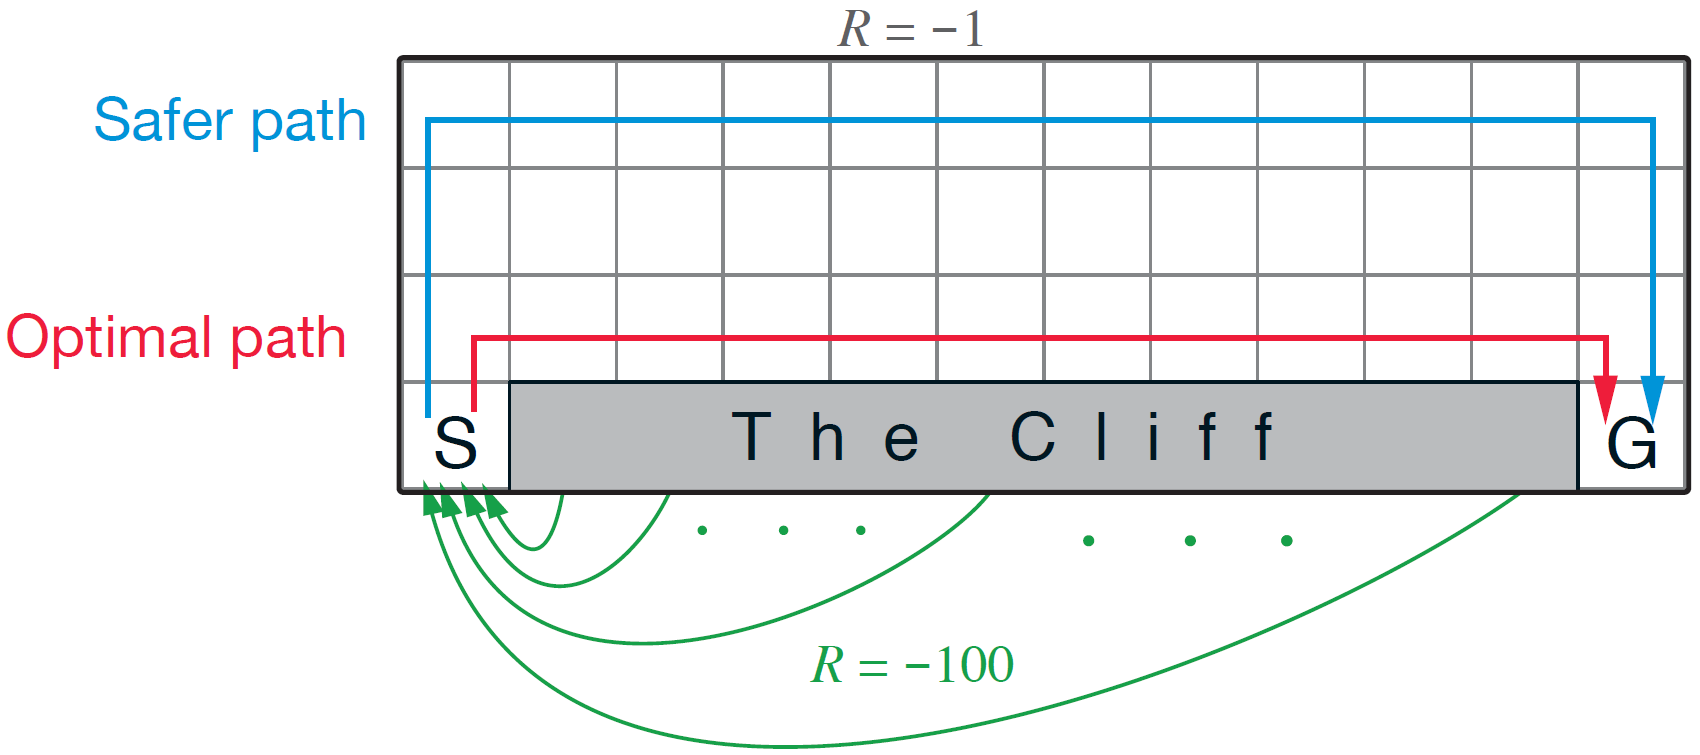
\includegraphics[scale=0.2]{04_Artefakte/01_Abbildungen/rl/rl_cliff_environment.png}
    \caption[Cliff Walking]{Cliff Walking\protect\footnotemark}
    \label{fig:cliffwalking}
\end{figure}
\footnotetext{Abbildung entnommen aus \cite[S. 132]{suttonReinforcementLearningIntroduction2018}}

Beide Algorithmen haben jedoch die gleichen Limitierungen. Da beide Algorithmen durch Interaktion mit der Umgebung lernen, werden hinreichend viele Samples benötigt, um die Action-Value Funktion zu approximieren. 
Zudem spielt die Wahl der Lernrate eine entscheidende Rolle für den Trainingserfolg. \cite[S. 131]{kontesg.SeminarReinforcementLearning2021}
Da für jedes \ac{SA Tupel} ein eigener Eintrag in der Q-Tabelle vorhanden sein muss, haben die Algorithmen zwei weitere Limitierungen.
Erstens, können beide Algorithmen nur für Probleme genutzt werden, bei denen eine Verwaltung der zu speichernden \ac{SA Tupel} praktikabel ist.
Zweitens können die Algorithmen nur optimale Entscheidungen treffen, wenn sie die \ac{SA Tupel} kennen. 
Eine Generalisierung der gesammelten Erfahrung auf neue Zustände ist nicht möglich. 
Um beide Limitierungen zu beheben können die Algorithmen mit neuronalen Netzten verknüpft werden.
Diese werden dann genutzt, um die \statevalueFunktion zu approximieren und so keine \ac{SA Tupel} speichern zu müssen und gesammelte Erfahrung zu generalisieren. \cite[S. 195f.]{suttonReinforcementLearningIntroduction2018}, \cite[S. 137ff.]{kontesg.SeminarReinforcementLearning2021}
\section{Minimax-Algorithmus}
\label{sec:minimax}
Jedes Zug-basierte Spiel kann als ein gerichteter Graph dargestellt werden, der als Spielbaum bezeichnet wird. 
Jeder Knoten im Spielbaum entspricht einem legalen Spielzustand.
Der Ausgangszustand des Spielfelds ist der sogenannte Wurzelknoten.  
Die Knoten sind verbunden durch Kanten, die die legalen Aktionen und somit Zustandsübergänge repräsentieren. 
Nehmen zwei Spieler abwechselnd Aktionen vor, entscheidet die Tiefe des Spielbaums ausgehend vom Wurzelknoten, welcher Spieler am Zug ist.   
Spielendzustände werden durch Terminalknoten repräsentiert, von denen keine weiteren Kanten ausgehen. \cite[S. 650f.]{millingtonArtificialIntelligenceGames2009}, \cite[S. 123 ff.]{russellArtificialIntelligenceModern2021} 

Jedem Terminalknoten \bzw Spielergebnis kann mittels einer Bewertungsfunktion ein Wert zugewiesen werden. 
Dieser wird als Utility bezeichnet und ist abhängig von der Art des Spiels, das der Baum repräsentiert.
Ein solcher Baum kann zur Darstellung eines Nullsummenspiels genutzt werden. \cite[S. 650f.]{millingtonArtificialIntelligenceGames2009}, \cite[S. 123 ff.]{russellArtificialIntelligenceModern2021} 
Ein Nullsummenspiel, wie beispielsweise Tic-Tac-Toe oder Schach, ist ein Spiel, bei dem der Gewinn des einen Spielers ein Verlust für die anderen Spieler bedeutet \cite[S. 6]{allisSearchingSolutionsGames1994}. Somit gibt es zwei äquivalente Möglichkeiten das Ziel jedes Spielers ausdrücken: Ein Spieler versucht zu gewinnen \bzw dafür zu sorgen, dass der Gegner verliert.
Als Utility wird bei Zweispieler-Nullsummenspielen üblicherweise der Wert $+1$ für den Sieg des beginnenden Spielers und $-1$ für den Sieg des nachziehenden Spielers genutzt.
Ein Unentschieden hat die Utility $0$ \cite[S. 649ff.]{millingtonArtificialIntelligenceGames2009}, \cite[S. 123 ff.]{russellArtificialIntelligenceModern2021}

Werden die Ziele der Spieler auf Basis der Utility formuliert, so versucht der beginnende Spieler die Utility zu maximieren, \dahe das Spiel mit $+1$ zu beenden. Der nachziehende Spieler möchte, dass der Gegner verliert und somit die Utility minimieren, \dahe das Spiel soll mit mit $-1$ enden.
Geht man von zwei optimalen Spielern aus, werden diese in jedem Knoten entsprechend die Aktion wählen, die die Utility maximiert oder minimiert. \cite[S. 124]{russellArtificialIntelligenceModern2021}
Dieser Sichtwechsel zwischen Maximieren und Minimieren bildet die Grundlage des Minimax-Algorithmus. \cite[S. 655]{millingtonArtificialIntelligenceGames2009}
Der Minimax-Algorithmus basiert auf dem Minimax-Theorem der Spieltheorie \cite{v.neumannZurTheorieGesellschaftsspiele1928} und wurde erstmals 1950 in \cite{shannonXXIIProgrammingComputer1950} für Schach formuliert. 
Es ist ein Verfahren um in Spielbäumen von Zweispieler-Nullsummenspielen die optimale Aktion zu finden, unter der Annahme, dass der Gegner ebenfalls seine optimale Aktion wählt \cite[S. 7]{shannonXXIIProgrammingComputer1950}. 

Minimax ist ein rekursiver depth-first (\dt Tiefensuche) Algorithmus, der im Wurzelknoten beginnt. 
Je nach Rolle \bzw Tiefe des Knoten, wird die minimale oder maximale Utility des Kindknoten und die dafür notwendige Aktion übernommen. 
Dafür betrachtet der Algorithmus die Utility aller Kindknoten. 
Da nur Terminalknoten eine Utility durch die Bewertungsfunktion zugewiesen wird, werden solange die Kindknoten jedes Knoten betrachtet, bis die Terminalknoten erreicht wurden. 
Der Elternknoten übernimmt dann die Utility des Kindknoten mit dem minimalen oder maximalen Wert, sodass der darüber liegende Knoten die zu erwartende Utility erhält und wählen kann. \cite[S. 123ff.]{russellArtificialIntelligenceModern2021}, \cite[S. 654ff.]{millingtonArtificialIntelligenceGames2009}
Dieser Prozess ist visualisiert in \cref{fig:minimax_example} und als Pseudocode beschrieben in Algorithmus \ref{algo_minimax}.

\begin{figure}
    \centering
    \begin{subfigure}[b]{0.45\textwidth}
      \centering
      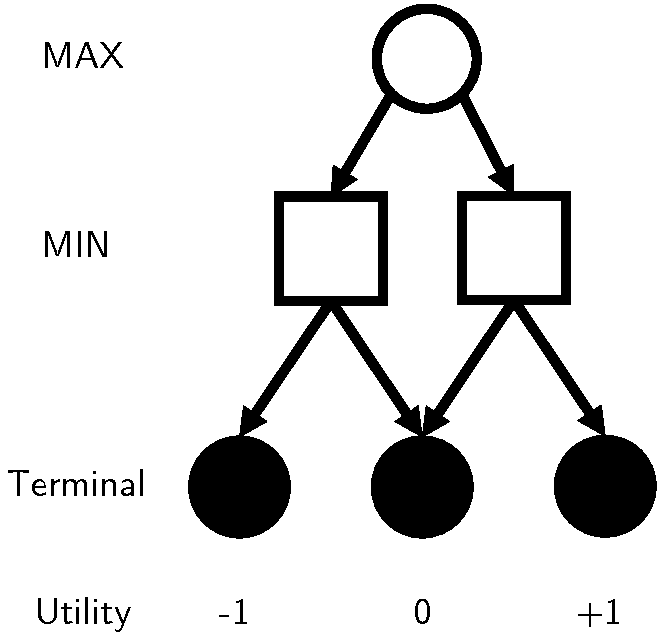
\includegraphics[scale=0.3]{minimax/minimax_step0.pdf}
      \caption{Spielbaum im Ausgangszustand}
      \label{fig:minimax_step0}
    \end{subfigure}
    \begin{subfigure}[b]{0.45\textwidth}
      \centering
      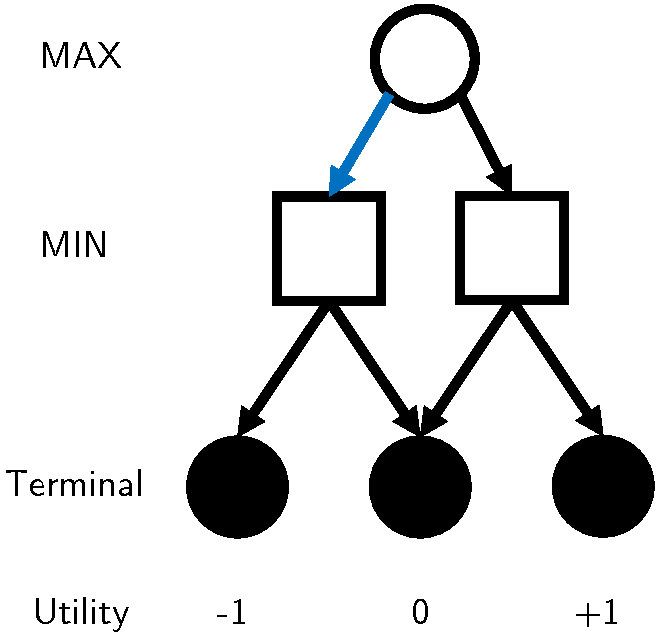
\includegraphics[scale=0.3]{minimax/minimax_step1.pdf}
      \caption{MAX prüft Utility der Kindknoten}
      \label{fig:minimax_step1}
    \end{subfigure}
    \begin{subfigure}[b]{0.45\textwidth}
      \centering
      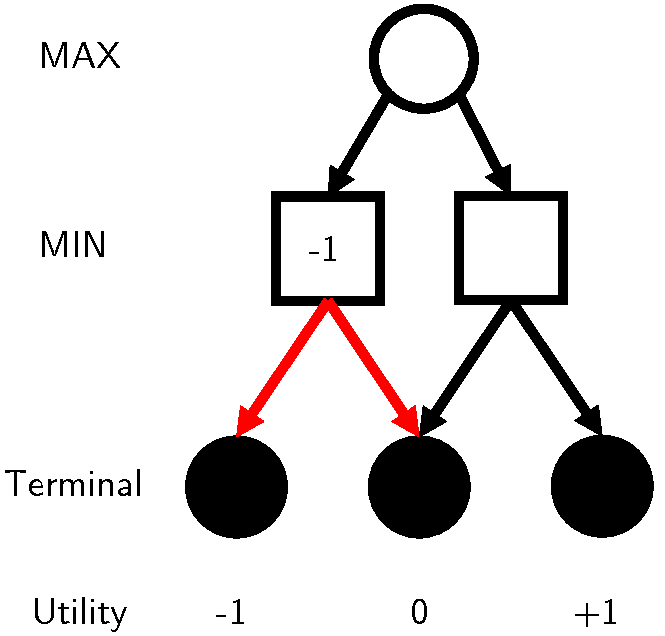
\includegraphics[scale=0.3]{minimax/minimax_step2.pdf}
      \caption{MIN prüft Utility der Terminalknoten und übernimmt kleinste Utility}
      \label{fig:minimax_step2}
    \end{subfigure}
    \begin{subfigure}[b]{0.45\textwidth}
      \centering
      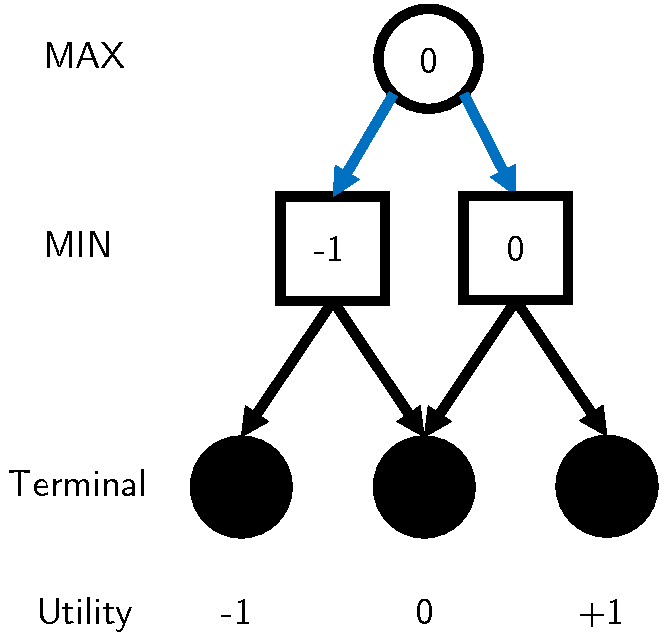
\includegraphics[scale=0.3]{minimax/minimax_step3.pdf}
      \caption{b) und c) werden für rechte Seite wiederholt und MAX wählt größte Utility aus}
      \label{fig:minimax_step3}
    \end{subfigure}
    \caption[Visualisierung des Minimax-Algorithmus]{Visualisierung des Minimax-Algorithmus für ein fiktives Zweispieler-Nullsummenspiel in vier Schritten. Knoten des maximierenden Spielers (MAX) sind Kreise, Knoten des minimierenden Spielers (MIN) Quadrate.}
    \label{fig:minimax_example}
\end{figure}

{\centering
\begin{minipage}{0.60\textwidth}
\begin{algorithm}[H]
\SetAlgoLined
\DontPrintSemicolon
\SetKwFunction{KwMinimax}{Minimax}
\SetKwProg{Fn}{Function}{:}{}
\Fn{\KwMinimax{NODE, PLAYER}}{
    \uIf{NODE is terminal}{
        \KwRet{utility assigned to NODE}
    }
    \uElseIf{PLAYER is maximizing player MAX}{
        \ForEach{child of NODE}{
            \KwMinimax{CHILD, MIN}\;
        }
        \KwRet{maximal CHILD utility}
    }
    \Else{
        \ForEach{child of NODE}{
            \KwMinimax{CHILD, MAX}\;
        }
        \KwRet{minimal CHILD utility}
    }
}
\textbf{end function}

\caption{Pseudocode Minimax-Algorithmus}
\label{algo_minimax}
\end{algorithm}
\end{minipage}
\par
}


Da manche Knoten in Spielbäumen durch unterschiedliche Zugfolgen erreicht werden können, kann der Minimax-Algorithmus durch eine Transposition table (\dt Zugumstellungs-Tabelle) erweitert werden.
Bei diesen werden Informationen zu Knoten in einer Lookup-Tabelle hinterlegt, sodass direkt auf diese zugegriffen werden kann. \cite[S. 651]{millingtonArtificialIntelligenceGames2009}, \cite[S. 22]{slateCHESSNorthwesternUniversity1983}, \cite[S. 807]{greenblattGreenblattChessProgram1988}
Der Name Transposition table leitet sich vom Schach ab, bei dem unterschiedliche Spielzüge, um einen gleichen Zustand zu erreichen, als Transposition (dt. Zugumstellung) bezeichnet werden \cite[S. 651]{millingtonArtificialIntelligenceGames2009}. 
Andere Vereinfachungen und Erweiterungen des Minimax-Algorithmus, wie beispielsweise \gqq{Negamax} oder Alpha-Beta-Pruning \cite[S. 115]{ertelIntroductionArtificialIntelligence2017} werden in dieser Arbeit nicht betrachtet.


\section{Tic-Tac-Toe}

In diesem Abschnitt wird das Strategiespiel Tic-Tac-Toe (\ac{TTT}) erklärt. Anschließend wird begründet, wieso die vorgestellten Algorithmen darauf angewandt werden können. 

\subsection{Spielerklärung}
\acl{TTT} ist ein Strategiespiel, das von zwei Spielern gespielt wird \cite[S. 6]{allisSearchingSolutionsGames1994}.
Das Spielfeld ist unterteilt in neun Bereiche (Slots), die in einer 3x3 Matrix angeordnet sind. 
%Die Slots gehören daher zu einer von drei Klassen, die als Ecken, Kanten oder Mitte bezeichnet werden. Zu Beginn sind alle Slots leer. 
Die Spieler platzieren abwechselnd ihr zugeteiltes Symbol, entweder X oder O, in einem Slot auf dem Spielfeld. 
Der beginnende Spieler verwendet in der Regel das Symbol X. 
Ziel jedes Spielers ist es, drei eigene Symbol entweder vertikal, horizontal oder diagonal in einer Reihe zu platzieren.
Somit gibt es insgesamt acht mögliche Gewinnkonstellationen: drei Zeilen, drei Spalten und zwei Diagonalen. 
Sind alle Slots belegt ohne, dass einer der Spieler gewonnen hat, endet das Spiel in einem Unentschieden. \cite[S. 533]{crowleyFlexibleStrategyUse1993}

\acs{TTT} besitzt 5478 legale Spielfeldkonstellationen und hat im Vergleich zu Spielen wie Schach oder Vier Gewinnt eine deutlich geringere Zustandsraum-Komplexität  \cite[S. 159]{allisSearchingSolutionsGames1994}.
Dies kann sogar weiter reduziert werden, da aufgrund von Rotations- und Spiegelsymmetrien bis zu acht Spielfeldkonstellationen äquivalent sein können.\footnote{4 Rotationen und 4 Spiegelungen, jeweils horizontal/vertikal mit und ohne 90° Drehung} 
Dadurch reduziert sich die Zustandsraum-Komplexität auf 765. \cite[S. 3]{block-berlitzm.ProInformatikFunktionaleProgrammierung2009}

In der Spieltheorie ist \acs{TTT} ein klassisches Beispiel für ein Nullsummenspiel, da ein Gewinn immer mit einer Niederlage für den Gegner einhergeht \cite[S. 6]{allisSearchingSolutionsGames1994}, \cite[S. 533]{crowleyFlexibleStrategyUse1993}.
Zudem gehört TTT zu den Spielen mit perfekter Information, weil beide Spieler Zugriff auf alle Informationen des aktuellen Spielzustands haben \cite[S. 156]{allisSearchingSolutionsGames1994}, \cite[S. 38]{gardnerm.HexaflexagonsOtherMathematical1988}.
\acs{TTT} ist ein stark gelöstes Spiel, \dahe es gibt eine optimale Strategie für jede legale Position \cite[S. 6]{allisSearchingSolutionsGames1994}
Spielen beide Spieler optimal endet TTT immer in einem Unentschieden und wird daher als futile Game (\dt vergebliches Spiel) bezeichnet \cite[S. 177]{wangPopularLecturesMathematical2014}.
Somit ist das beste Spielergebnis immer zu Gewinnen und gegen einen optimalen Spieler Unentschieden zu spielen. 
Regeln für ein perfektes Spiel wurden erstmals 1972 in \cite{newellHumanProblemSolving1972} formuliert. 
\citeauthor{crowleyFlexibleStrategyUse1993} erweiterten diese unter der Bezeichnung \gqq{Model of Expert Performance}, wie im Anhang \cref{chap:ModelofExpert} gelistet \cite[S. 536]{crowleyFlexibleStrategyUse1993}. 
Die folgenden vier Regeln \bzw Aktionen bilden in der dargestellten Reihenfolge die zentrale Strategie für Expert Play. Beispielhafte Spielfeldkonstellationen werden in Abbildung \cref{fig:ttt_expertplay} gezeigt.

\begin{enumerate}
    \item \textbf{Win}: Wenn der Spieler eine Möglichkeit hat zu gewinnen, soll diese genutzt werden
    \item \textbf{Block}: Wenn der Gegner zwei Symbole in einer Reihe hat, blockiere den Gewinn des Gegners
    \item \textbf{Fork}: Wenn sich zwei Reihen schneiden, in denen der Spieler sein Symbol platziert hat und der Slot, wo sie sich schneiden leer ist, belege diesen Slot
    \item \textbf{Block Fork}: Wenn die Möglichkeit besteht, zwei Symbole in eine Reihe zu legen, wähle diesen Slot, um den Gegner zum Blocken zu zwingen. Andernfalls wähle einen Slot, um ein Fork des Gegners zu verhindern
\end{enumerate}

\begin{figure}
    \centering
    \begin{subfigure}[b]{0.45\textwidth}
      \centering
      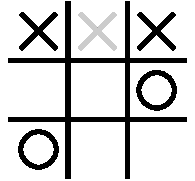
\includegraphics[scale=0.7]{ttt_boards/ttt_win.pdf}
      \caption{Win}
      \label{fig:ttt_win}
    \end{subfigure}
    \begin{subfigure}[b]{0.45\textwidth}
      \centering
      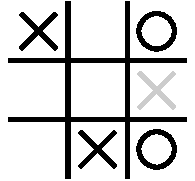
\includegraphics[scale=0.7]{ttt_boards/ttt_block.pdf}
      \caption{Block}
      \label{fig:ttt_block}
    \end{subfigure}
    \begin{subfigure}[b]{0.45\textwidth}
      \centering
      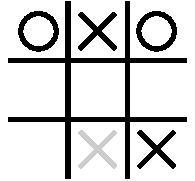
\includegraphics[scale=0.7]{ttt_boards/ttt_fork.pdf}
      \caption{Fork}
      \label{fig:ttt_fork}
    \end{subfigure}
    \begin{subfigure}[b]{0.45\textwidth}
      \centering
      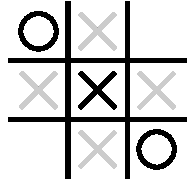
\includegraphics[scale=0.7]{ttt_boards/ttt_blockfork.pdf}
      \caption{Block Fork}
      \label{fig:ttt_blockfork}
    \end{subfigure}
    \caption[Beispielhafte Spielfeldkonstellationen für TTT Expert Play]{Beispielhafte Spielfeldkonstellationen für \acs{TTT} Expert Play. Optimale Aktionen sind grau gefärbt \protect\footnotemark}
    \label{fig:ttt_expertplay}
\end{figure}

\footnotetext{Spielfeldkonstellationen übernommen aus \cite[S. 539]{crowleyFlexibleStrategyUse1993}, Alle \acs{TTT} Spielfelder werden erstellt mit Code von \cite{sebglavCreatingTicTacToeBoards2022}}

Der zweite Teil der Strategie beschäftigt sich mit dem optimalen ersten Zug für X. 
Aufgrund der Äquivalenz der möglichen Aktionen reduziert sich die Auswahl auf drei Möglichkeiten: Ecke, Kante und Mitte. 
In \cite[S. 38]{gardnerm.HexaflexagonsOtherMathematical1988} wird die Ecke als stärkste Aktion dargestellt, da der Gegner mit der Mitte kontern muss, um nicht zu verlieren. 
Hingegen zeigen Studien wie \cite{kutscheraa.BestOpeningMove2018}, dass die Mitte die beste Aktion ist, da diese in der Menge aller möglichen Spielabfolgen die Startposition mit den meisten gewonnen Spielen ist.
Spielen zwei optimale Spieler gegeneinander ist die Wahl der ersten Aktion unbedeutend \cite[S. 38]{gardnerm.HexaflexagonsOtherMathematical1988}.

\subsection{Anwendbare Algorithmen}
\label{sec:anwendbare_algorithmen}
Eine Voraussetzung für die Anwendung des Minimax-Algorithmus ist, dass der Spielbaum eine geringe Komplexität hat \cite[S. 10]{block-berlitzm.ProInformatikFunktionaleProgrammierung2009}.
Die Spielbaum-Komplexität ist definiert als die Anzahl der Terminalknoten des vollständig konstruierten Spielbaums und wird angegeben als $\log$ zur Basis $10$ \cite[S. 160]{allisSearchingSolutionsGames1994}.
Aufgrund des kleinen Zustands- und Aktionsraums von \ac{TTT}, ist dessen Spielbaum klein.
Die Spielbaum-Komplexität beträgt $5$ ist im Vergleich zu Spielen wie Schach (123) oder Shogi (226) relativ gering \cite[S. 11]{block-berlitzm.ProInformatikFunktionaleProgrammierung2009}.
Somit erfüllt \ac{TTT} diese Bedingung für die Anwendung des Minimax-Algorithmus.
Eine weitere Bedingung des Minimax-Algorithmus ist, dass das Spiel ein Zweispieler-Nullsummenspiel mit perfekter Information sein muss \cite[S. 10]{block-berlitzm.ProInformatikFunktionaleProgrammierung2009}. 
Da \ac{TTT} auch diese Bedingung erfüllt, kann der Minimax-Algorithmus angewendet werden.
In \cref{fig:ttt_tree} ist ein Auszug des Spielbaums von \acs{TTT} mit der möglichen Umsetzung eines Minimax-Algorithmus dargestellt. Jedoch ist anzumerken, dass der Minimax-Algorithmus einen optimalen Gegner erwartet und daher nur gegen diese optimal spielt. Minimax kann nicht verlieren, aber wählt seine Aktionen nicht, um seine Gewinnwahrscheinlichkeit gegen nicht optimale Spieler zu maximieren. \cite[S. 8]{suttonLearningPredictMethods1988}. 

Voraussetzung für die Anwendung von \ac{TDL} Algorithmen ist, dass das zu lösende Problem als \ac{MDP} formuliert werden kann.
Der mögliche Zustandsraum $S$ und Aktionsraum $A$ sind für \ac{TTT} diskret und bekannt. 
Da \ac{TTT} ein Spiel mit perfekter Information ist, kann bei gegebenem Zustand $s$ und Aktion $a$ der Folgezustand $s'$ bestimmt werden.
Somit erfüllt \ac{TTT} die Markov Eigenschaft und kann als ein \ac{MDP} modelliert werden.
Die weitere Voraussetzung ist, dass der Agent mit seiner Umgebung interagieren kann und von dieser Samples in Form des Tupels $(S_t,A_t,R_{t+1},S_{t+1})$ erhält. \cite[S. 88]{kontesg.SeminarReinforcementLearning2021}
Diese kann im Rahmen der Implementierung beachtet werden. 
Da somit beide Voraussetzungen erfüllt sind, können \ac{TDL} Methoden wie \bothAlgs angewendet werden.

\begin{figure}[h]
    \centering
    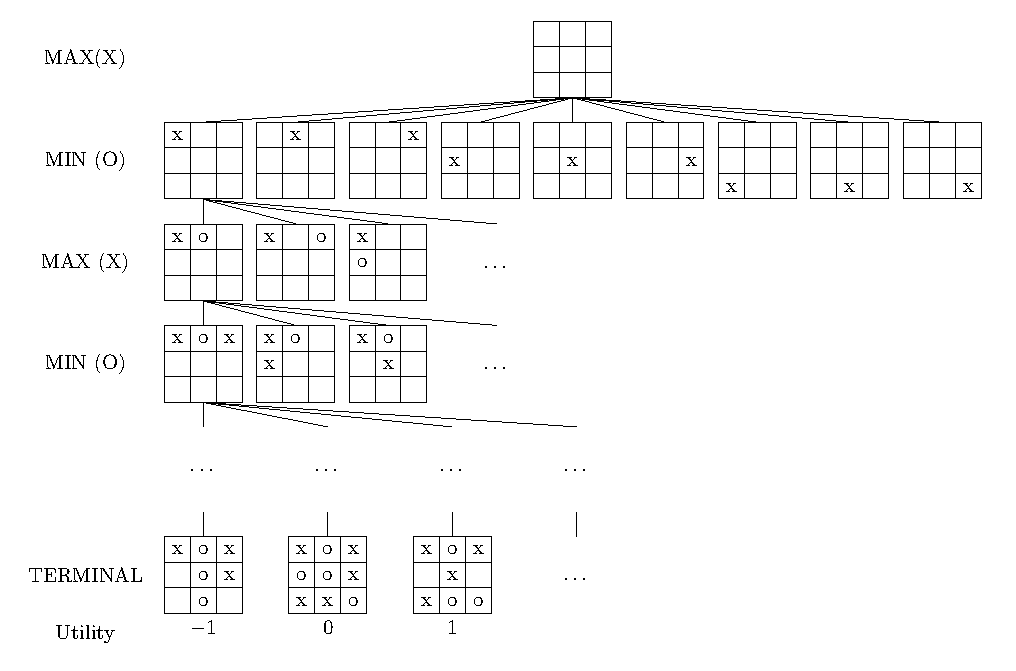
\includegraphics[scale=0.7]{04_Artefakte/01_Abbildungen/ttt_boards/ttt_tree.pdf}
    \caption[Auszug aus dem Spielbaum von \acs{TTT}]{Auszug aus dem Spielbaum von \acs{TTT} \protect\footnotemark}
    \label{fig:ttt_tree}
\end{figure}

\footnotetext{Darstellung übernommen aus \cite[S. 125]{russellArtificialIntelligenceModern2021}, Abbildung erstellt mit Code von \cite{vj.l.TikzPgfFollowup}}

\chapter{Methodik und Anwendung der Algorithmen}
In diesem Kapitel wird erklärt, wie die vorgestellten \ac{TD} Konzepte auf \ac{TTT} angewandt werden können.
Anschließend wird beschrieben, wie \ac{TTT} als Umgebung genutzt wird.
Abschließend wird die Vorgehensweise beim Training und der Evaluation vorgestellt.
\section{Anwendung von Temporal-Difference Learning auf \ttt}
\label{sec:TDL_TTT}
Die folgenden Abschnitte behandeln die Umsetzung des Temporal-Difference Update und einer möglichen Rewardfunktion. 
Anschließend wird der Aufbau der Q-Tabelle erklärt und das Konzept der Afterstates eingeführt.

\subsection{Temporal-Difference Update und Rewardfunktion}

Zur Anwendung von \acl{RL} muss definiert werden, was die Bestandteile des \ac{MDP} sind. 
In \acl{TTT} entspricht das Spielfeld der Umgebung und ein Zustand $s$ ist eine Konstellation des Spielfeldes. 
Der Agent ist ein Spieler, der als Aktion einen freien Slot wählt, in dem das zugewiesene Symbol platziert wird. 
Die Menge der legalen Aktionen in einem Zustand $A(s)$ entspricht den unbelegten Slots auf dem Spielfeld. 
Ein Spiel kann aus maximal neun Zeitschritten bestehen und endet immer mit einem Ergebnis. 
\acs{TTT} gehört daher zu den episodischen \ac{RL} Problemen.

Die Abweichung von klassischen \ac{RL} Problemen ist, dass zwei Agenten abwechselnd Symbole platzieren. Da das klassische \ac{TDL} nicht für Multi-Agenten Probleme definiert ist, kann es nicht direkt angewendet werden \cite[S. 2f. ]{vanderreeReinforcementLearningGame2013}. 
Eine mögliche Lösung bietet die Agenten-Umgebung-Schnittstelle. 
Demnach kann der Gegner und dessen gewählte Aktionen als Teil der Umgebung betrachtet werden, da der Agent diesen nicht kontrolliert. 
Somit erhält der Agent von der Umgebung nur die Zustände, in denen er eine Aktion wählen kann.
Aus Sicht des Agenten ist \acs{TTT} eine stochastische Umgebung, da der Zug des Gegners und somit der nächste Zustand, den ein Agent erhält nicht deterministisch sind. \cite[S. 2f]{vanderreeReinforcementLearningGame2013}, \cite{soemersd.GameAiHow} 
Unter der Voraussetzung, dass X beginnt, können alle Zustände gerader Zeitschritte \bzw Symbolanzahl dem Agenten X und ungerade dem Agent O zugeordnet werden, wie in Abbildung \cref{fig:ttt_state_to_agent} dargestellt.
Die zugehörigen \ac{MDP} beziehen sich nun auf einen Agenten, sodass die vorgestellten Algorithmen angewendet werden können.

\begin{figure}
    \centering
    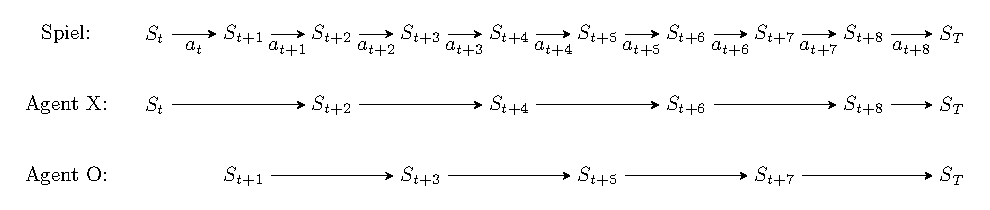
\includegraphics[width=\linewidth]{04_Artefakte/01_Abbildungen/ttt_state_to_agent.pdf}
    \caption{Zuordnung der \acs{TTT} Zustände und Zeitschritte zu den Agenten }
    \label{fig:ttt_state_to_agent}
\end{figure}

Für das \ac{TD} Update ist neben dem jetzigen Zustand $S_t$und der gewählten Aktion $a_t$ der nächste Zustand $S_{t+2}$, den der Agent erhält, notwendig. 
Da der nächste Zustand des Agenten abhängig von der Aktion des Gegners ist, erfolgt ein Update für einen Zustand erst, wenn der Gegner eine Aktion durchgeführt hat. 
Eine Besonderheit sind Terminalzustände, da diese das Spiel beenden und somit keine Aktion durch den Gegner möglich ist. 
Ein Terminalzustand $S_T$ wird erreicht, wenn ein Spieler eine Aktion wählt, durch die er das Spiel gewinnt oder in einem Unentschieden beendet. 
Wechselt ein Agent durch eine Aktion in einen Terminalzustand, wird dieser für das Update beider Agenten verwendet. \cite[S. 2f]{vanderreeReinforcementLearningGame2013}, \cite{soemersd.GameAiHow}
Dies ist möglich, da der \qValue jedes Terminalzustands per Definition 0 ist \cite[S. 74]{suttonReinforcementLearningIntroduction2018}. 
Die Unterscheidung, ob ein Spielergebnis gut oder schlecht für den Agenten ist, erfolgt im Update durch den Reward.

Beim Minimax-Algorithmus erhalten beide Symbole die gleiche Utility, weshalb es einen minimierenden und maximierenden Spieler gibt.
Die \ac{TD} Agenten hingegen versuchen ihren Return zu maximieren, sodass Reward positiv oder negativ, entsprechend des Spielergebnisses aus Agenten-Sicht sein muss.
\acs{TTT} ist ein Nullsummenspiel mit drei möglichen Spielergebnissen: Gewinn, Niederlage und Unentschieden.
Wie in \cref{sec:minimax} beschrieben, ist eine gängige Zuordnung $+1$, $-1$ und $0$.
Das Spielverhalten kann jedoch weiter differenziert werden durch Betrachtung der Spiellänge, gemessen in durchgeführten Aktionen. 
Ein optimaler Agent sollte versuchen, in möglichst wenigen Zügen zu gewinnen und eine Niederlage möglichst lange hinauszögern \cite[S. 533]{crowleyFlexibleStrategyUse1993}. 
Eine mögliche Umsetzung ist, den Reward je Spielzug in der Episode um $0.1$ gegen $0$ zu korrigieren.
Als Korrektur wird $0.1$ verwendet, da neun Spielzüge möglich sind und selbst bei Gewinn im letzten Zug ein positiver Reward zugewiesen wird.
Diese Korrektur wird im Folgenden als \gqq{Depth Penalty} bezeichnet, da eine Korrektur entsprechend der Tiefe (\engl depth) im Spielbaum erfolgt.
Dieser Reward bewertet, ob der Agent das Ziel, \acs{TTT} zu Gewinnen, erreicht hat und wird daher als letzter Reward einer Episode ausgeteilt.
Die Rewards aller anderen Aktionen sind 0, da deren Bedeutung für das Spielergebnis nicht bekannt ist. 
Der Reward kann somit mittels \cref{eq:depth_penalty} berechnet werden und  liefert die in \cref{tab:reward_depth_penalty} gelisteten Rewards.
Da der unkorrigierte Reward für Sieg und Niederlage $1$ und $-1$ ist, kann er genutzt werden, um das Vorzeichen der Korrektur anzupassen.
Andere Definitionen eines Rewards sind möglich, werden in dieser Arbeit jedoch nicht betrachtet \cite{mirnovi.QLearningTicTacToe2020}.

\begin{equation}\label{eq:depth_penalty}\equationentry{Formel für korrigierten Reward mit Depth Penalty}
   \text{reward}_{\text{angepasst}}= \text{reward}- (\text{reward}\cdot \text{depth} \cdot 0,1)
\end{equation}

\begin{table}
\centering
\caption{Mögliche Rewards pro Spielzug bei Korrektur des Rewards mittels Depth Penalty}
\label{tab:reward_depth_penalty}
\begin{tabular}{lrr}
\toprule
 Zug   & Reward Agent  & Reward Gegner \\ \midrule
1      & /              & / \\
2      & /              & / \\
3      & /              & / \\
4      & /              & / \\
5      & 0,5            & -0,5\\
6      & -0,4           & 0,4 \\
7      & 0,3            & -0,3\\
8      & -0,2           & 0,2 \\
9      & 0,1            & -0,1 \\ \bottomrule
\end{tabular}
\end{table}


\subsection{\qtable und Kompression durch Afterstates}
\label{sec:afterstates}

Die \qtable enthält die Abbildung der \ac{SA Tupel} auf einen \qValue. 
Da jeder Zustand und somit jedes \ac{SA Tupel} eindeutig einem Symbol zugeordnet werden kann, können die \qValues für beide Symbole in einer gemeinsamen \qtable gespeichert werden. 
Wird die \qtable als eine Lookup-Tabelle visualisiert, wie in \cref{tab:qtable_example}, enthält diese für jeden der 5478 Zustände eine Zeile. 
Die Aktionen sind die Spalten, wobei die Aktionen nicht für jeden Zustand gleich sind, sondern den freien Slots auf dem Spielfeld entsprechen.

\begin{table}
\centering
\caption[Q-Tabelle für \acs{TTT}]{\qtable für \acs{TTT}. $S_{5477}$ ist ein Beispiel für einen Terminalzustand, in dem keine Aktionen möglich sind, dargestellt durch \gqq{/}}
\label{tab:qtable_example}
\begin{tabular}{lllll}
\toprule
State       &   $a_0$           &   $a_1$       & $\dots$   & $a_8$         \\ \midrule
$S_0$       &   $Q(S_0,a_0)$    &  $Q(S_0,a_1)$ & $\dots$   & $Q(S_0,a_8)$  \\
$S_1$       &   $Q(S_1,a_0)$    &  $Q(S_1,a_1)$ & $\dots$   & $Q(S_1,a_8)$  \\
$\vdots$    & $\vdots$          & $\vdots$      & $\ddots$  & $\vdots$      \\
$S_ {5477}$    &  /                 &  /           & $\dots$   & /  \\ \bottomrule
\end{tabular}
\end{table}


Wie im vorigen Abschnitt  beschrieben, besteht eine Runde aus einem deterministischen Zustandswechsel durch den Agenten und einem stochastischen Zustandswechsel durch die Umgebung.
In \acs{TTT} können unterschiedliche \ac{SA Tupel} dieselbe Spielfeldkonstellation erzeugen, bevor der Gegner zum Zug kommt, wie in \cref{fig:ttt_afterstate} dargestellt. 
Die Zustände nach dem deterministischen Zustandswechsel durch den Agenten werden als Afterstate (\dt Folgezustand) bezeichnet und können als surjektive Abbildung der \ac{SA Tupel} auf die Menge der Afterstates $Y$ beschrieben werden: $(S,A) \rightarrow Y$.  
\ac{SA Tupel}, die denselben Afterstate haben, sollten einen gemeinsamen \qValue besitzen. 
Dadurch wird Erfahrung, die durch ein \ac{SA Tupel} gesammelt wird, mit den anderen geteilt, sodass der Lernprozess beschleunigt wird. \cite[S. 136f.]{suttonReinforcementLearningIntroduction2018}

\begin{figure}
    \centering
    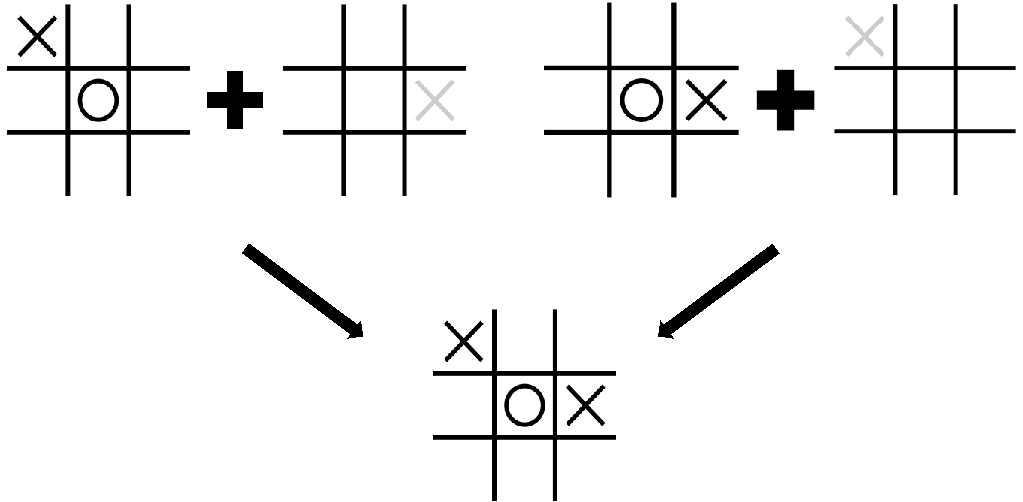
\includegraphics[scale=0.4]{04_Artefakte/01_Abbildungen/ttt_boards/ttt_afterstate.pdf}
    \caption[Beispiel für Afterstates in \acs{TTT}]{Beispiel für Afterstates in \acs{TTT}. Zwei \ac{SA Tupel} können im selben Afterstate resultieren \protect\footnotemark}
    \label{fig:ttt_afterstate}
\end{figure}

\footnotetext{Abbildung entnommen aus \cite[S. 137]{suttonReinforcementLearningIntroduction2018}}
Mit der vorgestellten \qtable ist dies jedoch nicht möglich, da die \qFunction jedem \ac{SA Tupel} einen individuellen \qValue zuweist und der resultierende Zustand dem anderen Symbol zugeordnet ist. 
Daher wird eine \afterStateVFunction genutzt, die statt einem \ac{SA Tupel} $(S,A)$ dem resultierenden Afterstate $y$ einen Wert zuweist. 
Der zugewiesene Wert kann, zur Unterscheidung vom \qValue, als \wValue $w$ bezeichnet werden.\cite{nbroReinforcementLearningHow}

Ein Agent wählt nun in einem Zustand, die Aktion, die im Afterstate mit dem höchsten \wValue resultiert. 
Die bisherige \qtable wird geteilt in zwei separate Tabellen, wie in  \cref{tab:afterstate} und \cref{tab:wtable} dargestellt. 
Einerseits die surjektive Abbildung $(S,A) \rightarrow Y$ sowie die Zuweisung des \wValue zu einem Afterstate: $y \rightarrow w$, die im Folgenden als \afterstateTable und \wtable bezeichnet werden. 
Im Gegensatz zur \qtable umfasst der \wtable nur 5477 Zeilen, da der Ausgangszustand kein Afterstate ist. 
Die Anzahl der \wValues ist im Vergleich zur Anzahl von \qValues deutlich komprimiert, da \ac{SA Tupel}, die denselben Afterstate $y$ haben einen \wValue teilen.
Streng genommen benötigt ein Agent mit \afterStateVFunction nur die Menge der erreichbaren Afterstates und nicht den Zustand oder die legalen Aktionen selbst, da diese durch die Abbildung $(S,A) \rightarrow Y$ implizit enthalten sind. \cite{nbroReinforcementLearningHow}

\begin{table}[!htb]
    \begin{minipage}{.5\textwidth}
        \centering
        \caption{\afterstateTable für \acs{TTT}}
        \label{tab:afterstate}
        \begin{tabular}{lllll}
        \toprule
        State       & $a_0$     & $a_1$     & $\dots$     & $a_8$   \\ \midrule
        $S_0$       & $y_0$     & $y_1$     & $\dots$     & $y_8$   \\
        $S_1$       & $y_1$     & $y_0$     & $\dots$     & $\dots$ \\
        $\vdots$    & $\vdots$  & $\vdots$  & $\ddots$    & $\vdots$ \\
        $S_{5477}$  & $\dots$   & $\dots$   & $\dots$    &  $\dots$\\ \bottomrule
        \end{tabular}
    \end{minipage}%
    \begin{minipage}{.5\textwidth}
        \centering
        \caption{\wtable für \acs{TTT}}
        \label{tab:wtable}
        \begin{tabular}{ll}
        \toprule
        Afterstate  & \wValue       \\ \midrule
        $y_0$       & $w(y_o)$      \\
        $y_1$       & $w(y_1)$      \\
        $\vdots$    & $\vdots$      \\
        $y_{5476}$  & $w(y_{5476})$ \\ \bottomrule
        \end{tabular}
    \end{minipage}
\end{table}


\section{Kodierung von \ttt}
\label{chap:ttt_encoding}

Das \acl{TTT} Spielfeld besteht aus neun Slots, die entweder leer oder durch ein Symbol belegt sind.  
Ein Spielfeld kann daher als Folge von Bits betrachtet werden. 
Diese Form der Kodierung wird als Bitboard bezeichnet und genutzt zur speichereffizienten Beschreibung von Spielfeldern, die mit Bitoperationen manipuliert werden können. \cite[S. 86]{slateCHESSNorthwesternUniversity1983}

Werden die Slots, beginnend bei $0$, von oben links nach unten rechts indexiert, kann der Zustand eines Spielfeldes als neunstellige Binärzahl $B_G$ ausgedrückt werden. 
Der Index eines Slots ist der Exponent zur Basis 2. 
Beispielsweise beschreibt der Zustand $0_2$ ein leeres Spielfeld und $111000000_2$ die Konstellation, in der die Slots $0-5$ frei sind und die letzte Reihe gefüllt ist, wie in \cref{fig:ttt_index_and_bottomrow} dargestellt.

\begin{figure}
    \centering
    \begin{subfigure}[b]{0.45\textwidth}
      \centering
      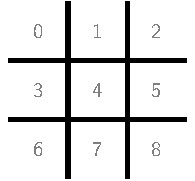
\includegraphics[scale=0.7]{ttt_boards/ttt_index.pdf}
      \caption{Indexierung der Slots}
      \label{fig:ttt_index}
    \end{subfigure}
    \begin{subfigure}[b]{0.45\textwidth}
      \centering
      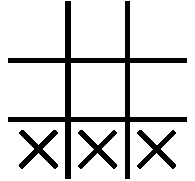
\includegraphics[scale=0.7]{ttt_boards/ttt_bottom_row_x.pdf}
      \caption{Zustand $111000000_2$}
      \label{fig:ttt_bottom_row_x}
    \end{subfigure}
    \caption{\acs{TTT} Indexierung und Beispiel für $B_G$}
    \label{fig:ttt_index_and_bottomrow}
\end{figure}

Jedoch sind neun Bits nicht ausreichend, da zwischen zwei verschiedenen Symbolen und somit insgesamt drei Zuständen pro Slot unterschieden werden muss. 
Daher muss die Konstellation des Spielfeldes für jedes Symbol in einem dedizierten Bitboard kodiert werden, die im Folgenden als $B_X$ und $B_O$ bezeichnet werden.

Durch Konkatenation der beiden Bitboards \bzw Binärzahlen ist die Kodierung des gesamten Spielfeldes mit Unterscheidung der Symbole  für einen Zustand $s$ in einer 18-stelligen Binärzahl möglich. 
Diese wird als $B_{s}$ bezeichnet. 
Dabei wird festgelegt, dass die ersten neun Bits für $B_O$ und die anderen für $B_X$ stehen. Der Wert von $B_s$ zur Basis $10$ kann mit \cref{eq:bitboard_bs} eineindeutig berechnet werden. 


\begin{equation}\label{eq:bitboard_bs}\equationentry{Berechnung des Zustandsidentifikators $B_s$}
   B_s= \sum_{i=9}^{17}2^{i}\cdot \mathbbm{1}_{X_i=true} + \sum_{i=0}^{8}2^{i}\cdot \mathbbm{1}_{O_i=true}
\end{equation}

Durch Logische OR Verknüpfung der Bitboards beider Symbole kann die neunstellige Spielfeldkodierung $B_G$ vom Anfang erreicht werden, die nicht zwischen Symbolen unterscheidet: $B_X \lor B_O = B_G$. 
Die Bits in $B_G$ mit Wert False sind die freien Slots und kodieren die Menge der legalen Aktionen $A$. 
Somit hat ein Agent maximal neun mögliche Aktionen, die im Interval $[0; 8]$ liegen. 
Wird eine Aktion von einem Spieler durchgeführt, so wird der Index des von ihm belegten Slot in seinem eigenen Bitboard auf True gesetzt.
Ein Beispiel für eine Kodierung einer Spielfeldkonstellation ist in \cref{fig:ttt_163968} dargestellt.

\begin{figure}
   \begin{minipage}[c]{.5\textwidth}
   \centering
    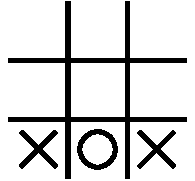
\includegraphics[scale=0.7]{04_Artefakte/01_Abbildungen/ttt_boards/ttt_163968.pdf}
   \end{minipage}%
   \begin{minipage}[c]{.5\textwidth}
      $B_G = 111000000_2$ \\
      $B_X = 101000000_2$ \\
      $B_O = 010000000_2$ \\
      $B_s = 101000000010000000_2 = 163968_{10}$
   \end{minipage}
   \caption{Beispiel für die unterschiedlichen Spielfeldkodierungen}
   \label{fig:ttt_163968}
\end{figure}

Die acht möglichen Gewinnkonstellationen $M_{i} \mid i \in [1,8]$ von \acs{TTT} können durch Bitoperationen geprüft werden.
Dafür wird eine logische AND Operation einer der Gewinnkonstellationen mit dem Bitboard eines Spielers durchgeführt und das Ergebnis auf Äquivalenz mit der ursprünglichen Gewinnkonstellation geprüft: $B_X \land M_i = M_i$. 
Ist die Äquivalenz dieser Gleichung gegeben, bedeutet dies, dass die Gewinnkonstellation $M_i$ vorliegt

Da ein Spieler nur Aktionen durchführen kann, die eine Gewinnkonstellation für ihn selbst konstruieren, muss nach einer Aktion nur das Bitboard des Spielers geprüft werden, der die letzte Aktion durchgeführt hat. 
Liegt keine Gewinnkonstellation vor und das Bitboard $B_G$ enthält keine Bits mit Wert False, endet das Spiel in einem Unentschieden.
\section{Trainingsaufbau der Agenten}
In den folgenden Abschnitten wird der verwendete Trainingsaufbau erklärt. 
Dies umfasst die Arten von \splay sowie die Auswahl der Hyperparameter, die untersucht werden.
Abschließend werden die genutzten Metriken vorgestellt.

\subsection{\splay}
Zum Training spielt ein Agent wiederholt gegen Gegner. 
Die Spielstärke der Gegner sollte vergleichbar mit der des Agenten sein und während des Trainings steigen \cite[S.1 ff.]{epsteinIdealTrainer1994}.
Da die Bereitstellung unterschiedlicher Gegner ansteigender Spielstärke für komplexere Strategiespiele nicht praktikabel ist, gibt es das Konzept des \splay. \cite[S. 565f.]{szitaReinforcementLearningGames2012} \cite[S. 1ff.]{digiovanniSurveySelfPlayReinforcement2021}
Im \splay lernt der  Agent das Spiel, indem er gegen eine Kopie von sich selbst spielt. 
Dadurch wird stetig gegen einen Gegner gleicher Stärke gespielt, ohne dass dieser zusätzlich implementiert werden muss \cite[S. 565f.]{szitaReinforcementLearningGames2012}.
Jedoch hat \splay das Problem, das beide Agenten gleichzeitig lernen und in lokalen Maxima stecken bleiben können. 
Dies hat zur Folge, dass das Lernen unvollständig ist und die Agenten frühzeitig mit dem Lernen aufhören und den Zustandsraum nicht ausreichend erkunden. \cite[S. 16]{boyanModularNeuralNetworks1992}, \cite[S. 565f.]{szitaReinforcementLearningGames2012}, \cite{bowlingConvergenceNoRegretMultiagent2004}

Eine Möglichkeit den Zustandsraum repräsentativer zu proben, ist die Agenten abwechselnd lernen zu lassen. 
Während ein Agent lernt, nutzt der andere seine derzeitige  greedy Policy\footnote{Hyperparameter werden entsprechend gesetzt: $\alpha = \epsilon = 0$}.
Nach einer festen Anzahl von Episoden, die im Folgenden Batch genannt werden, wechseln die Rollen. \cite{slatern.GameAiWhy} 
Dies wird wiederholt, bis die Trainingsepisodenanzahl erreicht wurde, wie im Algorithmus \ref{algo_selfplay} dargestellt.
Da zu Beginn des Trainings der Agent das Spiel nicht kennt, spielt der lernende Agent im ersten Batch gegen einen Spieler mit Zufallsstrategie. 

Im Rahmen der Bachelorarbeit werden das klassische \splay und das beschriebene \splay mit alternierenden Rollen für \ttt implementiert und in der Auswertung verglichen. 
Aufgrund von Vorexperimenten wird festgelegt, dass in beiden Fällen zum Training 150.000 Episoden gespielt werden. Ein Batch beim alternierendem \splay umfasst 100 Episoden.

{\centering

\begin{minipage}{0.65\textwidth}

\begin{algorithm}[H]
\SetAlgoLined
\DontPrintSemicolon
\SetKwInput{Kwinput}{Input}

\Kwinput{$agentX$, $agentO$, $training\_episodes$}
$learningAgent \leftarrow agentX$ \;
set hyperparameters of both agents according to their role\;
\For{$episode \leftarrow 0$ \KwTo $training\_episodes$}{
    play an episode of tic-tac-toe\;
    \If{episode $\bmod$ batch$\_$size = 0}{
        switch learningAgent\;
        set hyperparameters of both agents according to their role\;
}

}
\caption{Pseudocode alternierendes \splay}
\label{algo_selfplay}
\end{algorithm}
\end{minipage}
\par
}

\subsection{Auswahl der Hyperparameter}
\label{sec:hyperparameter}
Die Hyperparameter können entweder konstant sein oder im Verlauf des Trainings abnehmen. 
Zur Komplexitätsreduktion wird für die Verkleinerung von Hyperparametern nur eine Methode genutzt.
Diese Methode zur degressiven Abnahme wird als Step-Based bezeichnet und ist durch folgende Formel für einen beispielhaften Parameter $\eta$ definiert \cite[S. 3]{parkNovelLearningRate2020} :

\begin{equation}\label{eq:Eq3}\equationentry{Step-Based Parameterabnahme}
   \eta(x) = \eta_{start}(\frac{\eta_{end}}{\eta_{start}})^{\frac{x}{x_{max}}}
\end{equation}

Der Parameter $\eta$  hat in der ersten Episode ($x=0$) den Wert $\eta_{start}$ und in der Episode $x_{max}$ den Wert $\eta_{end}$. 
Mit steigender Episode $x$ wird die Anpassung zunehmend kleiner. 
Zur weiteren Komplexitätsreduktion wird nur eine kleine Untermenge möglicher Parameterkombinationen untersucht, die durch Vorexperimente ausgewählt wurden. 

Als Diskontierungsfaktor $\gamma$ wird $1$ verwendet, da \acs{TTT} ein endliches Spiel und die Diskontierung somit nicht notwendig ist. 
Da die Definition des optimalen Verhaltens bereits durch den Reward erfolgt, wird $\gamma$ nicht weiter betrachtet.

Die Lernrate $\alpha$ muss während des Trainings gemindert werden, um die Konvergenz der Algorithmen zu gewährleisten. 
Jedoch wird diese Konvergenzbedingung nur selten in der Praxis eingehalten. 
Zudem ist in nicht-stationären Umgebungen eine konstante (kleine) Lernrate zu bevorzugen. \cite[S. 33]{suttonReinforcementLearningIntroduction2018} 
Da der Gegner vom Agent als Teil der Umgebung betrachtet wird und im klassischen \splay die Agenten gleichzeitig lernen, kann \acs{TTT} als nicht-stationäre Umgebung aufgefasst werden.  
In Vorexperimenten zeigte sich, dass konstante $\alpha$  genutzt werden können, wenn $\alpha < 0.3$ gilt.
Daher werden $\alpha=0,1$, $\alpha=0,2$ sowie ein $\alpha$, das zu Beginn $1$ ist und dann gegen $0.1$ konvergiert untersucht, 

Der Explorationswahrscheinlichkeit $\epsilon$ muss so gewählt werden, dass möglichst alle \ac{SA Tupel} besucht werden.
Insbesondere für \sarsa ist es jedoch notwendig, dass $\epsilon$ keinen konstant hohen Wert hat, damit Exploitation erfolgen kann. 
Durch Vorexperimente wurde ermittelt, dass dies zuverlässig erfolgt, wenn zu Beginn $\epsilon = 1$ gilt und im Rahmen des Trainings abnimmt und nach zwei Drittel der Episoden $\epsilon = 0.1$ gilt.
\section{Evaluation und Metriken}
\label{sec:eval_metrik}
Zur Beantwortung der Forschungsfragen werden die Algorithmen mit unterschiedlichen Hyperparameterkombinationen hinsichtlich ihrer Konvergenz und Spielstärke bewertet. Außerdem soll ermittelt werden, was laut den Agenten die optimale erste Aktion für das Symbol X ist.
Während der Trainings- und Evaluationsepsioden werden Daten gesammelt, auf Episoden-Ebene aggregiert und geloggt, sodass diese ausgewertet und geplottet werden können. 
Zum Plotten aller Liniendiagramme in dieser Arbeit wird die Python Bibliothek Matplotlib \cite{hunterMatplotlib2DGraphics2007} verwendet. 
Das dafür angefertigte Jupyter Notebook wird auf \href{http://github.com/JonasBingel/ThesisHSMZ-RLTicTacToe-Jupyter}{Github.com/JonasBingel} bereitgestellt.

Ein interessanter Aspekt beim Vergleich von RL-Algorithmen ist, wie schnell diese während des Trainings zur optimalen Policy konvergieren \cite[S. 33]{suttonReinforcementLearningIntroduction2018}. 
Als Konvergenzmetrik wird die Rate optimaler Aktionen, die vom Agent gewählt werden, genutzt.
Mit zunehmendem Lernen des Agenten sollte diese gegen 1 konvergieren. 
Während den Trainingsepisoden werden daher alle Aktionen des lernenden Agenten durch den Minimax-Algorithmus bewertet. 
Da sich die Rate zwischen den Episoden stark unterscheiden kann, werden die Werte der einzelnen Episoden kumuliert betrachtet. 
Zur Berechnung der Rate optimaler Aktionen gibt es zwei Möglichkeiten, da der Agent mit Wahrscheinlichkeit $\epsilon$ explorative Aktionen wählt. 
Einerseits \cref{eq:rate_inkl_exploration}, die die absolute Anzahl optimaler Aktionen inklusive explorativer Aktionen betrachtet.
Andererseits \cref{eq:rate_exkl_exploration}, die explorative Aktionen herausrechnet. 
Im Rahmen von Vorexperimenten wurde festgestellt, dass dies einen deutlichen Unterschied macht, wie \cref{fig:compare_rate} verdeutlicht.
Der Graph für \cref{eq:rate_exkl_exploration} nimmt aufgrund der Explorationswahrscheinlichkeit $\epsilon$ einmalig den Wert 1 oder 0 an.
Zu Beginn des Trainings gilt $\epsilon = 1$, sodass der Agent nur zufällige Aktionen wählt und folglich keine Rate für diese Episoden berechnet werden kann. 
Sinkt Epsilon mit fortschreitender Episodenanzahl, kann der Agent selbst eine Aktion wählen. 
Da der Agent zu Beginn jedoch nur einzelne Aktionen wählt, nimmt die Rate optimaler Aktionen kurzfristig Extremwerte an.

Die Formel in \cref{eq:rate_inkl_exploration} hat den Vorteil, dass der aktuelle Zustand des Agenten in dieser Episode erfasst wird. 
Jedoch bietet \cref{eq:rate_exkl_exploration} einen besseren Vergleichsmaßstab, da diese den Agenten als fertige Strategie bewertet, die während der Evaluation getestet wird. 
Für die Auswertung der Agenten wird in dieser Arbeit \cref{eq:rate_exkl_exploration} verwendet. 

\begin{equation}\label{eq:rate_inkl_exploration}\equationentry{Rate optimaler Aktionen \inkl Exploration}
   \text{Rate}_{\text{mit Exploration}} = \frac{\text{Anzahl optimaler Aktionen}}{\text{Anzahl Aktionen des Agenten}}
\end{equation}

\begin{equation}\label{eq:rate_exkl_exploration}\equationentry{Rate optimaler Aktionen \exkl Exploration}
   \text{Rate}_{\text{ohne Exploration}} = \frac{\text{Anzahl optimaler Aktionen ohne Exploration}}{\text{Anzahl Aktionen des Agenten} - \text{Anzahl explorativer Aktionen}}
\end{equation}

\begin{figure}[h]
    \centering
    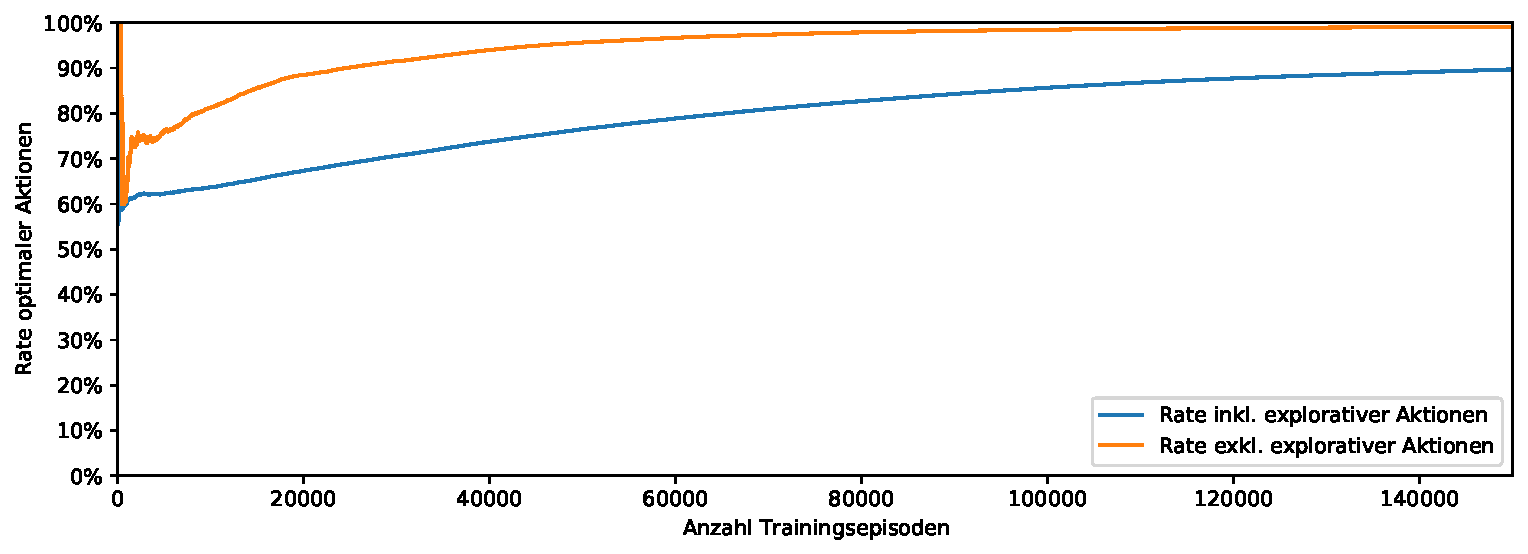
\includegraphics[scale=0.5]{convergence/convergence_compare_rate_X.pdf}
    \caption{Vergleich der Raten optimaler Aktionen}
    \label{fig:compare_rate}
\end{figure}

Um die Spielstärke der trainierten Agenten zu messen, spielt der Agent jeweils 10.000 Evaluationsspiele für beide Symbole X und O. 
Die Hyperparameter $\alpha, \epsilon$ des Agenten werden auf 0 gesetzt, damit die greedy Policy genutzt wird und kein Lernen erfolgt. 
Zum einen spielt der Agent gegen den Minimax-Algorithmus. 
Sollten mehrere Aktionen optimal sein, wählt Minimax aus dieser Menge zufällig aus, sodass unterschiedliche Zustände evaluiert werden. 
Zum anderen spielt der Agent gegen einen Spieler mit Zufallstrategie Random, damit seine Spielstärke gegen einen nicht optimalen Gegner ermittelt werden kann. 
Aufgrund von Vorexperimenten wurde festgelegt, dass fünf Agenten trainiert und das arithmetische Mittel von deren Evaluationsspielen genutzt wird, um eine bessere Vergleichbarkeit der trainierten Agenten zu ermöglichen.

Die Spielstärke kann quantifiziert werden, wenn die Spielergebnisse mit der in \cref{sec:TDL_TTT} beschriebenen Rewardfunktion bewertet werden.
In den insgesamt 20.000 Spielen gegen Minimax, kann bestenfalls ein Gesamtreward von 0 erzielt werden, da Minimax optimal spielt und das Spiel somit nur in einer Niederlage oder einem Unentschieden enden kann. 
In \cref{tab:reward_depth_penalty} wurde gezeigt, dass X frühestmöglich nach fünf und O nach sechs Zügen gewinnen kann. 
Unter der unrealistischen Annahme, dass ein Spieler jedes Spiel gegen Random in möglichst wenigen Aktionen gewinnt, beträgt der bestmögliche Reward somit 9.000, wie \cref{eq:spielstaerke_intervall} zeigt. 
Der schlechteste theoretische Wert ist -18.000 und beschreibt das Szenario, in dem jedes Spiel gegen Minimax und Random in einer schnellstmöglichen Niederlage endet.
Das Intervall der Spielstärke beträgt somit $[-18.000;9.000]$

\begin{equation}
\label{eq:spielstaerke_intervall}
\equationentry{Berechnung des Intervalls der Spielstärke}
\begin{split}
    \text{beste Spielstärke} = 20.000 \cdot 0 + 10.000 \cdot 0,5 + 10.000 \cdot 0,4 = 9.000 \\
    \text{schlechteste Spielstärke} = 20.000 \cdot -0,5 + 20.000 \cdot -0,4 = -18.000
\end{split}
\end{equation}
\chapter{Architektur und Implementierung}
In den folgenden Abschnitten wird zunächst die allgemeine Architektur der Implementierung erklärt. Anschließend werden die wichtigsten Klassen vorgestellt, sodass der Trainings- und Evaluationsprozess nachvollzogen werden können.
\section{Architektur}

\begin{figure}[h]
    \centering
    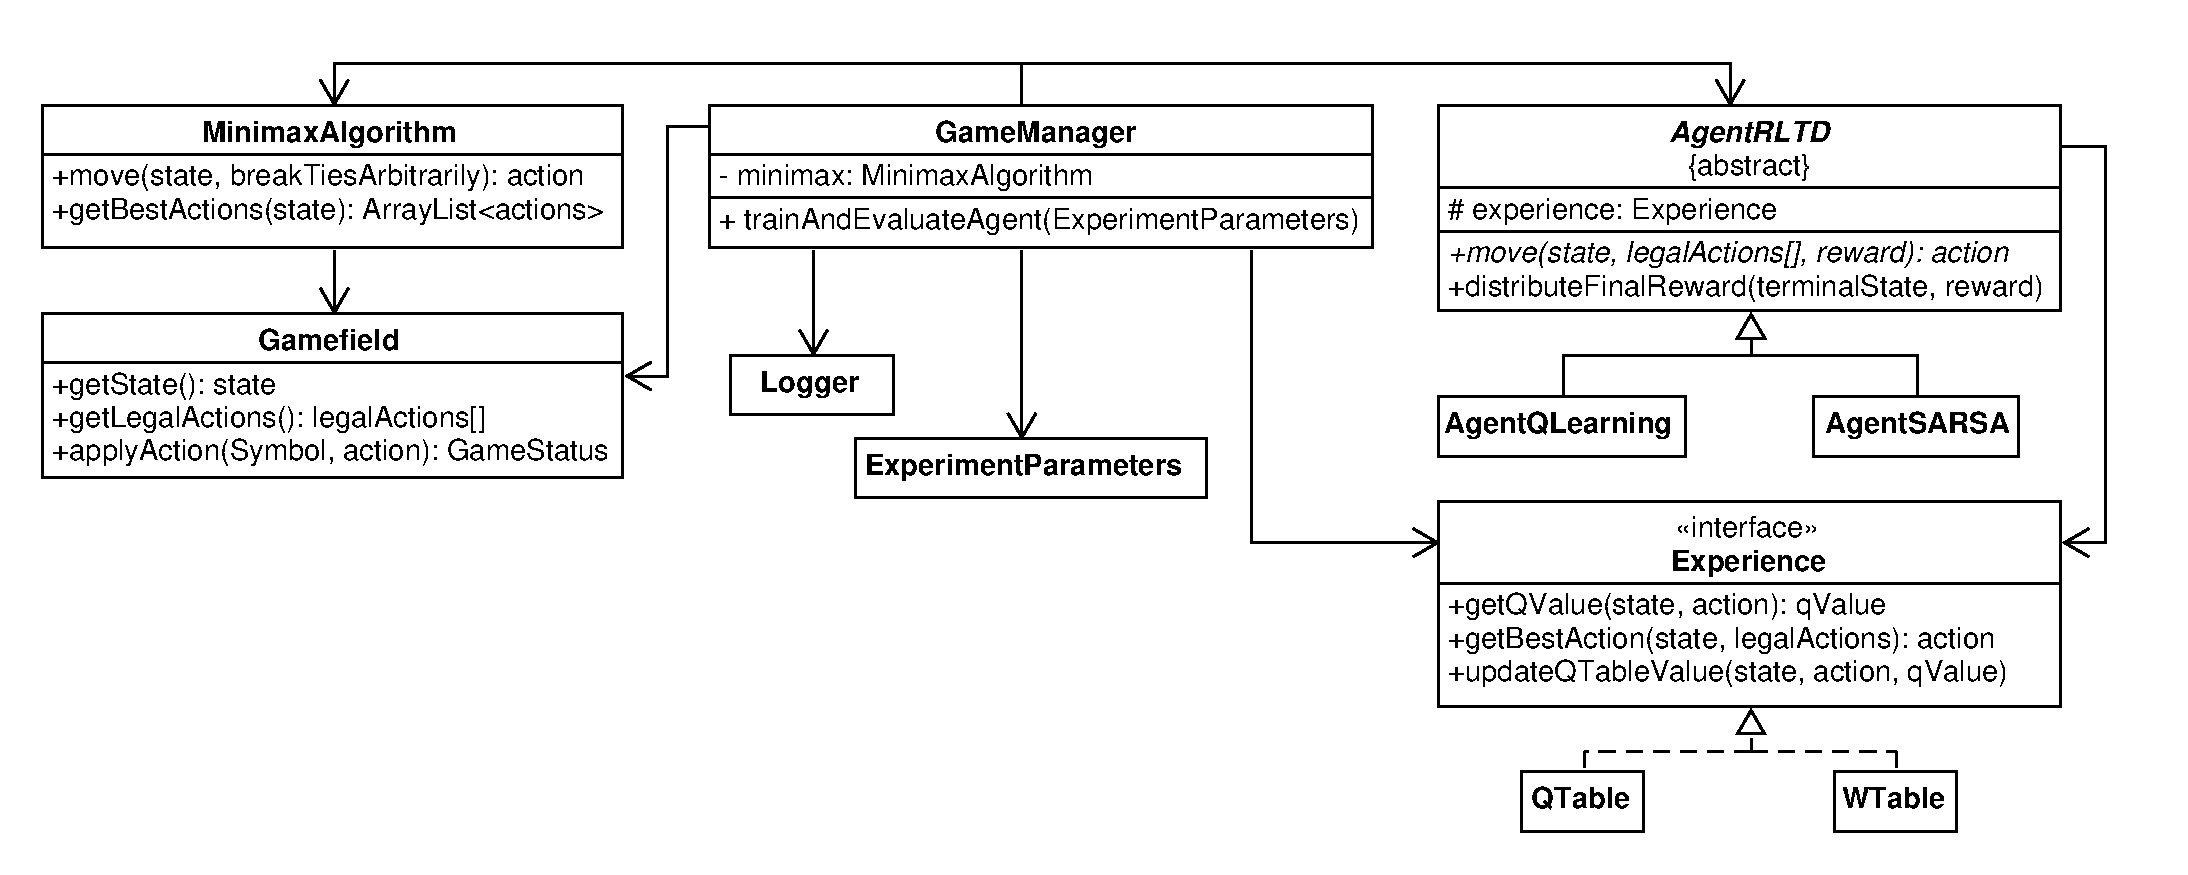
\includegraphics[width=\linewidth]{uml/uml_architektur.pdf}
    \caption{Grobe Übersicht der wichtigsten Klassen und deren Interaktion}
    \label{fig:uml_architektur}
\end{figure}

In \cref{fig:uml_architektur} ist eine Übersicht der wichtigsten Klassen.
Das UML-Diagramm stellt keinen Anspruch an Vollständigkeit, sondern dient der Vermittlung eines grundlegenden Verständnisses für die wichtigsten Bestandteile der Anwendung sowie deren Interaktion. 
Der GameManager ist die zentrale Klasse, die alle anderen Klassen verbindet, um Training und Evaluation der Agenten durchzuführen.  
Auf Basis, der in ExperimentParameters definierten Werte erstellt der GameManager zwei Agenten und weist diesen eine gemeinsame Experience Instanz zu. 
Die beiden Agenten werden mittels \splay trainiert und anschließend in Evaluationsspielen getestet. 
Zur Bewertung der Agenten verwendet der GameManager den Minimax-Algorithmus. 
Währenddessen erstellt der GameManager Log-Dateien auf deren Basis die Auswertung erfolgt.
Einerseits CSV-Dateien, die zum Plotten der Konvergenz und Berechnen der Spielstärke verwendet werden.
Zum anderen Dateien, wie im \cref{chap:meta}, die für Training und Evaluation verwendete Experimentparameter und Spielergebnisse enthalten. 
In den folgenden Abschnitten werden die Bestandteile genauer betrachtet.

Für die Implementierung wurde Java 16 und somit die derzeit aktuellste Java Version verwendet. 
Um die volle Kontrolle über die Implementierung der Agenten zu haben, wurden keine zusätzlichen Bibliotheken eingebunden. 
Die einzige Ausnahme ist die Bibliothek Apache CommonsCSV, die zur Erstellung von CSV-Dateien genutzt wird. 
Der Source-Code und die Dokumentation der Anwendung sowie Verwendungshinweise werden bereitgestellt auf \href{http://github.com/JonasBingel/ThesisHSMZ-RLTicTacToe-Java}{Github.com/JonasBingel}
\section{Gamefield}
Die Klasse Gamefield implementiert das Tic-Tac-Toe Spielfeld, wie es in \cref{chap:ttt_encoding} beschrieben wurde. 
Gamefield verwaltet pro Symbol ein Bitboard. 
Die Bitboards $B_X$ und $B_O$ wurden umgesetzt mittels der Java BitSet-Klasse, die einen Vektor von Bits verwaltet. 
Zudem implementiert die BitSet-Klasse die klassischen Logikoperationen, sodass die beschriebene Methodik zur Erfassung der legalen Aktionen und Gewinnprüfung umgesetzt werden können. 

In der Anwendung werden möglichen Aktionen und die Binärrepräsentation $B_{s}$ eines Zustands jeweils in einem int zur Basis 10 gespeichert.
Der primitve Datentyp int umfasst 32 Bits und ist somit ausreichend, um die 18 Bit von $B_{s}$ zu verwalten.  \cref{listing:getState} zeigt die Berechnung von $B_{s}$ und somit die Implementierung der \cref{eq:bitboard_bs}. 
Bevor die zu den Bitboards zugehörigen Zahlen addiert werden, erhält $B_X$ mittels LSHIFT den beschriebenen Offset von 9 Bit, d.h. der Spielfeldgröße, damit keine Überschneidung von $B_X$ und $B_O$ auftritt.

\begin{listing}[h]
\caption{getState-Methode zur Berechnung von $B_S$}
\label{listing:getState}
\inputminted{java}{04_Artefakte/03_Listings/getState.java}
\end{listing}
\section{Minimax}
\begin{figure}
    \centering
    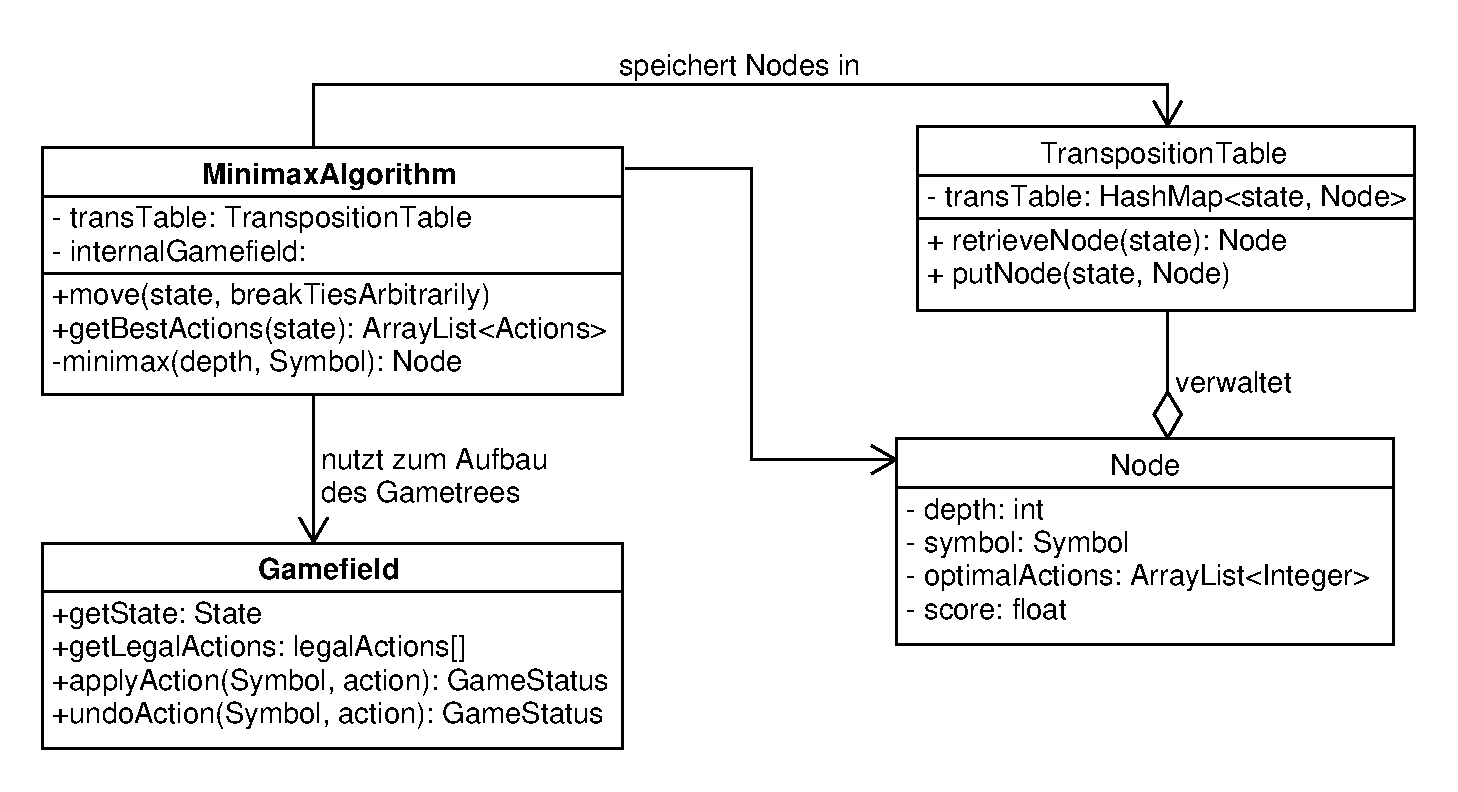
\includegraphics[width=\textwidth]{04_Artefakte/01_Abbildungen/uml/uml_minimax.pdf}
    \caption{MinimaxAlgorithm und verbundene Klassen}
    \label{fig:uml_minimax}
\end{figure}

\cref{fig:uml_minimax} zeigt die wichtigsten Bestandteile der MinimaxAlgorithm-Klasse sowie deren Interaktion mit anderen Klassen.
MinimaxAlgorithm implementiert den Minimax-Algorithmus aus \cref{sec:minimax} und dient der Evaluation der Agenten. 
Einerseits wird während des Trainings geprüft, ob die vom Agenten gewählten Aktionen optimal sind. 
Andererseits ist Minimax ein Gegner im Rahmen der Evaluationsspiele, um die Spielstärke der Agenten zu messen. 

Die Klasse bietet dafür zwei Methoden. 
Für die Bewertung der Aktionen des Agenten gibt es die getBestActions-Methode. 
Diese gibt alle gleich optimalen Aktionen zu einem Zustand zurück, sodass geprüft werden kann, ob die vom Agenten gewählte Aktion ein Element dieser Liste und somit optimal ist. 
Die move-Methode gibt für einen Zustand eine der optimalen Aktionen zurück, sodass Minimax als Gegner genutzt werden kann. 
Dabei kann als zweiter Parameter übergeben werden, ob bei mehreren gleich optimalen Aktionen die Aktion mit dem niedrigsten Index oder eine zufällige ausgewählt werden soll. 
Da in den Evaluationsspielen möglichst viele unterschiedliche Zustände betrachtet werden sollen, wird die Option für nichtdeterministisches Spiel genutzt.

Der Spielbaum wird konstruiert durch die minimax-Methode, die in Listing \cref{chap:minimax_listing} dargestellt ist. 
Mit jedem Aufruf wird ein weiterer Knoten (engl. Node) dem Spielbaum hinzufügt. 
In der minimax-Methode wird der aktuelle Zustand sowie die legalen Aktionen des intern verwalteten Spielfelds abgerufen. 
Eine der legalen Aktionen wird auf das Spielfeld angewendet und für den resultierenden Zustand wird erneut Minimax aufgerufen. 
Wird ein Terminalknoten erreicht, wird die letzte Aktion rückgängig gemacht und die nächste legale Aktion ausgeführt. 
Dies erfolgt rekursiv, bis alle Äste des Spielbaums konstruiert wurden. 
Jeder Knoten des Spielbaums entspricht einem Zustand des Spielfelds und wird repräsentiert durch eine Node-Instanz. 
Die Nodes werden unter der eindeutigen Nummer $B_{s}$ des zugehörigen Zustands in einer Transposition table gespeichert. 

Im Rahmen der Minimax-Methode werden zudem die Attribute der Node des aktuellen Zustands auf Basis der darauf folgenden Nodes aktualisiert. 
Dies beinhaltet die Anpassung der zu erwartenden Utility und die darauf basierende Auswahl der optimalen Aktionen, wobei Symbol X der maximierende und O der minimierende Spieler ist. 
Als Bewertungsfunktion verwendet Minimax ebenfalls die in \cref{sec:TDL_TTT} vorgestellte Rewardfunktion mit Depth Penalty.
\section{Reinforcement Learning Komponenten}
In den folgenden Abschnitten werden die Komponenten beschrieben, die \acl{RL} implementieren. 
Dies umfasst die Agenten für \bothAlgs sowie deren Lerndaten in Form der Q- und \wtable.

\subsection{\qlearning und \sarsa Agenten}
Da \bothAlgs eng verwandte \ac{TDL} Algorithmen sind, wurde eine abstrakte Klasse RLTDAgent erstellt, von der die konkreten Agenten abgeleitet werden. 
Neben dem Vorteil der Redundanzvermeidung nutzen AgentQLearning und AgentSARSA ein einheitliches Interface und können in den Trainings- und Evaluationsmethoden untereinander ausgetauscht werden.

Der Unterschied der beiden Algorithmen liegt in deren Vorgehen in jedem Zeitschritt, weshalb die move-Methode als abstrakt deklariert wurde. 
\cref{listing:moveQL} und \cref{listing:movesarsa} zeigen die Implementierung der move-Methode des AgentQLearning und AgentSARSA. 
Wie in \cref{chap:vergleich} erklärt, unterscheiden sie sich in zwei Aspekten. 
Einerseits in der Aktion, die jeweils für das Update verwendet wird. 
Bei \qlearning ist dies immer Aktion mit dem höchsten  \qValue und bei \sarsa die Aktion, die der Agent wirklich durchführt. 
Andererseits liegt der Unterschied darin, dass \qlearning das \ac{TD} Update durchführt, bevor es die Aktion für den Zustand $S'$ wählt. 
Da im Fall von \acs{TTT} kein Zustandswechsel möglich ist, bei dem ein Zustand $S$ sein eigener Folgezustand $S'$ ist, könnte das \acl{TD} Update auch nach der Aktionswahl durchgeführt werden. 
Dadurch reduziert sich der Unterschied auf die Wahl der Aktion für das Update. 
Auf diese Reduktion wurde verzichtet, um die Algorithmen wie vorgestellt zu implementieren und den Unterschied deutlich im Source-Code darzustellen. Beide move-Methoden implementieren die $\epsilon$-greedy-Policy \cite[S. 27f.]{suttonReinforcementLearningIntroduction2018}.

\begin{listing}[p]
\caption{move-Methode des Agent Q-Learning}
\label{listing:moveQL}
\inputminted{java}{04_Artefakte/03_Listings/move_qlearning.java}
\end{listing}

\begin{listing}[p]
\caption{move-Methode des Agent Sarsa}
\label{listing:movesarsa}
\inputminted{java}{04_Artefakte/03_Listings/move_sarsa.java}
\end{listing}

\subsection{Lerndaten}
\begin{figure}
    \centering
    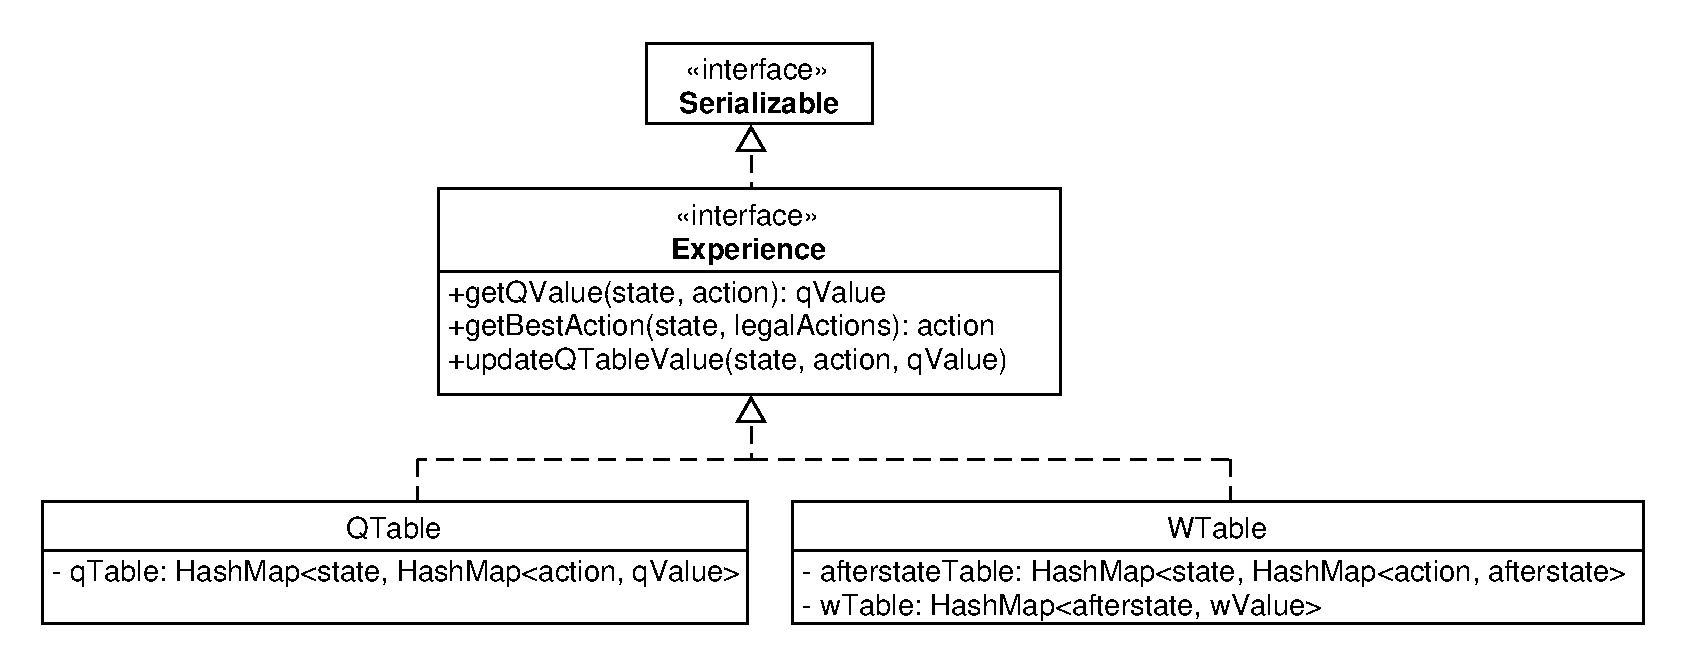
\includegraphics[width=\textwidth]{04_Artefakte/01_Abbildungen/uml/uml_experience.pdf}
    \caption{Experience Interface und implementierende Klassen}
    \label{fig:uml_experience}
\end{figure}

Die gesammelte Erfahrung des Agenten wird in der Anwendung durch das Experience Interface implementiert, das in \cref{fig:uml_experience} dargestellt ist. 
Da der Agent die Lerndaten in Form einer \qtable oder \wtable organisieren kann, bietet das Experience Interface dem Agenten einheitliche Methoden zum Zugriff auf die Lerndaten. 
Die in \cref{sec:afterstates} beschriebene Abbildung der \ac{SA Tupel} auf den resultierenden Afterstate, wird so ebenfalls vom Agenten entkoppelt und erfolgt in der Klasse WTable.

Eine Experience Instanz wird nicht durch einen Agenten selbst erzeugt, sondern im Konstruktor übergeben. 
Diese Implementierung hat zwei Gründe. 
Zum einen ist es notwendig, damit zwei Agenten im Rahmen von \splay gemeinsam eine Experience Instanz füllen können. 
Zum anderen verdeutlicht die Trennung, dass die Erfahrung kein inhärenter Bestandteil eines Agenten ist, sondern diese nur vom Agenten verwendet werden. 
Der Unterschied eines trainierten und untrainierten Agenten eines Algorithmus besteht, abgesehen von den Hyperparametern, in der Erfahrung, auf die jeweils zugegriffen wird. 
Aus diesem Grund implementiert Experience das Java Interface Serializable, wodurch Erfahrungen als Datei exportiert und importiert werden können, sodass Agenten erneut geladen werden können, um weitere Tests durchzuführen. 
In der Implementierung sind \qtable und der \afterstateTable beide mittels geschachtelten HashMaps umgesetzt, für die als Schlüssel jeweils die eindeutigen Zustände $B_{S}$ und Aktionen verwendet werden.

Im vorgestellten Pseudocode von \bothAlgs werden die \qValues aller \ac{SA Tupel} vor der ersten Episode willkürlich initialisiert. 
Dies setzt voraus, dass eine Liste aller legalen \ac{SA Tupel} vorliegt. 
Stattdessen werden in der Implementierung die \qtable und \wtable dynamisch konstruiert. 
Bei jedem Aufruf der move-Methode eines Agenten reicht dieser den aktuellen Zustand sowie die legalen Aktionen zur Initialisierung weiter. 
Dies ermöglicht die Erfassung der Zustandsanzahl, die der Agent im Rahmen des Trainings besucht hat. 
Im Konstruktor kann der initiale \qValue übergeben werden. 
In dieser Arbeit wird ausschließlich 0 verwendet. 
\section{GameManager}
Die Klasse GameManager ist zuständig für Training und Evaluation der Agenten sowie das Logging.
In \cref{fig:uml_sequence} ist der vereinfachte Ablauf des Trainings mit klassischem \splay für AgentSARSA dargestellt.
Für jedes Training wird ein neues Gamefield erzeugt und Experimentparameter definiert, auf deren Basis Experience und Agenten initialisiert werden. 
Zu Beginn jeder Episode werden die Hyperparameter der Agenten entsprechend der Experimentparameter aktualisiert. 
Anschließend wird ein Spiel gestartet und in jedem Zug werden der Zustand und die legalen Aktionen des Gamefields abgerufen. 
Beginnend mit X werden abwechselnd die move-Methoden der Agenten aufgerufen, in dessen Rahmen der direkte Reward, $r=0$, ausgegeben wird. 
Die zurückgegebene Aktion wird auf das Gamefield angewandt. 
Nach Ende des Spiels, wird der Reward mit Depth Penalty für die letzte Aktion beider Agenten verteilt und das Spielfeld zurückgesetzt. 
Das Training mit alternierendem \splay folgt dem gleichen Ablauf.
Innerhalb eines Batchs werden die Hyperparameter des nicht lernenden Agenten so gesetzt, das dieser mit der Greedy-Strategie spielt und bei Aufruf seiner move-Methode kein \ac{TD} Update durchführt.
Im Anschluss an das Training werden beide Agenten im Rahmen von Evaluationsspielen bewertet und die Experience Instanz wird als Datei serialisiert.

\begin{figure}[h]
    \centering
    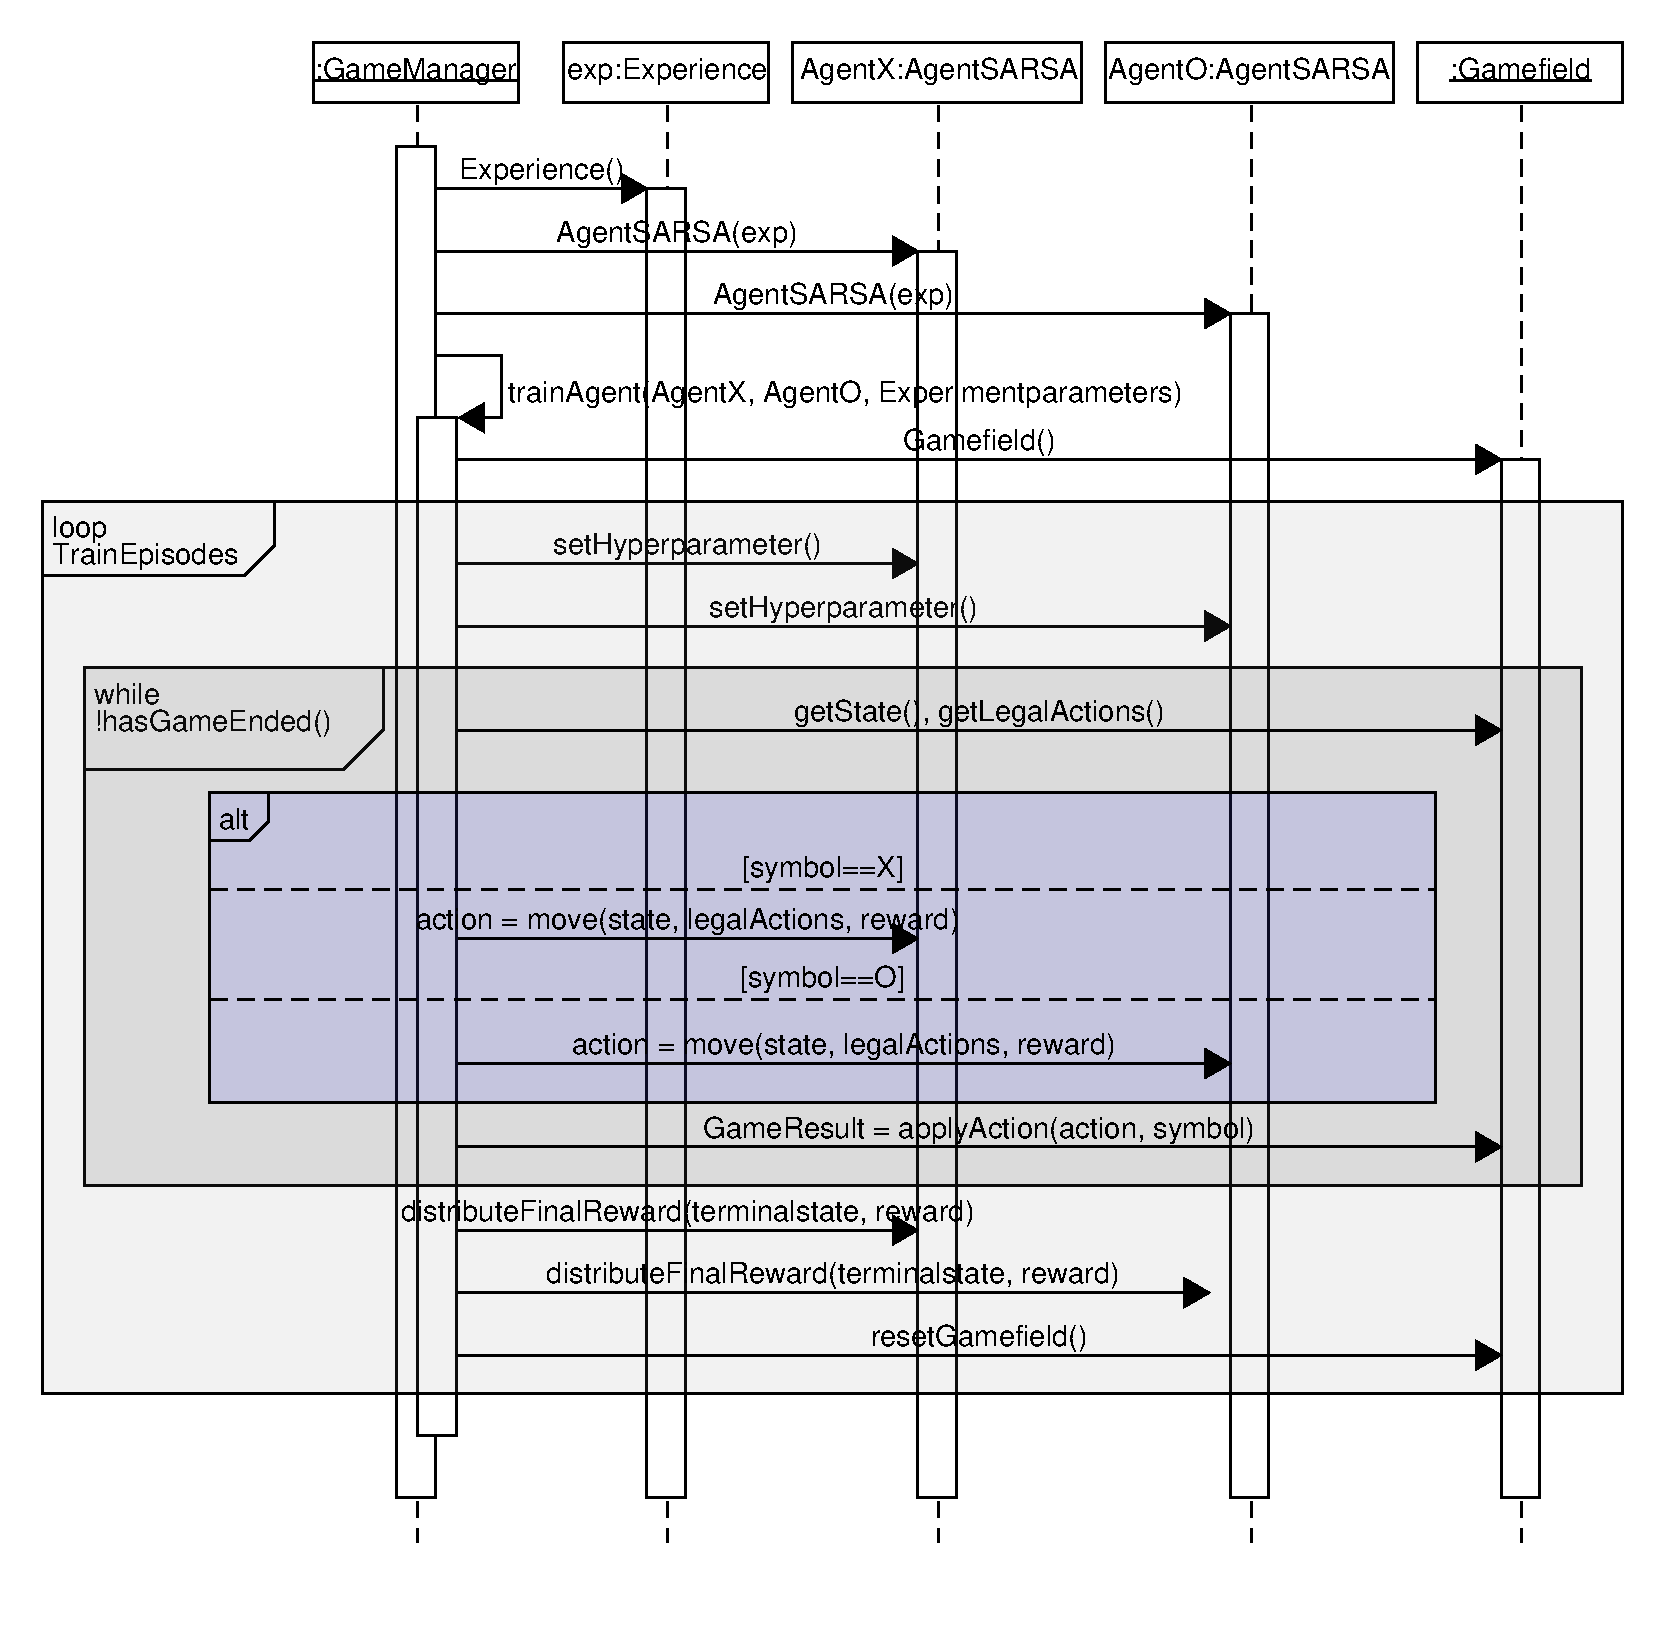
\includegraphics[width=\linewidth]{04_Artefakte/01_Abbildungen/uml/uml_sequence.pdf}
    \caption{Vereinfachte Darstellung des Trainingsablaufs mit klassischem \splay}
    \label{fig:uml_sequence}
\end{figure}
\chapter{Ergebnisse mit Auswertung und Diskussion}
In den folgenden Abschnitten werden die Ergebnisse der durchgeführten Untersuchungen vorgestellt und diskutiert. Zunächst wird ein Vergleichsmaßstab für die Spielstärke geschaffen. 
Anschließend werden die Ergebnisse von \bothAlgs vorgestellt,diskutiert und verglichen. 
Zum Schluss werden die Forschungsfragen auf Basis der Ergebnisse beantwortet.
\section{Vergleichsmaßstab der Spielstärke}
\label{sec:vergleichswerte}
Zur Evaluation spielen die trainierten Agenten jeweils 10.000 Spiele als beide Symbole gegen den Minimax-Algorithmus und einen Spieler mit Zufallsstrategie, Random. 
Damit eine Auswertung der Ergebnisse erfolgen kann, ist es zunächst notwendig einen Vergleichsmaßstab zu schaffen. 
Dafür spielen die Evaluationsgegner, Minimax-Algorithmus und Random, selbst gegeneinander.

\cref{tab:resultmatrix_baseline} enthält die Spielergebnisse jeder Kombination von Minimax und Random.
Die dargestellten Ergebnisse sind das arithmetische Mittel von fünf Durchläufen und konsistent zu den Experimenten in \cite{mirnovi.QLearningTicTacToe2020}.
Minimax spielt gegen sich selbst immer zu einem Unentschieden und gewinnt gegen Random in 97\% der Spiele als X und 78\% der Spiele als O.
Minimax kann gegen Random nicht immer gewinnen, da die Wahrscheinlichkeit besteht, dass Random zufällig optimale Aktionen wählt und das Spiel so in einem Unentschieden endet.

Aus den Testspielen kann zudem die durchschnittliche Wahrscheinlichkeit berechnet werden, mit der eine zufällig gewählte Aktion laut Minimax optimal ist. 
Für das Symbol X beträgt die Wahrscheinlichkeit ungefähr 70\% und für das Symbol O knapp 38\%. 
Die Wahrscheinlichkeit ist abhängig vom Symbol, da beispielsweise laut Minimax jede erste Aktion von X optimal ist. Hingegen muss O bereits in seiner ersten Aktion einen Konter für die Aktion von X wählen. Dies erklärt zudem, wieso im Szenario Random gegen Random das Symbol X mehr als die Hälfte der Spiele gewinnt. Basierend auf diesen Spielergebnissen wurde die Spielstärke beider Evaluationsgegner berechnet. 
Wie in \cref{sec:eval_metrik} beschrieben, ist das Intervall der Spielstärke $[-18.000;9.000]$. 
Minimax erreicht eine Spielstärke von $6917,86 \pm 22,29$ und Random von $-6938 \pm34,67$.

\begin{table}
\centering
\caption{Spielergebnismatrix von Minimax und Spieler mit Zufallsstrategie Random}
\label{tab:resultmatrix_baseline}

\begin{tabular}{llrlr}
\toprule
 & \multicolumn{2}{l}{\textbf{X Minimax}} & \multicolumn{2}{l}{\textbf{X Random}} \\ \midrule
\textbf{O Minimax}  & X Minimax:        & 0,00\% $\pm$    0,00\%            & X Random:         & 0,00\% $\pm$ 0,00\%  \\
                    & O Minimax:        & 0,00\% $\pm$    0,00\%            & O Minimax:        & 77,63\% $\pm$ 4,91\%  \\
                    & Unentschieden:    & 100,00\% $\pm$  0,00\%            & Unentschieden:    & 22,37\% $\pm$ 4,91\%  \\ \cmidrule{2-5}
\textbf{O Random}   & X Minimax:        & 0,00\% $\pm$    0,00\%            & X Random:         & 58,38\% $\pm$ 5,41\%  \\
                    & O Random:         & 0,00\% $\pm$    0,00\%            & O Random:         & 29,00\% $\pm$ 1,91\%  \\
                    & Unentschieden:    & 100,00\% $\pm$  0,00\%            & Unentschieden:    & 12,62\% $\pm$ 3,95\%  \\ \bottomrule
\end{tabular}
\end{table}

\section{Auswertung des \qlearning Agenten}
In den folgenden Abschnitten werden die Ergebnisse der Q-Learning Agenten vorgestellt und ausgewertet. Zunächst wird die Konvergenz während dem Training und die Spielstärke betrachtet. Anschließend wird vorgestellt, welche Auswirkung die Nutzung von Afterstates hat. Abschließend erfolgt eine Detailbetrachtung für ausgewählte Zustände.

\subsection{Konvergenz der Rate optimaler Aktionen}
\begin{figure}
\centering
\begin{subfigure}[b]{0.75\textwidth}
    \centering
   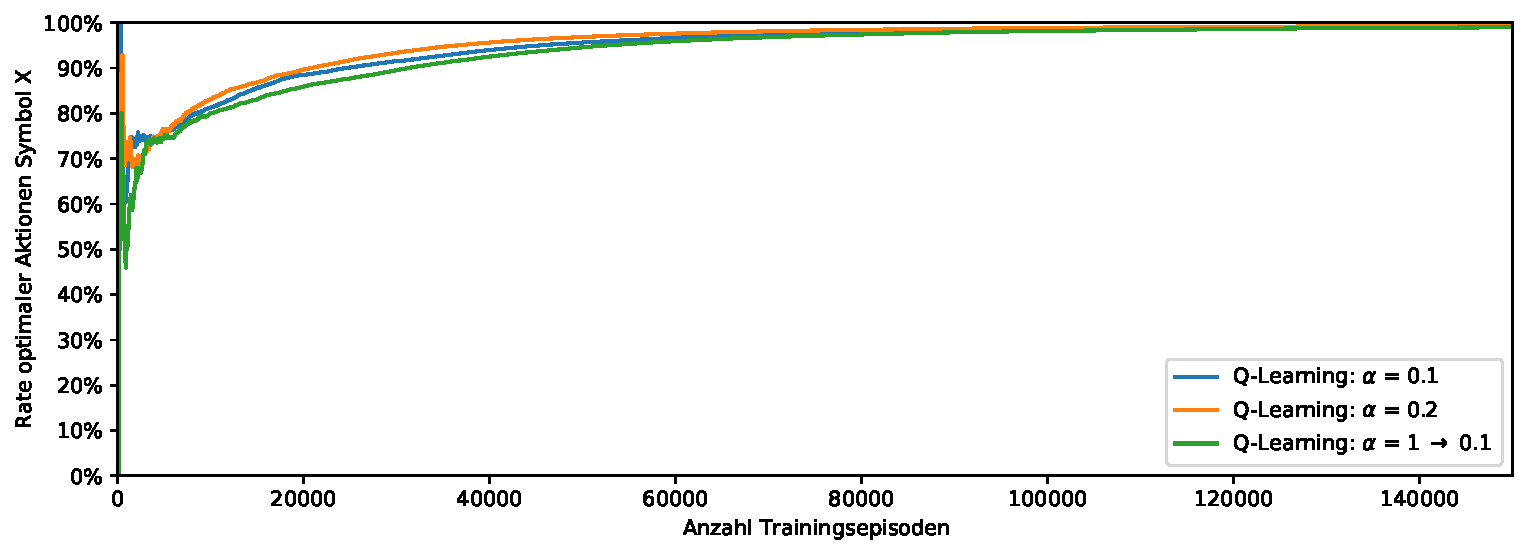
\includegraphics[width=1\linewidth]{convergence/convergence_compare_alpha_QLearning_X.pdf}
   \caption{Symbol X}
   \label{fig:convergence_compare_alpha_QLearning_X} 
\end{subfigure}

\begin{subfigure}[b]{0.75\textwidth}
    \centering
   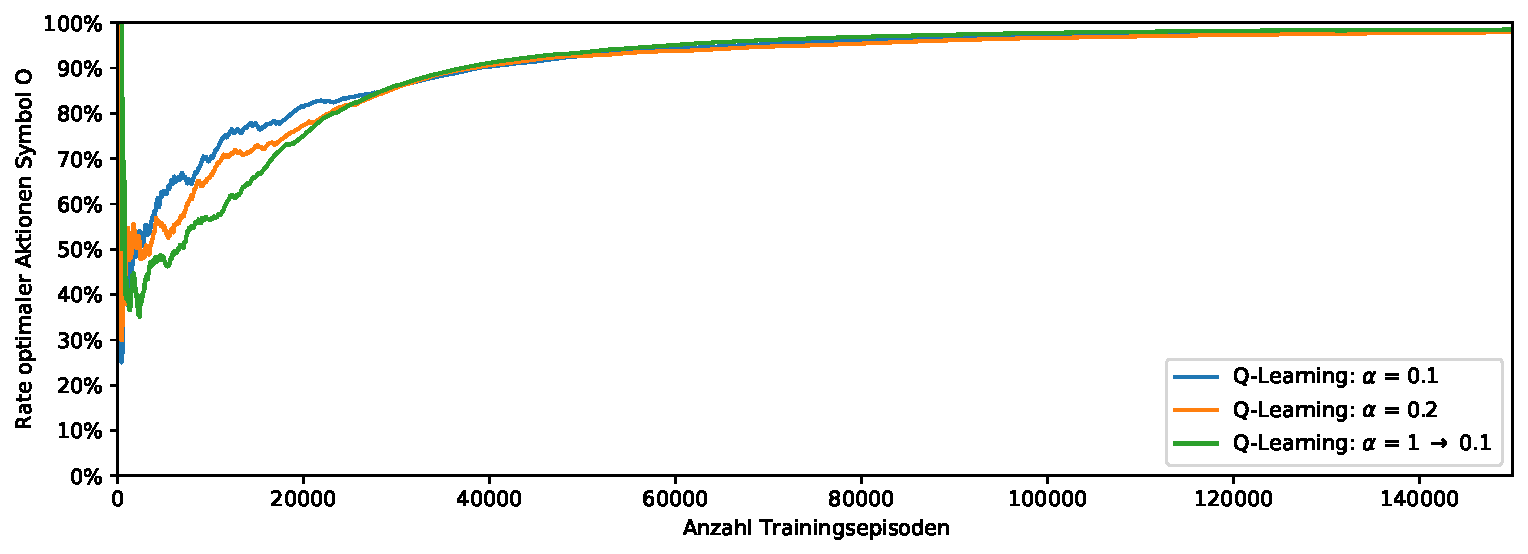
\includegraphics[width=1\linewidth]{convergence/convergence_compare_alpha_QLearning_O.pdf}
   \caption{Symbol O}
   \label{fig:convergence_compare_alpha_QLearning_O}
\end{subfigure}

\caption[Rate optimaler Aktionen Q-Learning unterschiedliche Lernraten, klassisches \splay]{Rate optimaler Aktionen von Q-Learning für verschiedene Lernraten $\alpha$, klassisches \splay (a) Symbol X (b) Symbol O}
\label{fig:convergence_compare_alpha_QLearning}
\end{figure}


\cref{fig:convergence_compare_alpha_QLearning} zeigt den Verlauf der Rate optimaler Aktionen der \qlearning Agenten mit den drei verschiedenen Lernraten $\alpha$ währen des Trainings mit klassischem \splay. 
Die drei Graphen für Symbol X unterscheiden sich stärker innerhalb der ersten 5.000 Episoden. 
Ab ungefähr 70.000 Episoden ist die Rate stabil, wobei $\alpha = 0,2$ am schnellsten konvergiert, dicht gefolgt von $\alpha=0,1$. 
Im Gegensatz dazu unterscheiden sich die Graphen für Symbol O deutlich stärker und verlaufen erst ab ungefähr 30.000 Episoden gleich. 
Zudem beginnt die Rate für Symbol O etwas über 0,4 und ist somit niedriger als die Rate von X.
Dies kann erklärt werden durch die unterschiedliche Wahrscheinlichkeit zufällig eine optimale Aktion zu wählen, wie \cref{sec:vergleichswerte} beschrieben. 
Ab ungefähr 100.000 Episoden stabilisiert sich die Rate für das Symbol O auf einem niedrigeren Wert als X. 
Somit konvergiert Symbol O langsamer als Symbol X, wobei Symbol O für $\alpha = 0,1$  am schnellsten konvergiert. 
Da die Agenten durch \splay trainiert werden und somit beide Symbole spielen, muss die Konvergenzrate auch für beide Symbole gemeinsam betrachtet werden. 
Daher konvergiert \qlearning bei klassischem \splay für $\alpha=0,1$ am schnellsten. 

Der Vergleich der Rate optimaler Aktionen von \qlearning für alternierendes \splay ist im \cref{chap:app_qlearning}. 
Für beide Symbole konvergiert alternierendes \splay langsamer als das klassische \splay und stabilisiert sich auf einer geringeren Rate.

\subsection{Spielstärke}

\cref{tab:playingAbility_ql_normal} und \cref{tab:playingAbility_ql_alternate} zeigen die durchschnittliche Spielstärke der trainierten Agenten für klassisches und alternierendes \splay. 
Alle Agenten, die mit klassischem \splay trainiert wurden, erreichen eine bessere durchschnittliche Spielstärke als Minimax. 
Im Gegensatz dazu ist die durchschnittliche Spielstärke aller Agenten, die mit alternierendem \splay trainiert wurden schlechter als die des Minimax und deutlich schlechter im Vergleich zum klassischen \splay.

Der \qlearning Agent, der die Lernrate $\alpha=0,1$ nutzt und mit klassischem \splay trainiert wurde, konvergierte am schnellsten und erreicht mit durchschnittlich 8.002,72 die höchste Spielstärke.
\cref{tab:resultmatrix_ql_normal_alpha01} enthält die Spielergebnisse der Evaluationsspiele dieses Agenten. 
Der Agent spielt perfekt gegen Minimax sowohl als Symbol X als auch Symbol O. 
Gegen Random verliert der Agent keine Spiele und erreicht eine Gewinnrate als Symbol X von 99\% und Symbol O von 91\%. 
Die Gewinnrate ist somit besser als die von Minimax, die 97\% bzw. 78\% beträgt. 
Somit konnte \qlearning durch \splay lernen, \ac{TTT} gegen Gegner unterschiedlicher Spielstärke erfolgreich zu spielen. 
Die Spielergebnismatrizen des \qlearning Agenten für die anderen Hyperparameter und Arten von\splay sind im \cref{chap:app_qlearning} angegeben.

\begin{table}
\centering
\caption[Spielstärke Q-Learning unterschiedliche Lernraten, klassisches \splay]{Spielstärke von Q-Learning mit unterschiedlichen Lernraten, klassisches \splay}
\label{tab:playingAbility_ql_normal}

% change color with \textcolor{red}{text}
\begin{tabular}{lrrr}
\toprule
Lernrate $\alpha$ &  Spielst"arke Q-Learning & Spielst"arke Minimax & Differenz zu Minimax \\ \midrule
Konstant 0,1                    & 8.002,72 $\pm$ \phantom{0}30,03   & 6.917,86  & 1.084,86 $\pm$ \phantom{0}30,03 \\
Konstant 0,2                    & 7.801,36 $\pm$ 131,22             & 6.917,86  & 883,5 $\pm$ 131,22 \\
Abnehmend 1 $\rightarrow$ 0,1   & 7.894,92 $\pm$ 132,52             & 6.917,86  & 977,06 $\pm$ 132,52 \\ \bottomrule

\end{tabular}

\end{table}
\begin{table}
\centering
\caption[Spielstärke Q-Learning unterschiedliche Lernraten, alternierendes \splay]{Spielstärke von Q-Learning mit unterschiedlichen Lernraten, alternierendes \splay}
\label{tab:playingAbility_ql_alternate}

\begin{tabular}{lrrr}
\toprule
Lernrate $\alpha$ &  Spielst"arke Q-Learning & Spielst"arke Minimax & Differenz zu Minimax \\ \midrule
Konstant 0,1                    & 6.465,66 $\pm$ 481,99             & 6.917,86  & \textcolor{red}{-452,2 $\pm$ 481,99} \\
Konstant 0,2                    & 6.904,92 $\pm$ 399,15             & 6.917,86  & \textcolor{red}{-12,94 $\pm$ 399,15} \\
Abnehmend 1 $\rightarrow$ 0,1   & 6.110,56 $\pm$ 224,66             & 6.917,86  & \textcolor{red}{-807,3 $\pm$ 224,66} \\ \bottomrule

\end{tabular}
\end{table}
\begin{table}
\centering
\caption[Spielergebnismatrix \qlearning: $\alpha=0,1$, klassisches \splay]{Spielergebnismatrix für \qlearning mit Lernrate $\alpha=0,1$, klassisches \splay}
\label{tab:resultmatrix_ql_normal_alpha01}

\begin{tabular}{llrlr}
\toprule
 & \multicolumn{2}{l}{\textbf{Minimax}} & \multicolumn{2}{l}{\textbf{Random}} \\ \midrule
\textbf{X Q-Learning}   & X Q-Learning:     & 0,00\% $\pm$    0,00\%            & X Q-Learning:         & 99,22\% $\pm$ 0,37\%  \\
                        & O Minimax:        & 0,00\% $\pm$    0,00\%            & O Random:            & 0,00\% $\pm$ 0,00\%  \\
                        & Unentschieden:    & 100,00\% $\pm$  0,00\%            & Unentschieden:        & 0,78\% $\pm$ 0,37\%  \\ \cmidrule{2-5}
\textbf{O Q-Learning}   & X Minimax:        & 0,00\% $\pm$    0,00\%            & X Random:             & 0,00\% $\pm$ 0,00\%  \\
                        & O Q-Learning:     & 0,00\% $\pm$    0,00\%            & O Q-Learning:         & 91,45\% $\pm$ 0,21\%  \\
                        & Unentschieden:    & 100,00\% $\pm$  0,00\%            & Unentschieden:        & 8,55\% $\pm$ 0,21\%  \\ \bottomrule
\end{tabular}
\end{table}

\subsection{\wtable}
Zur Evaluation der Auswirkung von Afterstates auf die Konvergenz und Spielstärke wird der stärkste ermittelte \qlearning Agent mit einem Agenten verglichen, der eine \wtable und die gleichen Hyperparameter nutzt. 
Wie im vorigen Abschnitt beschrieben, ist dies ein \qlearning Agent mit Lernrate $\alpha=0,1$, der mit klassischen \splay trainiert wird.

\cref{fig:convergence_compare_experience_QLearning} vergleicht die Rate optimaler Aktionen von Agenten mit \qtable und mit \wtable. 
Sowohl für Symbol X als auch Symbol O konvergiert der Agent mit \wtable deutlich schneller und stabilisiert sich auf einer höheren Rate optimaler Aktionen. 
Dies äußert sich in der Spielstärke des Agenten, wie \cref{tab:resultmatrix_ql_normal_alpha01_afterstate} zeigt.

Durch die Nutzung des \wtable im Vergleich zur \qtable steigert sich die durchschnittliche Gewinnrate gegen Random als Symbol X von 99,22\% auf 99,46\% und als Symbol O von 91,45\% auf 91,51\%.
Die absolute Spielstärke steigt von 8.002,72 auf 8.036,68. 
Dies könnte wie in \cref{sec:afterstates} und \cite[S. 136f.]{suttonReinforcementLearningIntroduction2018} beschrieben, auf die effektivere Nutzung der gesammelten Erfahrung zurückgeführt werden.
Da die Spielstärke der Spielstärke für den \qtable jedoch $\pm 75,69$ beträgt und die Stichprobenanzahl mit $N=5$ klein ist, kann dies nicht sicher gesagt werden.
Es ist daher auch möglich, dass die Verbesserung durch Zufall entstanden somit statistisch nicht signifikant ist.

Die ermittelten Spielergebnisse des \qlearning Agenten sind konsistent mit anderen Experimenten in \cite{mirnovi.QLearningTicTacToe2020}. 
In diesen wurde jedoch ein Double \qlearning Agent mit \qtable und abnehmenden Hyperparametern durch klassisches Self-play für 3.000.000 Episoden trainiert.

\begin{figure}
\centering
\begin{subfigure}[b]{0.75\textwidth}
    \centering
   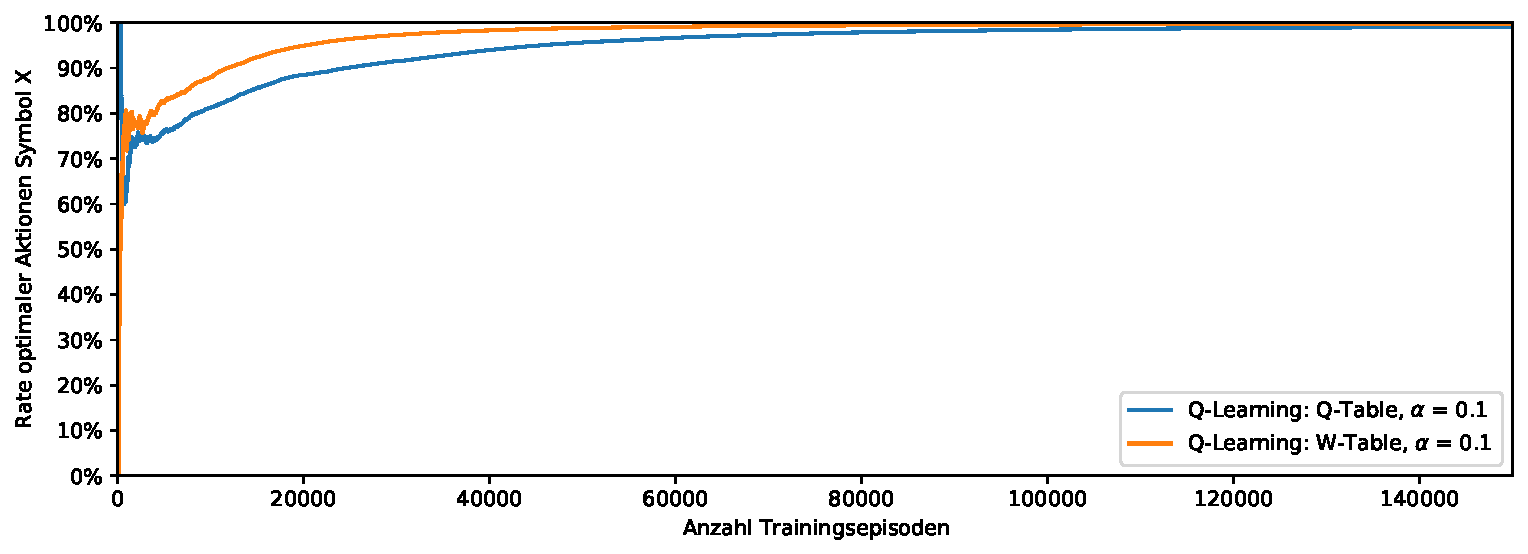
\includegraphics[width=1\linewidth]{convergence/convergence_compare_experience_QLearning_X.pdf}
   \caption{Symbol X}
   \label{fig:convergence_compare_experience_QLearning_X} 
\end{subfigure}

\begin{subfigure}[b]{0.75\textwidth}
    \centering
   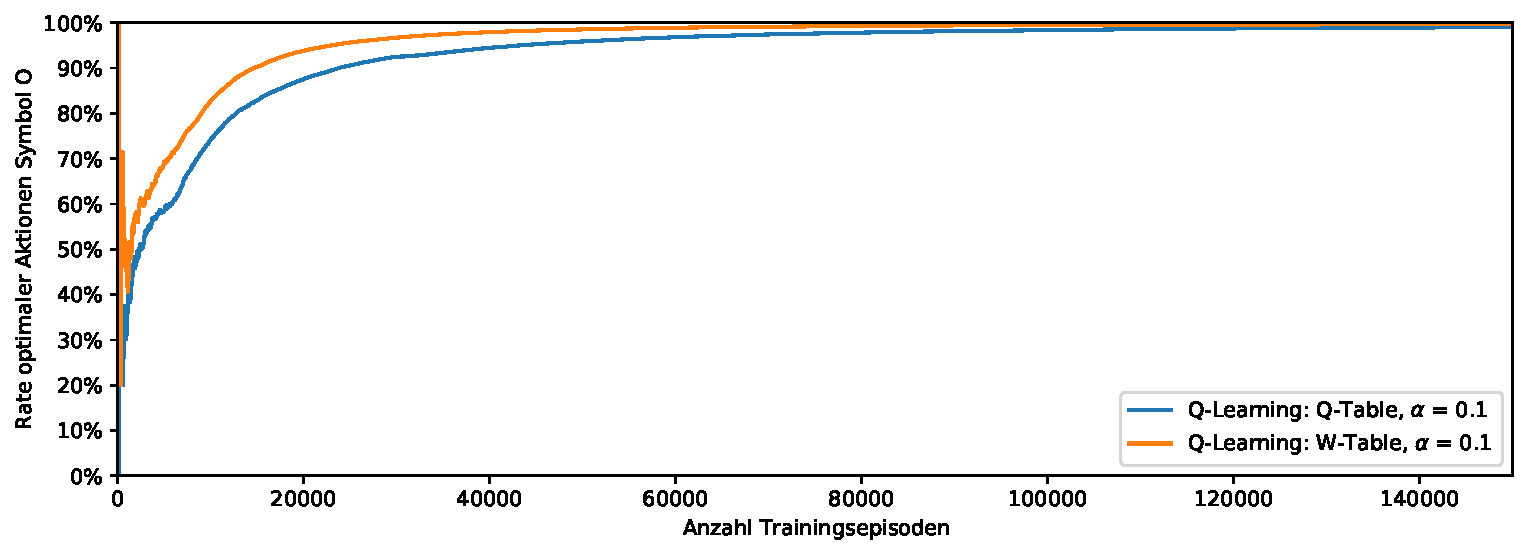
\includegraphics[width=1\linewidth]{convergence/convergence_compare_experience_QLearning_O.pdf}
   \caption{Symbol O}
   \label{fig:convergence_compare_experience_QLearning_O}
\end{subfigure}

\caption[Rate optimaler Aktionen bester Q-Learning Agent, \wtable, klassisches \splay]{Rate optimaler Aktionen von Q-Learning Lernrate $\alpha=0,1$, \wtable, klassisches \splay (a) Symbol X (b) Symbol O}
\label{fig:convergence_compare_experience_QLearning}
\end{figure}

\begin{table}
\centering
\caption[Spielergebnismatrix Q-Learning: $\alpha=0,1$, \wtable, klassisches \splay]{Spielergebnismatrix für \qlearning mit Lernrate $\alpha=0,1$ und \wtable, klassisches \splay}
\label{tab:resultmatrix_ql_normal_alpha01_afterstate}

\begin{tabular}{llrlr}
\toprule
 & \multicolumn{2}{l}{\textbf{Minimax}} & \multicolumn{2}{l}{\textbf{Random}} \\ \midrule
\textbf{X Q-Learning}   & X Q-Learning:     & 0,00\% $\pm$    0,00\%            & X Q-Learning:         & 99,46\% $\pm$ 0,05\%  \\
                        & O Minimax:        & 0,00\% $\pm$    0,00\%            & O Random:            & 0,00\% $\pm$ 0,00\%  \\
                        & Unentschieden:    & 100,00\% $\pm$  0,00\%            & Unentschieden:        & 0,54\% $\pm$ 0,05\%  \\ \cmidrule{2-5}
\textbf{O Q-Learning}   & X Minimax:        & 0,00\% $\pm$    0,00\%            & X Random:             & 0,00\% $\pm$ 0,00\%  \\
                        & O Q-Learning:     & 0,00\% $\pm$    0,00\%            & O Q-Learning:         & 91,51\% $\pm$ 0,20\%  \\
                        & Unentschieden:    & 100,00\% $\pm$  0,00\%            & Unentschieden:        & 8,49\% $\pm$ 0,20\%  \\ \bottomrule
\end{tabular}
\end{table}

\subsection{Detailbetrachtung}
Die Spielstärke des \qlearning Agenten wirft die Frage auf, wie der Agent besser als ein Minimax-Algorithmus spielen kann. 
Wie in \cref{sec:minimax} erwähnt, erwartet der  Minimax-Algorithmus einen optimalen Gegner und spielt nur gegen diesen optimal. 
Hingegen hat \qlearning auch gelernt gegen nicht optimale Gegner optimal zu spielen.
Dies wird deutlich, wenn die Einträge der \qtable \bzw \wtable für einen Zustand betrachtet werden. 
\cref{ttt_boards/ttt_6754} zeigt das Spielfeld des Zustands $6754$ und \cref{tab:state6754} die Bewertung der legalen Aktionen durch den Minimax und \qlearning Agent mit \wtable. 
In diesem Zustand ist Symbol X am Zug und die laut Expert Play optimalen Aktionen sind 4 und 8, um den Gegner zum Blocken zu zwingen. 
Wählt Symbol O im nächsten Zug die nicht optimale Aktion 7, gewinnt X. 
Die Aktion 7 garantiert hingegen, dass das Spiel unentschieden endet. 
Minimax weist allen Aktionen den Wert 0 zu, da dieser von einem optimalen Gegner und somit einem Unentschieden ausgeht. 
Der \qlearning Agent weist den Aktionen 4 und 8 einen positiven Wert zu, da im Rahmen des Trainings auch gegen nicht optimale Gegner gespielt wurde und so Erfahrungen vorliegen, in denen der Agent das Spiel aus diesem Zustand gewonnen hat. 

\begin{minipage}{\textwidth}
  \begin{minipage}[b]{0.49\textwidth}
    \centering
    \captionsetup{type=figure}
    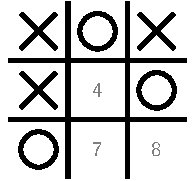
\includegraphics[]{ttt_boards/ttt_6754.pdf}
    \captionof{figure}{Spielfeldkonstellation Zustand 6754}
    \label{ttt_boards/ttt_6754}
  \end{minipage}
  \hfill
  \begin{minipage}[b]{0.49\textwidth}
    \centering
        \captionsetup{type=table}
    %\begin{table}
%\centering
%\caption{Bewertung Aktionen in State $6754_{10}$ bester Q-Learning Agent mit Lernrate $\alpha$ =0,1 und W-Table}
\begin{tabular}{lll}
\toprule
Aktion  & Minimax & Q-Learning \\ \midrule
4	    & 0	                & 0,0015 \\
7   	& 0	                & 0,0000 \\
8	    & 0	                & 0,0006 \\ \bottomrule
\end{tabular}
%\end{table}
    \captionof{table}{Bewertung Aktionen in Zustand 6754}
    \label{tab:state6754}
    \end{minipage}
\end{minipage}

Eine Forschungsfrage ist die Ermittlung der besten ersten Aktion für das Symbol X. 
Zur Beantwortung soll die Bewertung des besten \qlearning Agenten für alle legalen Aktionen im Zustand $0$ betrachtet werden. 
\cref{tab:state0_eval_ql} listet die durchschnittliche Bewertung der Aktionen von fünf \qlearning Agenten mit \wtable. 
Die Aktion 4 (Mitte) hat mit 0,0053 den höchsten \qValue. 
Jedoch zeigt die Auflistung der \qValues ein weiteres Problem.  
Die Tabelle enthält jeweils vier Bewertungen für Ecken und Kanten, die alle den gleichen Wert haben sollten. 
Die Aktionen sollten den gleichen Wert haben, da sie in Zuständen resultieren, die nach Rotation oder Spiegelung äquivalent sind. 
Durch Berechnung der durchschnittlichen Bewertung je äquivalenter Aktion, wie in \cref{tab:state0_eval_ql_aggregated}, kann die durchschnittliche Rangfolge der Aktionen angegeben werden. 
Demnach ist die Aktion Mitte weiterhin die beste Aktion, gefolgt von der Aktion Ecke. 
Für eine abschließende Beantwortung der Frage wäre eine Enkodierung der Zustände notwendig, die äquivalenten Zuständen einen gemeinsamen Bezeichner und \qValue zuweist. 
Das Ergebnis, dass die beste erste Aktion die Mitte ist, ist jedoch konsistent zu vorher durchgeführten Experimenten von \cite{kutscheraa.BestOpeningMove2018}.

\begin{table}[!htb]
    \begin{minipage}[t]{.5\textwidth}
        \centering
        \caption{Bewertung Zustand 0 \\ bester Q-Learning Agent}
        \label{tab:state0_eval_ql}
        \begin{tabular}{lr}
        \toprule
        Aktion  & Bewertung \\ \midrule
        0       & 0,0041 \\
        1       & 0,0041 \\
        2		& 0,0045 \\
        3		& 0,0033 \\
        4		& 0,0053 \\
        5		& 0,0030 \\
        6		& 0,0035 \\
        7		& 0,0033 \\
        8		& 0,0044 \\ \bottomrule
    \end{tabular}
    \end{minipage}%
    \begin{minipage}[t]{.5\textwidth}
        \centering
        \caption{Bewertung Aktionsklassen Zustand 0 bester Q-Learning Agent}
        \label{tab:state0_eval_ql_aggregated}
        \begin{tabular}{lr}
        \toprule
        Aktion  & Bewertung \\ \midrule
        Ecke	& 0,0041 \\
        Kante	& 0,0034 \\
        Mitte	& 0,0053 \\ \bottomrule
        \end{tabular}
    \end{minipage}
\end{table}
\section{Auswertung des \sarsa Agenten}
In den folgenden Abschnitten werden die Ergebnisse der Sarsa Agenten vorgestellt und ausgewertet. Zunächst wird die Konvergenz während dem Training und die Spielstärke betrachtet. Anschließend wird vorgestellt, welche Auswirkung die Nutzung von Afterstates hat. Abschließend erfolgt eine Detailbetrachtung für ausgewählte Zustände.
\subsection{Konvergenz der Rate optimaler Aktionen}

\begin{figure}
\centering
\begin{subfigure}[b]{0.75\textwidth}
    \centering
   \includegraphics[width=1\linewidth]{convergence/convergence_compare_alpha_sarsa_X.pdf}
   \caption{Symbol X}
   \label{fig:convergence_compare_alpha_sarsa_X} 
\end{subfigure}

\begin{subfigure}[b]{0.75\textwidth}
    \centering
   \includegraphics[width=1\linewidth]{convergence/convergence_compare_alpha_sarsa_O.pdf}
   \caption{Symbol O}
   \label{fig:convergence_compare_alpha_sarsa_O}
\end{subfigure}

\caption[Rate optimaler Aktionen \sarsa unterschiedliche Lernraten, klassisches \splay]{Rate optimaler Aktionen von \sarsa für verschiedene Lernraten $\alpha$, klassisches \splay (a) Symbol X (b) Symbol O}
\label{fig:convergence_compare_alpha_sarsa}
\end{figure}

\cref{fig:convergence_compare_alpha_sarsa} zeigt den Verlauf der Rate optimaler Aktionen von \sarsa Agenten mit den drei verschiedenen Lernraten $\alpha$ während des Trainings mit klassischem \splay. 
Der Agent mit Lernrate $\alpha=0,1$ konvergiert am schnellsten, dicht gefolgt von $\alpha=0,2$. 
Für das Symbol X stabilisiert sich die Rate ab ungefähr 90.000 und für O ab 110.000 Trainingsepisoden. 

Die Agenten von Symbol X stabilisieren sich auf einer höheren Rate optimaler Aktionen als die von Symbol O, wobei in beiden Fällen der Agent mit $\alpha=0,1$ die höchste Rate erreicht. 
Hingegen konvergiert bei beiden Symbolen der Agent mit abnehmender Lernrate langsamer und erreicht, insbesondere bei Symbol O, eine niedrigere Rate optimaler Aktionen.

Der Vergleich der Rate optimaler Aktionen von \sarsa für alternierendes \splay ist im \cref{chap:app_sarsa}. 
Für beide Symbole konvergiert das alternierende \splay langsamer als das klassische \splay und stabilisiert sich auf einer geringeren Rate.


\subsection{Spielstärke}
\cref{tab:playingAbility_sarsa_normal} und \cref{tab:playingAbility_sarsa_alternate} zeigen die durchschnittliche Spielstärke der trainierten Agenten für klassisches und alternierendes \splay. Für beide Arten von \splay erreichen die Agenten eine durchschnittliche Spielstärke, die über der des Minimax liegt. 
Die einzige Ausnahme sind Agenten, die mit konstanter Lernrate $\alpha=0,1$ durch alternierendes \splay trainiert wurden und eine durchschnittliche Spielstärke von 6.496,50 haben. 
Training durch klassisches \splay resultiert für \sarsa in stärkeren Agenten als Training durch alternierendes \splay. 
Der \sarsa Agent, der die Lernrate $\alpha=0,1$ nutzt und mit klassischem \splay trainiert wurde erreicht mit 7.905,72 die höchste Spielstärke. 

\cref{tab:resultmatrix_sarsa_normal_alpha01} enthält die Spielergebnisse der Evaluationsspiele des stärksten \sarsa Agenten. 
Als Symbol X spielt der \sarsa Agent optimal gegen Minimax. 
Zudem gewinnt der Agent 99\% der Spiele gegen Random und somit mehr als der Minimax, der nur 97\% gewinnt. 
Als Symbol O gewinnt der Agent mit 89\% mehr Spiele gegen Random als Minimax, der nur eine Gewinnrate von 78\% erreicht.
Jedoch verliert der Agent als Symbol O 0,74\% der Evaluationsspiele gegen Minimax und 0,11\% gegen Random.
Somit erreicht der Agent eine höhere Spielstärke als Minimax, spielt jedoch nicht optimal. 
Die Spielergebnismatrizen der \sarsa Agenten für die anderen Hyperparameter und Arten von \splay sind im \cref{chap:app_sarsa} angegeben.

\begin{table}
\centering
\caption[Spielstärke \sarsa unterschiedliche Lernraten, klassisches \splay]{Spielstärke von \sarsa mit unterschiedlichen Lernraten, klassisches \splay}
\label{tab:playingAbility_sarsa_normal}

% change color with \textcolor{red}{text}
\begin{tabular}{lrrr}
\toprule
Lernrate $\alpha$ &  Spielst"arke Sarsa & Spielst"arke Minimax & Differenz zu Minimax \\ \midrule
Konstant 0,1                    & 7.905,72 $\pm$ \phantom{0}75,69   & 6.917,86  & 987,86 $\pm$ \phantom{0}75,69 \\
Konstant 0,2                    & 7.787,94 $\pm$ 105,20             & 6.917,86  & 870,08 $\pm$ 105,20 \\
Abnehmend 1 $\rightarrow$ 0,1   & 7.754,66 $\pm$ 197,59             & 6.917,86  & 836,80 $\pm$ 197,59 \\ \bottomrule

\end{tabular}
\end{table}
\begin{table}
\centering
\caption[Spielstärke \sarsa unterschiedliche Lernraten, alternierendes \splay]{Spielstärke von \sarsa mit unterschiedlichen Lernraten, alternierendes \splay}
\label{tab:playingAbility_sarsa_alternate}

\begin{tabular}{lrrr}
\toprule
Lernrate $\alpha$ &  Spielst"arke Sarsa & Spielst"arke Minimax & Differenz zu Minimax \\ \midrule
Konstant 0,1                    & 6.495,50 $\pm$ 826,74             & 6.917,86      & \textcolor{red}{-422,36 $\pm$ 826,74} \\
Konstant 0,2                    & 7.018,94 $\pm$ 299,04             & 6.917,86      & 101,08 $\pm$ 299,04 \\
Abnehmend 1 $\rightarrow$ 0,1   & 7.625,94 $\pm$ \phantom{0}65,10   & 6.917,86      & 708,08 $\pm$ \phantom{0}65,10 \\ \bottomrule

\end{tabular}

\end{table}
\begin{table}
\centering
\caption[Spielergebnismatrix \sarsa: $\alpha=0,1$, klassisches \splay]{Spielergebnismatrix für \sarsa mit Lernrate $\alpha=0,1$, klassisches \splay}
\label{tab:resultmatrix_sarsa_normal_alpha01}

\begin{tabular}{llrlr}
\toprule
 & \multicolumn{2}{l}{\textbf{Minimax}} & \multicolumn{2}{l}{\textbf{Random}} \\ \midrule
\textbf{X Sarsa}        & X Sarsa:          & 0,00\% $\pm$    0,00\%            & X Sarsa:              & 99,01\% $\pm$ 0,04\%  \\
                        & O Minimax:        & 0,00\% $\pm$    0,00\%            & O Random:            & 0,00\% $\pm$ 0,00\%  \\
                        & Unentschieden:    & 100,00\% $\pm$  0,00\%            & Unentschieden:        & 0,99\% $\pm$ 0,04\%  \\ \cmidrule{2-5}
\textbf{O Sarsa}        & X Minimax:        & 0,74\% $\pm$    1,48\%            & X Random:             & 0,11\% $\pm$ 0,22\%  \\
                        & O Sarsa:          & 0,00\% $\pm$    0,00\%            & O Sarsa:              & 89,69\% $\pm$ 0,38\%  \\
                        & Unentschieden:    & 99,26\% $\pm$  1,48\%             & Unentschieden:        & 10,205\% $\pm$ 0,30\%  \\ \bottomrule
\end{tabular}
\end{table}

\subsection{\wtable}
\cref{fig:convergence_compare_experience_sarsa} vergleicht die Rate optimaler Aktionen des besten \sarsa Agenten mit \qtable und \wtable. 
Sowohl für Symbol X als auch für Symbol O konvergiert der Agent mit \wtable schneller und erreicht eine höhere Rate. 

\cref{tab:resultmatrix_sarsa_normal_alpha01_afterstate} zeigt die Spielergebnismatrix des \sarsa Agenten mit \wtable. 
Im Gegensatz zum Agenten mit \qtable verliert der Agent keine Spiele mehr und spielt optimal gegen Minimax. 
Die Gewinnrate gegen Random bleibt für das Symbol X unverändert bei 99\%. 
Für das Symbol O sinkt die Gewinnrate von 89,69\% auf 88,61\%. 
Die durchschnittliche Spielstärke des Agenten steigt durch die Nutzung des \wtable von 7.905,72 auf 7.927,68.
Da die Standardabweichung für die Spielstärke des Agenten mit \qtable jedoch $\pm 30,03$ beträgt und die Stichprobenanzahl mit $N=5$ klein ist, kann dies nicht sicher gesagt werden.
Es ist daher auch möglich, dass die Verbesserung durch Zufall entstanden somit statistisch nicht signifikant ist.

\begin{figure}
\centering
\begin{subfigure}[b]{0.75\textwidth}
    \centering
   \includegraphics[width=1\linewidth]{convergence/convergence_compare_experience_sarsa_X.pdf}
   \caption{Symbol X}
   \label{fig:convergence_compare_experience_sarsa_X} 
\end{subfigure}

\begin{subfigure}[b]{0.75\textwidth}
    \centering
   \includegraphics[width=1\linewidth]{convergence/convergence_compare_experience_sarsa_O.pdf}
   \caption{Symbol O}
   \label{fig:convergence_compare_experience_sarsa_O}
\end{subfigure}
\caption[Rate optimaler Aktionen bester \sarsa Agent, \wtable, klassisches \splay]{Rate optimaler Aktionen von \sarsa Lernrate $\alpha=0,1$, \wtable, klassisches \splay (a) Symbol X (b) Symbol O}
\label{fig:convergence_compare_experience_sarsa}
\end{figure}

\begin{table}
\centering
\caption[Spielergebnismatrix \sarsa: $\alpha=0,1$, \wtable, klassisches \splay]{Spielergebnismatrix für \sarsa mit Lernrate $\alpha=0,1$ und \wtable, klassisches \splay}
\label{tab:resultmatrix_sarsa_normal_alpha01_afterstate}

\begin{tabular}{llrlr}
\toprule
 & \multicolumn{2}{l}{\textbf{Minimax}} & \multicolumn{2}{l}{\textbf{Random}} \\ \midrule
\textbf{X Sarsa}        & X Sarsa:          & 0,00\% $\pm$    0,00\%            & X Sarsa:              & 99,01\% $\pm$ 0,83\%  \\
                        & O Minimax:        & 0,00\% $\pm$    0,00\%            & O Random:            & 0,00\% $\pm$ 0,00\%  \\
                        & Unentschieden:    & 100,00\% $\pm$  0,00\%            & Unentschieden:        & 0,98\% $\pm$ 0,83\%  \\ \cmidrule{2-5}
\textbf{O Sarsa}        & X Minimax:        & 0,00\% $\pm$    0,00\%            & X Random:             & 0,00\% $\pm$ 0,00\%  \\
                        & O Sarsa:          & 0,00\% $\pm$    0,00\%            & O Sarsa:              & 88,61\% $\pm$ 1,28\%  \\
                        & Unentschieden:    & 100,00\% $\pm$  0,00\%            & Unentschieden:        & 11,39\% $\pm$ 1,28\%  \\ \bottomrule
\end{tabular}
\end{table}

\subsection{Detailbetrachtung}
Obwohl die Spielstärke der trainierten \sarsa Agenten über dem Minimax liegt, verliert der beste Agent mit \qtable als Symbol O. 
Ein Zustand, der in den Evaluationsspielen mehrfach für eine Niederlage als Symbol O sorgte ist $69648$, der in \cref{ttt_boards/ttt_69648} dargestellt ist. 
Die optimalen Aktionen laut Minimax und Expert Play sind 0, 6 und 8, um den Gegner zum Blocken zu zwingen. 
Der Agent mit \qtable wählt jedoch gemäß Greedy-Strategie die nicht optimale Aktion 5, da diese nach Abschluss des Trainings den höchsten \qValue hat. 
Die \qtable zeigt jedoch, dass die optimalen Aktionen im Vergleich zu den anderen Aktionen die höheren \qValues haben. 
Lediglich der \qValue für die Aktion 5 ist leicht höher. 
Der Agent benötigt demnach noch mehr Trainingsepisoden, um den Aktionen die richtige Bewertung zuzuweisen. 
Dies bestätigt sich, wenn der \sarsa Agent mit der \wtable trainiert wird, um die gesammelte Erfahrung effektiver zu nutzen.  
Durch Nutzung der \wtable ändert sich die Bewertung der Aktionen und die optimalen Aktionen 0, 6 und 8 haben nun die höchsten \qValues.

\begin{minipage}{\textwidth}
  \begin{minipage}[t]{0.49\textwidth}
    \centering
    \captionsetup{type=figure}
    \captionof{figure}{Spielfeldkonstellation Zustand 69648}
    \label{ttt_boards/ttt_69648}
    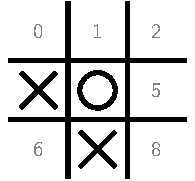
\includegraphics[]{ttt_boards/ttt_69648.pdf}
  \end{minipage}
  \hfill
  \begin{minipage}[t]{0.49\textwidth}
    \centering
    \captionsetup{type=table}
    \captionof{table}{Bewertung Aktionen in Zustand 69648}
    \label{tab:state69648}
    %\begin{table}
%\centering
%\caption{Bewertung Aktionen in Zustand $69648_{10}$}
\begin{tabular}{lrr}
\toprule
Aktion  & Q-Tabelle& W-Tabelle\\ \midrule
0   	& -0,0008	        & 0,0016  \\
1	    & -0,0851	        & -0,1470 \\
2	    & -0,0300       	& -0,1466 \\
5	    & 0,0013	        & -0,1658 \\
6	    & 0,0002        	& 0,0069  \\
8	    & -0,0038	        & 0,0016  \\ \bottomrule
\end{tabular}
%\end{table}
    \end{minipage}
\end{minipage}

Zur Prüfung welche Aktion laut den trainierten \sarsa Agenten die beste erste Aktion für Symbol X ist, wird die durchschnittliche Bewertung von fünf Agenten betrachtet, die in \cref{tab:state0_eval_sarsa} gelistet sind. 
Alle Aktionen, mit Ausnahme der Aktion 4, haben ein negatives Vorzeichen.
Wie die obige Auswertung der Spielstärke der \wtable Agenten zeigt, behindert dies jedoch nicht die Spielstärke des Agenten, da bei der Aktionsauswahl lediglich die Aktion mit dem höchsten \qValue gewählt wird. 
In \cref{tab:state0_eval_sarsa_aggregated} wird die durchschnittliche Bewertung je äquivalenter Aktion betrachtet.
Laut den trainierten Sarsa Agenten ist die Rangfolge der Aktionen: Mitte, Ecke und Kante. 

\begin{table}[!htb]
    \begin{minipage}[t]{.49\textwidth}
        \centering
        \label{tab:state0_eval_sarsa}
        \caption{Bewertung Zustand 0 \\ bester Sarsa Agent}
        \begin{tabular}{lr}
        \toprule
        Aktion  & Bewertung \\ \midrule
        0	& -0,0283 \\
        1	& -0,0258 \\
        2	& -0,0223 \\
        3	& -0,0272 \\
        4	& 0,0019  \\
        5	& -0,0218 \\
        6	& -0,0337 \\
        7	& -0,0394 \\
        8	& -0,0274 \\ \bottomrule
        
        \end{tabular}
    \end{minipage}%
    \begin{minipage}[t]{.49\textwidth}
        \centering
        \caption{Bewertung Aktionsklassen Zustand 0 bester Sarsa Agent}
        \label{tab:state0_eval_sarsa_aggregated}
        \begin{tabular}{lr}
        \toprule
        Aktion  & Bewertung \\ \midrule
        Ecke	& -0,0279 \\
        Kante	& -0,0286 \\
        Mitte	&  0,0019 \\ \bottomrule
        
        \end{tabular}
    \end{minipage}
\end{table}
\section{Vergleich der \qlearning und \sarsa Agenten}

Die trainierten Agenten beider Algorithmen konnten erfolgreich \acl{TTT} durch \splay lernen und Spielstärken erreichen, die über dem implementierten Minimax-Algorithmus liegen. 
\cref{tab:playingAbility_compareAlgorithms_normal} vergleicht die Spielstärke von \bothAlgs, die mit klassischem \splay trainiert wurden. 
Für jede untersuchte Lernrate war die Spielstärke der \qlearning Agenten größer als die von \sarsa. 
\cref{tab:playingAbility_compareAlgorithms_alternate} vergleicht die Spielstärke, die bei alternierendem \splay erreicht werden kann. 
Im Gegensatz zum klassischen \splay erreichen die \sarsa Agenten eine höhere Spielstärke. 
Die \qlearning Agenten verschlechtern sich deutlich bei alternierendem \splay und sind schlechter als der Minimax-Algorithmus. 
Für beide Algorithmen werden mit dem klassischen \splay bessere Ergebnisse erzielt. 
Der jeweils stärkste Agent konnte für $\alpha=0,1$ mit klassischem \splay erzeugt werden. 
Für \qlearning beträgt die durchschnittliche Spielstärke 8.002,72 und für \sarsa 7.905,72. 
Für 150.000 Trainingsepisoden weist \sarsa noch eine leichte Schwäche vor und verliert als Symbol O knapp 1\% seiner Spiele.


Die Verwendung von Afterstates in Form der \wtable verbesserte bei beiden Agenten die Konvergenz.
\cref{fig:convergence_compare_algorithm} vergleicht den Verlauf der Rate optimaler Aktionen während dem Training. Für Symbol X und Symbol O konvergiert der \qlearning Agent schneller und erreicht eine höhere Rate. 
Zudem verbesserte sich die durchschnittliche Spielstärke beider Agenten, wie \cref{tab:playingAbility_compareAlgorithms_experience} zeigt. 
Der \qlearning Agent verbesserte seine Spielstärke um 33,96 auf 8.036,68. 
Die Schwäche von \sarsa wird behoben, sodass dieser als Symbol O keine Spiele mehr verliert.
Die Spielstärke verbessert sich dadurch um 21,96 auf 7.927,68.
Wie jedoch in den jeweiligen Abschnitten angemerkt, ist diese Verbesserung in Relation zur Standardabweichung klein und es liegt nur eine Stichprobenanzahl von $N=5$ vor.

\begin{table}
\centering
\caption[Spielstärke beider Algorithmen unterschiedliche Lernraten, klassisches \splay]{Spielst"arke beider Algorithmen für unterschiedliche Lernraten nach Training mit klassischem \splay}
\label{tab:playingAbility_compareAlgorithms_normal}

\begin{tabular}{lrrr}
\toprule
Lernrate $\alpha$               & Spielst"arke Q-Learning           & Spielst"arke Sarsa                & Differenz QL - Sarsa \\ \midrule
Konstant 0,1                    & 8.002,72 $\pm$ \phantom{0}30,03   & 7.905,72 $\pm$ \phantom{0}75,69   & 97,00 \\
Konstant 0,2                    & 7.801,36 $\pm$ 131,22             & 7.787,94 $\pm$ 105,20             & 13,42 \\
Abnehmend 1 $\rightarrow$ 0,1   & 7.894,92 $\pm$ 132,52             & 7.754,66 $\pm$ 197,59             & 140,26 \\ \bottomrule

\end{tabular}
\end{table}
\begin{table}
\centering
\caption[Spielstärke beider Algorithmen unterschiedliche Lernraten, alternierendes \splay]{Spielst"arke beider Algorithmen für unterschiedliche Lernraten nach Training mit alternierendem \splay}
\label{tab:playingAbility_compareAlgorithms_alternate}

\begin{tabular}{lrrr}
\toprule
Lernrate $\alpha$               & Spielst"arke Q-Learning           & Spielst"arke Sarsa                & Differenz QL - Sarsa \\ \midrule
Konstant 0,1                    & 6.465,66 $\pm$ 481,99             & 6.495,50 $\pm$ 826,74             & \textcolor{red}{-29,84} \\
Konstant 0,2                    & 6.904,92 $\pm$ 399,15             & 7.018,94 $\pm$ 299,04             & \textcolor{red}{-114,02} \\
Abnehmend 1 $\rightarrow$ 0,1   & 6.110,56 $\pm$ 224,66             & 7.625,94 $\pm$ \phantom{0}65,10   & \textcolor{red}{-1.515,38} \\ \bottomrule
\end{tabular}
\end{table}
\begin{table}
\centering
\caption[Spielstärke beider Algorithmen mit \qtable und \wtable, klassisches \splay]{Spielstärke beider Algorithmen mit \qtable und \wtable, klassisches \splay}
\label{tab:playingAbility_compareAlgorithms_experience}

\begin{tabular}{lrrr}
\toprule
Algorithmus                & Spielst"arke Q-Tabelle     & Spielst"arke W-Tabelle              & Q-Tabelle - W-Tabelle \\ \midrule
Q-Learning $\alpha=0,1$    & 8.002,72 $\pm$ 75,69      & 8.036,68 $\pm$ \phantom{0}9,13    & 33,96 \\
Sarsa $\alpha=0,1$         & 7.905,72 $\pm$ 30,03      & 7.927,68 $\pm$ 43,79               & 21,96 \\ \bottomrule
\end{tabular}
\end{table}

\begin{figure}
\centering
\begin{subfigure}[b]{0.75\textwidth}
    \centering
   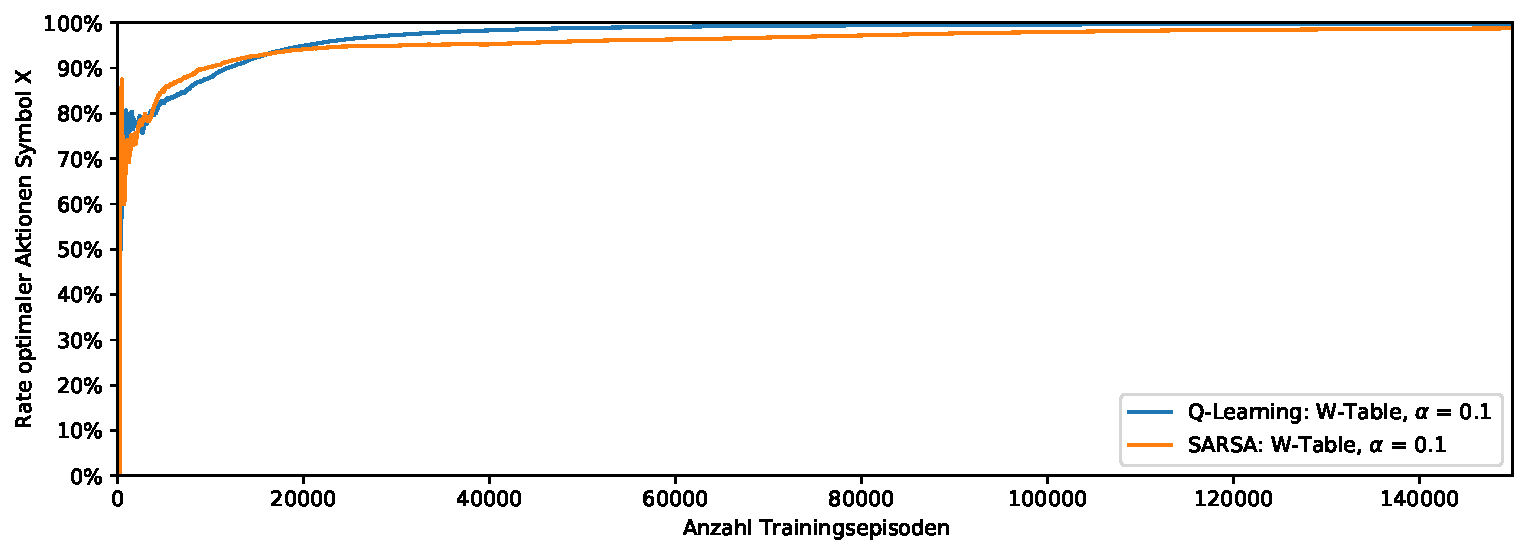
\includegraphics[width=1\linewidth]{convergence/convergence_compare_algorithm_X.pdf}
   \caption{Symbol X}
   \label{fig:convergence_compare_algorithm_X} 
\end{subfigure}

\begin{subfigure}[b]{0.75\textwidth}
    \centering
   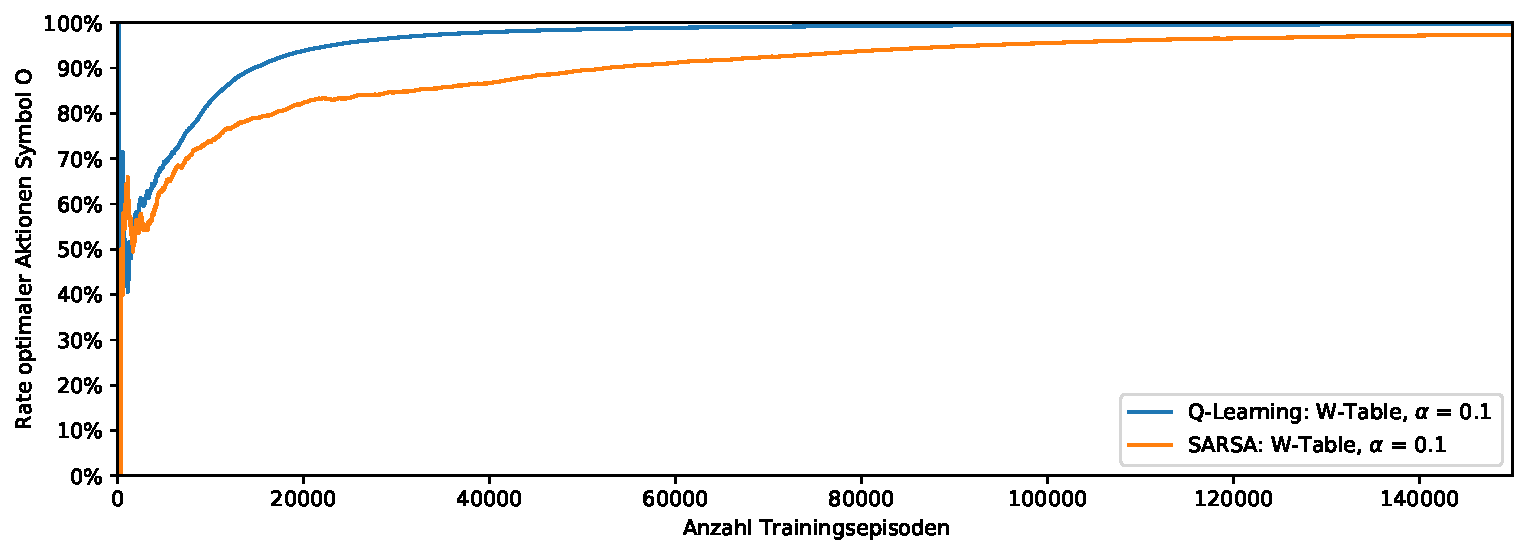
\includegraphics[width=1\linewidth]{convergence/convergence_compare_algorithm_O.pdf}
   \caption{Symbol O}
   \label{fig:convergence_compare_algorithm_O}
\end{subfigure}


\caption[Rate optimaler Aktionen bester \qlearning und \sarsa Agent, \wtable, klassisches \splay]{Rate optimaler Aktionen des besten \qlearning und \sarsa Agenten während dem Training mit \wtable und klassischem \splay (a) Symbol X (b) Symbol O}
\label{fig:convergence_compare_algorithm}
\end{figure}
\section{Beantwortung der Forschungsfragen}
Mit den vorgestellten Ergebnissen können die Forschungsfragen aus \cref{sec:forschungsfragen} wie folgt beantwortet werden:

\textbf{Frage:} Können die Algorithmen Expert Play in \acl{TTT} durch \splay erlernen? \\ \textbf{Antwort:} Die mit den Algorithmen trainierten Agenten spielen besser als der implementierte Minimax-Algorithmus. In den betrachteten Zuständen, zeigten die Agenten Entscheidungen, die mit dem Expert Play konsistent sind. Zur abschließenden Beantwortung ist eine Implementierung der Regeln des Expert Play notwendig, um die Aktionswahl der Agenten zu evaluieren. Die Art des \splay ist entscheidend auf den Trainingserfolg, da beide Agenten mit alternierendem \splay schlechtere Ergebnisse erzielten. Dabei litt Q-Learning unter \splay deutlich mehr als \sarsa. Die erreichte Spielstärke des Q-Learning Agenten ist konsistent mit Experimenten in \cite{mirnovi.QLearningTicTacToe2020}.

\textbf{Frage:} Eine Abschätzung für die Anzahl der Trainingsepisoden, die  ungefähr benötigt werden, um Expert Play in \ac{TTT} durch Self-play zu erlernen? \\ \textbf{Antwort:} In den Vorexperimenten wurde festgestellt, dass mehr als 100.000 Trainingsepisoden notwendig sind, um stabile Ergebnisse zu erhalten. Für die Experimente wurden 150.000 Episoden verwendet, in denen die Agenten Expert Play erlernt haben. Die Auswertung der Konvergenz zeigt zudem, dass Symbol X deutlich schneller konvergiert als Symbol O.

\textbf{Frage:} Welche Auswirkung hat die Verwendung des Konzepts der Afterstates auf das Konvergenzverhalten und Spielstärke der Agenten? \\ \textbf{Antwort:} Durch die Verwendung von Afterstates in Form einer \wtable konnte die Konvergenz und Spielstärke verbessert werden. Die Verbesserungen sind jedoch in Relation zur Standardabweichung gering. Da nur eine Stichprobe von $N=5$ vorliegt, kann nicht abschließend gesagt werden, ob die leichte Verbesserung auf die Nutzung von Afterstates oder Zufall zurückzuführen ist. 

\textbf{Frage:} Was sind die besten Hyperparameter für \bothAlgs? \\ \textbf{Antwort:} Aus der Menge der untersuchten Hyperparameter, erreichten \bothAlgs die besten Ergebnisse, durch folgende Kombination von Hyperparametern:
\begin{itemize}
    \item konstante Lernrate $\alpha=0,1$, 
    \item abnehmende Explorationswahrscheinlichkeit $\epsilon = 1 \rightarrow 0,1$ die nach 2/3 der Trainingsepisoden 0,1 erreicht
    \item Verwendung von Afterstates in Form einer \wtable
\end{itemize}

\textbf{Frage:} Wie unterscheiden sich \bothAlgs hinsichtlich ihrer Konvergenz? \\ \textbf{Antwort:} Q-Learning konvergiert schneller als \sarsa und erreicht eine höhere Rate optimaler Aktionen.

\textbf{Frage:} Welcher Agent erreicht eine bessere Spielstärke, wenn beide RL Agenten mit ihren optimalen Hyperparametern trainiert werden? \\ \textbf{Antwort:} Q-Learning erreicht eine bessere Spielstärke. Wird die Rewardfunktion aus \cref{sec:TDL_TTT} verwendet, lässt sich die Spielstärke quantifizieren. Für Q-Learning beträgt diese im Durchschnitt 8036,68 und für \sarsa 7927,68. Dabei scheint Q-Learning nahezu die maximal mögliche optimale Spielstärke zu erreichen, die auch in mindestens einem anderen Experiment \cite{mirnovi.QLearningTicTacToe2020} gezeigt wurde.

\textbf{Frage:} Was ist aus Sicht der Agenten die optimale erste Aktion? \\ \textbf{Antwort:} \bothAlgs bewerten beide die Aktion \gqq{Mitte} als stärkste erste Aktion für X. Die zweitstärkste Aktion ist das Platzieren eines Symbols in einer der Ecken. Jedoch werden äquivalente Aktionen nicht gemeinsam bewertet, sodass die Frage nicht abschließend beantwortet werden kann. Dass die Mitte, die beste Aktion sein soll, ist jedoch konsistent mit Experimenten, die vorher durchgeführt wurden \cite{kutscheraa.BestOpeningMove2018}. 

\chapter{Konklusion}
In den folgenden Abschnitten werden der Inhalt der Bachelorarbeit und die Ergebnisse der Implementierung für \ac{TTT} zusammengefasst.
Anschließend werden diese kritisch betrachtet bevor ein Ausblick für mögliche weitere Arbeiten gegeben wird.

\section{Zusammenfassung}
In dieser Bachelorarbeit wurden \acl{RL} und die zugehörigen Methoden zur Lösung sequenzieller Entscheidungsprobleme erklärt. 
Der Fokus lag auf dem Teilgebiet des Temporal-Difference Learning und den zugehörigen Algorithmen \bothAlgs.
Die Funktionsweise der Algorithmen wurde erklärt und deren Gemeinsamkeiten sowie Unterschiede aufgezeigt. 
Zur weiteren Untersuchung der Algorithmen und deren Hyperparametern wurden beide für das simple Strategiespiel \acl{TTT} in Java implementiert. 
Untersucht wurden verschiedene Ausprägungen der Lernrate $\alpha$, die im Rahmen von Vorexperimenten festgelegt wurden. 
Zudem wurden die Agenten mit zwei verschiedenen Arten von \splay trainiert. 
Zusätzlich wurde das Konzept der Afterstates in Form einer \wtable implementiert. 
Eine mögliche Definition einer Rewardfunktion wurde erläutert und zum Training der Agenten sowie der Quantifizierung der Spielstärke verwendet. 
Zur Auswertung der trainierten Agenten wurde deren Konvergenz während des Trainings sowie deren Spielstärke gegen einen Minimax-Algorithmus und Spieler mit Zufallstrategie erfasst und verglichen. 
Beide Algorithmen erreichten mit der gleichen Hyperparameterkombination und Nutzung von Afterstates die jeweils besten Agenten, die eine höhere Spielstärke besitzen als der Minimax-Algorithmus. 
Die Auswertung ergab, dass \qlearning im Durchschnitt schneller konvergiert und eine höhere Spielstärke erreicht als \sarsa. 
Verwendet \sarsa keine Afterstates konnten leichte Schwächen für das Symbol O festgestellt werden. 
Beide Agenten bewerteten die \gqq{Mitte} als beste erste Aktion, was konsistent zu anderen Experimenten ist.

\section{Kritische Betrachtung der Inhalte}
In der Arbeit wird ein klassischer Minimax-Algorithmus verwendet. 
Zum einen dient die berechnete Spielstärke des Minimax-Algorithmus als Vergleichsmaßstab bei der Bewertung der Agenten. 
Zum anderen basiert die Konvergenzmetrik auf den Aktionen, die laut des Minimax-Algorithmus optimal sind. 
Wie in \cref{sec:anwendbare_algorithmen} erwähnt, wählt der Agent nicht immer die optimale Aktion, da der Minimax-Algorithmus von einem optimalen Gegner ausgeht. 
Dadurch ist dessen Gewinnrate kleiner, als die optimal mögliche, weil nicht zwischen Aktionen unterschieden wird, die mehr Gewinnchancen haben als andere, wenn das Ergebnis gegen einen optimalen Gegner gleich ist. 
Für die Bewertung der Spielstärke und richtige Rate optimaler Aktionen gemäß \splay sollte daher ein angepasster Minimax-Algorithmus genutzt werden.

Ein weiterer Aspekt ist die Verbesserung des jeweils optimalen Agenten durch das Konzept der Afterstates in Form der \wtable. Relativ zur Spielstärke ist die erzielte Verbesserung klein, sodass nicht gesagt werden kann, ob diese Verbesserung nur durch Zufall entstanden ist oder wirklich auf den \wtable zurückgeführt werden kann. Da wegen der Zeitbeschränkung nur fünf Agenten trainiert wurden, ist die Stichprobe zu gering für einen Signifikanztest. Um den Wert zu stabilisieren, sollten daher mehr Agenten trainiert werden.

Eine weitere Limitierung besteht in der Menge der getesteten Hyperparameterkombinationen und Methoden, wie diese während des Trainings reduziert werden können. Durch Vorexperimente wurde versucht diese möglichst sinnvoll zu wählen, aber es kann nicht ausgeschlossen werden, dass mit anderen Werten stärkere Ergebnisse möglich sind.

\section{Anmerkungen f"ur k"unftige Arbeiten}
Wie im obigen Abschnitt angemerkt, liegt eine mögliche Verbesserung in der Evaluation durch den Minimax-Algorithmus.
Um dies zu erreichen könnte ein Spieler implementiert werden, der die im Expert Play formulierten Regeln genau befolgt. 
Eine weitere Möglichkeit ist die Erweiterung des bestehenden Minimax-Algorithmus, sodass zur Bewertung der Aktionen neben dem zu erwartenden Reward auch die Anzahl potenzieller Gewinnmöglichkeiten genutzt wird.
Haben zwei Aktionen einen gleich hohen Reward, wird die Aktion als optimal deklariert, die mehr Gewinnmöglichkeiten für den Agenten bietet.
Neben der Verbesserung der Evaluation, könnte es lohnend sein die implementierten Standardversionen der Algorithmen mit abgewandelten Formen wie Double \qlearning, Expected \sarsa \cite[S. 133ff.]{suttonReinforcementLearningIntroduction2018}, \cite{littmanMarkovGamesFramework1994} oder neuronalen Netzen \cite{konenParameterSelection2008} zu vergleichen  . 
Zudem wäre ein Vergleich mit Algorithmen interessant, die im Gegensatz zu den implementierten Algorithmen für Multi-Agenten \ac{RL} vorgesehen sind. 
Insbesondere sogenannte Equilibrium Learners wären gut geeignet, da diese sich auf Nullsummenspiele wie \ac{TTT} fokussieren. \cite[S. 39]{netoSingleAgentMultiAgentReinforcement} 
Außerdem gibt es neben dem Konzept der Afterstates weitere Möglichkeiten, um die Lerndaten effektiver zu nutzen wie z.B. Eligibility Traces \cite{singhReinforcementLearningReplacing1996} oder die generelle Reduktion des Zustandsraums durch bessere Enkodierung. 
Letzteres ist im Falle von \ac {TTT} besonders interessant, da es für jeden Zustand bis zu acht weitere äquivalente Zustände geben kann.

\vspace{1cm}
\textbf{Wörterzählung}: 12.614 Worte


\pagenumbering{Roman}

\setcounter{page}{\value{romanConsecutive}}
\printbibliography[title={Literaturverzeichnis}]
\appendix
\clearpage
\pdfbookmark{Anhang}{anhang}

\addcontentsline{toc}{chapter}{Anhang}


\chapter{Model of Expert Performance}
\label{chap:ModelofExpert}

\begin{figure}[h]
    \centering
    \frame{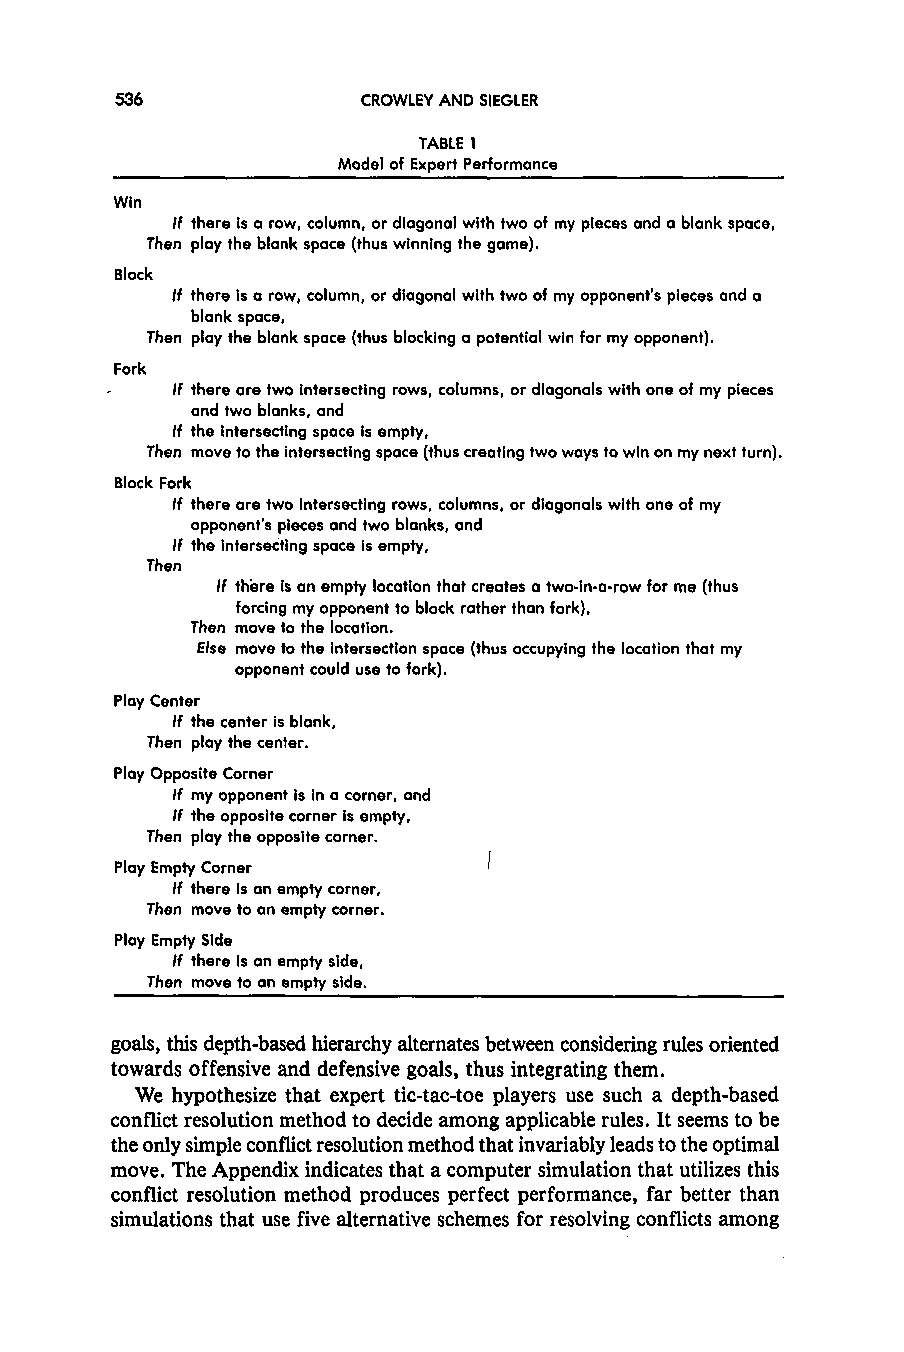
\includegraphics[width=0.7\linewidth]{04_Artefakte/crowley_expertplay.pdf}}
    \caption[Model of Expert Performance]{Model of Expert Performance von \citeauthor{crowleyFlexibleStrategyUse1993}, Auszug aus \cite[S. 536]{crowleyFlexibleStrategyUse1993}}
\end{figure}

\chapter{Beispiel für Meta-Log der Implementierung}
\label{chap:meta}
\begin{longlisting}
\caption{Meta-Log der Implementierung}
\label{listing:meta}
\inputminted{text}{04_Artefakte/03_Listings/meta.txt}
\end{longlisting}



\chapter{minimax-Methode}
\label{chap:minimax_listing}
\begin{longlisting}
\caption{minimax-Methode der Klasse MinimaxAlgorithm}
\label{listing:minimax}
\inputminted{java}{04_Artefakte/03_Listings/minimax.java}
\end{longlisting}



\chapter{Zusätzliche Auswertung zu Q-Learning}
\label{chap:app_qlearning}
\section{Konvergenz alternierendes Self-play}

\begin{figure}[h]
\centering
\begin{subfigure}[b]{0.75\textwidth}
    \centering
   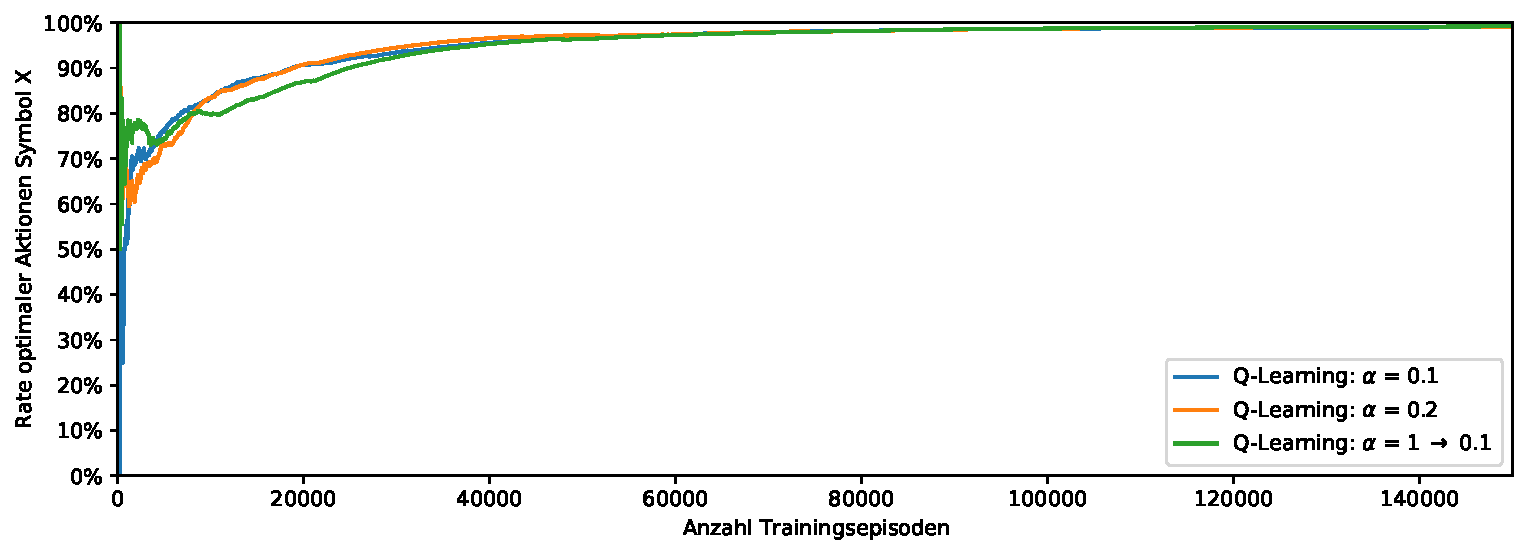
\includegraphics[width=1\linewidth]{convergence/convergence_compare_alpha_QLearning_ALTERNATE_X.pdf}
   \caption{Symbol X}
   \label{fig:convergence_compare_alpha_QLearning_ALTERNATE_X} 
\end{subfigure}

\begin{subfigure}[b]{0.75\textwidth}
    \centering
   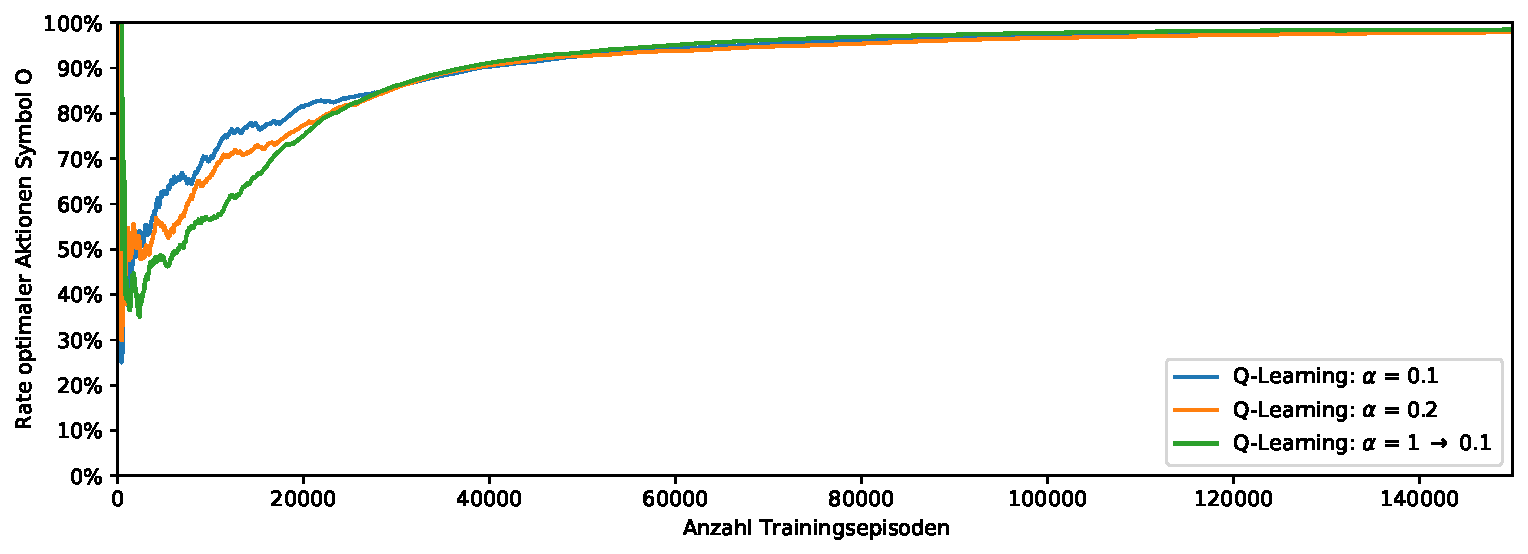
\includegraphics[width=1\linewidth]{convergence/convergence_compare_alpha_QLearning_ALTERNATE_O.pdf}
   \caption{Sybmol O}
   \label{fig:convergence_compare_alpha_QLearning_ALTERNATE_O}
\end{subfigure}
\caption[Rate optimaler Aktionen Q-Learning unterschiedliche Lernraten, alternierendes \splay]{Rate optimaler Aktionen von Q-Learning für verschiedene Lernraten $\alpha$, alternierendes \splay (a) Symbol X (b) Symbol O}
\label{fig:convergence_compare_alpha_QLearning_ALTERNATE}
\end{figure}

\section{Spielergebnismatritzen klassisches Self-play}
\begin{table}[ht]
\centering
\caption[Spielergebnismatrix \qlearning: $\alpha=0,2$, klassisches \splay]{Spielergebnismatrix für \qlearning mit Lernrate $\alpha=0,2$, klassisches \splay}
\label{tab:resultmatrix_ql_normal_alpha02}

\begin{tabular}{llrlr}
\toprule
 & \multicolumn{2}{l}{\textbf{Minimax}} & \multicolumn{2}{l}{\textbf{Random}} \\ \midrule
\textbf{X Q-Learning}   & X Q-Learning:     & 0,00\% $\pm$    0,00\%            & X Q-Learning:         & 98,91\% $\pm$ 0,31\%  \\
                        & O Minimax:        & 0,00\% $\pm$    0,00\%            & O Random:             & 0,00\% $\pm$  0,00\%  \\
                        & Unentschieden:    & 100,00\% $\pm$  0,00\%            & Unentschieden:        & 1,09\% $\pm$  0,31\%  \\ \cmidrule{2-5}
\textbf{O Q-Learning}   & X Minimax:        & 0,00\% $\pm$    0,00\%            & X Random:             & 0,00\% $\pm$  0,00\%  \\
                        & O Q-Learning:     & 0,00\% $\pm$    0,00\%            & O Q-Learning:         & 90,84\% $\pm$ 0,49\%  \\
                        & Unentschieden:    & 100,00\% $\pm$  0,00\%            & Unentschieden:        & 9,16\% $\pm$  0,49\%  \\ \bottomrule
\end{tabular}
\end{table}
\begin{table}[h]
\centering
\caption[Spielergebnismatrix \qlearning: abnehmende Lernrate, klassisches \splay]{Spielergebnismatrix für \qlearning mit abnehmender Lernrate, klassisches \splay}
\label{tab:resultmatrix_ql_normal_alpha_decay}

\begin{tabular}{llrlr}
\toprule
 & \multicolumn{2}{l}{\textbf{Minimax}} & \multicolumn{2}{l}{\textbf{Random}} \\ \midrule
\textbf{X Q-Learning}   & X Q-Learning:     & 0,00\% $\pm$    0,00\%            & X Q-Learning:         & 98,91\% $\pm$ 0,24\%  \\
                        & O Minimax:        & 0,00\% $\pm$    0,00\%            & O Random:             & 0,00\% $\pm$  0,00\%  \\
                        & Unentschieden:    & 100,00\% $\pm$  0,00\%            & Unentschieden:        & 1,09\% $\pm$  0,24\%  \\ \cmidrule{2-5}
\textbf{O Q-Learning}   & X Minimax:        & 0,00\% $\pm$    0,00\%            & X Random:             & 0,00\% $\pm$  0,00\%  \\
                        & O Q-Learning:     & 0,00\% $\pm$    0,00\%            & O Q-Learning:         & 91,49\% $\pm$ 0,35\%  \\
                        & Unentschieden:    & 100,00\% $\pm$  0,00\%            & Unentschieden:        & 8,51\% $\pm$  0,35\%  \\ \bottomrule
\end{tabular}
\end{table}

\section{Spielergebnismatritzen alternierendes Self-play}

\begin{table}[ht]
\centering
\caption[Spielergebnismatrix \qlearning: $\alpha=0,1$, alternierendes \splay]{Spielergebnismatrix für \qlearning mit Lernrate $\alpha=0,1$, alternierendes \splay}
\label{tab:resultmatrix_ql_alternate_alpha01}

\begin{tabular}{llrlr}
\toprule
 & \multicolumn{2}{l}{\textbf{Minimax}} & \multicolumn{2}{l}{\textbf{Random}} \\ \midrule
\textbf{X Q-Learning}   & X Q-Learning:     & 0,00\% $\pm$    0,00\%            & X Q-Learning:         & 95,12\% $\pm$ 1,75\%  \\
                        & O Minimax:        & 0,00\% $\pm$    0,00\%            & O Random:             & 0,22\% $\pm$  0,16\%  \\
                        & Unentschieden:    & 100,00\% $\pm$  0,00\%            & Unentschieden:        & 4,66\% $\pm$  1,64\%  \\ \cmidrule{2-5}
\textbf{O Q-Learning}   & X Minimax:        & 0,00\% $\pm$    0,00\%            & X Random:             & 0,96\% $\pm$  0,50\%  \\
                        & O Q-Learning:     & 0,00\% $\pm$    0,00\%            & O Q-Learning:         & 81,96\% $\pm$ 2,49\%  \\
                        & Unentschieden:    & 100,00\% $\pm$  0,00\%            & Unentschieden:        & 17,08\% $\pm$ 2,59\%  \\ \bottomrule
\end{tabular}
\end{table}
\begin{table}[ht]
\centering
\caption[Spielergebnismatrix \qlearning: $\alpha=0,2$, alternierendes \splay]{Spielergebnismatrix für \qlearning mit Lernrate $\alpha=0,2$, alternierendes \splay}
\label{tab:resultmatrix_ql_alternate_alpha02}

\begin{tabular}{llrlr}
\toprule
 & \multicolumn{2}{l}{\textbf{Minimax}} & \multicolumn{2}{l}{\textbf{Random}} \\ \midrule
\textbf{X Q-Learning}   & X Q-Learning:     & 0,00\% $\pm$    0,00\%            & X Q-Learning:         & 96,52\% $\pm$ 2,72\%  \\
                        & O Minimax:        & 0,00\% $\pm$    0,00\%            & O Random:             & 0,07\% $\pm$  0,09\%  \\
                        & Unentschieden:    & 100,00\% $\pm$  0,00\%            & Unentschieden:        & 3,41\% $\pm$  2,63\%  \\ \cmidrule{2-5}
\textbf{O Q-Learning}   & X Minimax:        & 0,04\% $\pm$    0,09\%            & X Random:             & 0,47\% $\pm$  0,18\%  \\
                        & O Q-Learning:     & 0,00\% $\pm$    0,00\%            & O Q-Learning:         & 84,37\% $\pm$ 1,94\%  \\
                        & Unentschieden:    & 99,96\% $\pm$   0,09\%            & Unentschieden:        & 15,17\% $\pm$ 1,93\%  \\ \bottomrule
\end{tabular}
\end{table}
\begin{table}[htbp]
\centering
    \caption[Spielergebnismatrix \qlearning: abnehmende Lernrate, alternierendes \splay]{Spielergebnismatrix für \qlearning mit abnehmender Lernrate, alternierendes \splay}
    \label{tab:resultmatrix_ql_alternate_alpha_decay}
    \begin{tabular}{llrlr}
    \toprule
     & \multicolumn{2}{l}{\textbf{Minimax}} & \multicolumn{2}{l}{\textbf{Random}} \\ \midrule
    \textbf{X Q-Learning}   & X Q-Learning:     & 0,00\% $\pm$    0,00\%            & X Q-Learning:         & 93,85\% $\pm$  0,57\%  \\
                            & O Minimax:        & 0,00\% $\pm$    0,00\%            & O Random:             & 0,21\% $\pm$   0,11\%  \\
                            & Unentschieden:    & 100,00\% $\pm$  0,00\%            & Unentschieden:        & 5,94\% $\pm$   0,47\%  \\ \cmidrule{2-5}
    \textbf{O Q-Learning}   & X Minimax:        & 0,40\% $\pm$    0,80\%            & X Random:             & 0,28\% $\pm$   0,37\%  \\
                            & O Q-Learning:     & 0,00\% $\pm$    0,00\%            & O Q-Learning:         & 79,32\% $\pm$  3,14\%  \\
                            & Unentschieden:    & 99,60\% $\pm$   0,80\%            & Unentschieden:        & 20,40\% $\pm$  2,96\%  \\ \bottomrule
    \end{tabular}
\end{table}


\chapter{Zusätzliche Auswertung zu Sarsa}
\label{chap:app_sarsa}
\section{Konvergenz alternierendes Self-play}

\begin{figure}[h]
\centering
\begin{subfigure}[b]{0.75\textwidth}
    \centering
   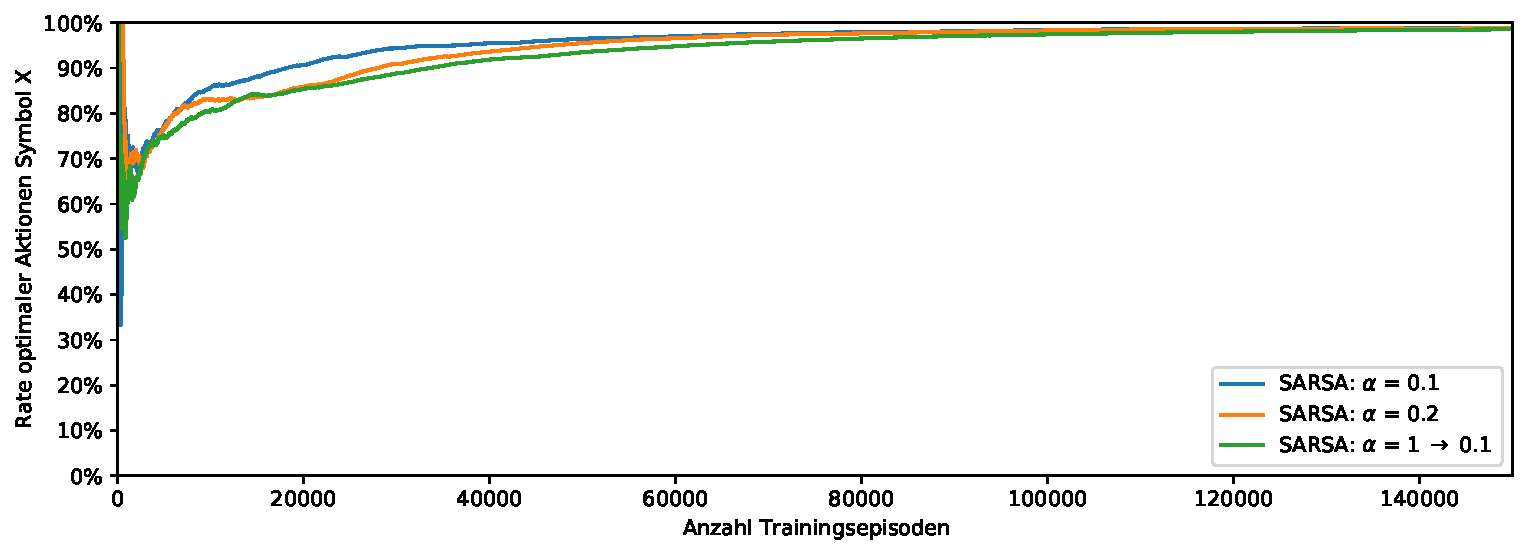
\includegraphics[width=1\linewidth]{convergence/convergence_compare_alpha_SARSA_ALTERNATE_X.pdf}
   \caption{Symbol X}
   \label{fig:convergence_compare_alpha_SARSA_ALTERNATE_X} 
\end{subfigure}

\begin{subfigure}[b]{0.75\textwidth}
    \centering
   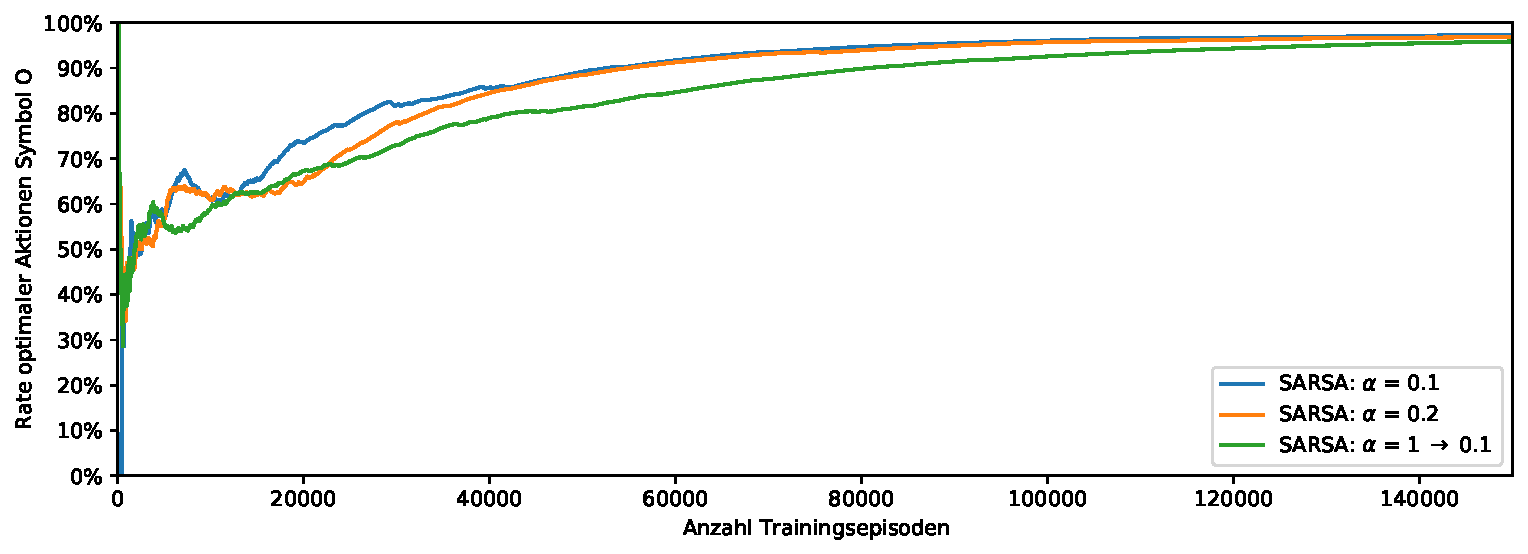
\includegraphics[width=1\linewidth]{convergence/convergence_compare_alpha_SARSA_ALTERNATE_O.pdf}
   \caption{Sybmol O}
   \label{fig:convergence_compare_alpha_SARSA_ALTERNATE_O}
\end{subfigure}

\caption[Rate optimaler Aktionen \sarsa unterschiedliche Lernraten, alternierendes \splay]{Rate optimaler Aktionen von \sarsa für verschiedene Lernraten $\alpha$, alternierendes \splay (a) Symbol X (b) Symbol O}
\label{fig:convergence_compare_alpha_SARSA_ALTERNATE}
\end{figure}

\section{Spielergebnismatritzen klassisches Self-play}
\begin{table}
\centering
\caption[Spielergebnismatrix \sarsa: $\alpha=0,2$, klassisches \splay]{Spielergebnismatrix für \sarsa mit Lernrate $\alpha=0,2$, klassisches \splay}
%\label{tab:resultmatrix_sarsa_normal_alpha02}

\begin{tabular}{llrlr}
\toprule
 & \multicolumn{2}{l}{\textbf{Minimax}} & \multicolumn{2}{l}{\textbf{Random}} \\ \midrule
\textbf{X Sarsa}        & X Sarsa:          & 0,00\% $\pm$    0,00\%            & X Sarsa:              & 98,92\% $\pm$ 0,09\%  \\
                        & O Minimax:        & 0,00\% $\pm$    0,00\%            & O Random:             & 0,00\% $\pm$  0,00\%  \\
                        & Unentschieden:    & 100,00\% $\pm$  0,00\%            & Unentschieden:        & 1,08\% $\pm$  0,09\%  \\ \cmidrule{2-5}
\textbf{O Sarsa}        & X Minimax:        & 0,85\% $\pm$    1,05\%            & X Random:             & 0,18\% $\pm$  0,16\%  \\
                        & O Sarsa:          & 0,00\% $\pm$    0,00\%            & O Sarsa:              & 87,25\% $\pm$ 1,37\%  \\
                        & Unentschieden:    & 99,15\% $\pm$   1,05\%            & Unentschieden:        & 12,57\% $\pm$ 1,21\%  \\ \bottomrule
\end{tabular}
\end{table}
\begin{table}
\centering
\caption[Spielergebnismatrix \sarsa: abnehmende Lernrate, klassisches \splay]{Spielergebnismatrix für \sarsa mit abnehmender Lernrate, klassisches \splay}
%\label{tab:resultmatrix_sarsa_normal_alpha_decay}

\begin{tabular}{llrlr}
\toprule
 & \multicolumn{2}{l}{\textbf{Minimax}} & \multicolumn{2}{l}{\textbf{Random}} \\ \midrule
\textbf{X Sarsa}        & X Sarsa:          & 0,00\% $\pm$    0,00\%            & X Sarsa:              & 98,68\% $\pm$ 0,50\%  \\
                        & O Minimax:        & 0,00\% $\pm$    0,00\%            & O Random:             & 0,00\% $\pm$  0,00\%  \\
                        & Unentschieden:    & 100,00\% $\pm$  0,00\%            & Unentschieden:        & 1,32\% $\pm$  0,50\%  \\ \cmidrule{2-5}
\textbf{O Sarsa}        & X Minimax:        & 0,73\% $\pm$    1,18\%            & X Random:             & 0,14\% $\pm$ 0,18\%  \\
                        & O Sarsa:          & 0,00\% $\pm$    0,00\%            & O Sarsa:              & 87,19\% $\pm$ 2,22\%  \\
                        & Unentschieden:    & 99,27\% $\pm$   1,18\%            & Unentschieden:        & 12,67\% $\pm$ 2,12\%  \\ \bottomrule
\end{tabular}
\end{table}

\section{Spielergebnismatritzen alternierendes Self-play}

\begin{table}[!h]
\centering
\caption[Spielergebnismatrix \sarsa: $\alpha=0,1$, alternierendes \splay]{Spielergebnismatrix für \sarsa mit Lernrate $\alpha=0,1$, alternierendes \splay}
%\label{tab:resultmatrix_sarsa_alternate_alpha01}

\begin{tabular}{llrlr}
\toprule
 & \multicolumn{2}{l}{\textbf{Minimax}} & \multicolumn{2}{l}{\textbf{Random}} \\ \midrule
\textbf{X Sarsa}        & X Sarsa:          & 0,00\% $\pm$    0,00\%            & X Sarsa:              & 95,97\% $\pm$ 2,93\%  \\
                        & O Minimax:        & 8,81\% $\pm$    15,25\%           & O Random:             & 1,38\% $\pm$  2,02\%  \\
                        & Unentschieden:    & 91,19\% $\pm$   15,25\%           & Unentschieden:        & 2,65\% $\pm$  1,03\%  \\ \cmidrule{2-5}
\textbf{O Sarsa}        & X Minimax:        & 3,29\% $\pm$    4,41\%            & X Random:             & 2,48\% $\pm$  0,51\%  \\
                        & O Sarsa:          & 0,00\% $\pm$    0,00\%            & O Sarsa:              & 84,36\% $\pm$ 1,09\%  \\
                        & Unentschieden:    & 96,71\% $\pm$   4,41\%            & Unentschieden:        & 13,15\% $\pm$ 0,96\%  \\ \bottomrule
\end{tabular}
\end{table}
\begin{table}[!h]
\centering
\caption[Spielergebnismatrix \sarsa: $\alpha=0,2$, alternierendes \splay]{Spielergebnismatrix für \sarsa mit Lernrate $\alpha=0,2$, alternierendes \splay}
%\label{tab:resultmatrix_sarsa_alternate_alpha02}

\begin{tabular}{llrlr}
\toprule
 & \multicolumn{2}{l}{\textbf{Minimax}} & \multicolumn{2}{l}{\textbf{Random}} \\ \midrule
\textbf{X Sarsa}        & X Sarsa:          & 0,00\% $\pm$    0,00\%            & X Sarsa:              & 97,15\% $\pm$ 1,42\%  \\
                        & O Minimax:        & 0,00\% $\pm$    0,00\%            & O Random:             & 0,60\% $\pm$  0,63\%  \\
                        & Unentschieden:    & 100,00\% $\pm$  0,00\%            & Unentschieden:        & 2,25\% $\pm$  0,84\%  \\ \cmidrule{2-5}
\textbf{O Sarsa}        & X Minimax:        & 3,29\% $\pm$    4,17\%            & X Random:             & 1,54\% $\pm$  0,62\%  \\
                        & O Sarsa:          & 0,00\% $\pm$    0,00\%            & O Sarsa:              & 85,22\% $\pm$ 1,19\%  \\
                        & Unentschieden:    & 96,71\% $\pm$   4,17\%            & Unentschieden:        & 13,24\% $\pm$ 1,19\%  \\ \bottomrule
\end{tabular}
\end{table}
\begin{table}[!t]
\centering
\caption[Spielergebnismatrix \sarsa: abnehmende Lernrate, alternierendes \splay]{Spielergebnismatrix für \sarsa mit abnehmender Lernrate, alternierendes \splay}
%\label{tab:resultmatrix_sarsa_alternate_alpha_decay}

\begin{tabular}{llrlr}
\toprule
 & \multicolumn{2}{l}{\textbf{Minimax}} & \multicolumn{2}{l}{\textbf{Random}} \\ \midrule
\textbf{X Sarsa}        & X Sarsa:          & 0,00\% $\pm$    0,00\%            & X Sarsa:              & 98,80\% $\pm$ 0,10\%  \\
                        & O Minimax:        & 0,00\% $\pm$    0,00\%            & O Random:             & 0,00\% $\pm$  0,00\%  \\
                        & Unentschieden:    & 100,00\% $\pm$  0,00\%            & Unentschieden:        & 1,20\% $\pm$  0,10\%  \\ \cmidrule{2-5}
\textbf{O Sarsa}        & X Minimax:        & 0,00\% $\pm$    0,00\%            & X Random:             & 0,38\% $\pm$  0,20\%  \\
                        & O Sarsa:          & 0,00\% $\pm$    0,00\%            & O Sarsa:              & 86,83\% $\pm$ 0,54\%  \\
                        & Unentschieden:    & 100,00\% $\pm$  0,00\%            & Unentschieden:        & 12,79\% $\pm$ 0,37\%  \\ \bottomrule
\end{tabular}
\end{table}

\usestandardtocs
\bookmarksetup{startatroot}% siehe bookmark-Anleitung

\end{document}
